\documentclass[twoside]{book}

% Packages required by doxygen
\usepackage{calc}
\usepackage{doxygen}
\usepackage{graphicx}
\usepackage[utf8]{inputenc}
\usepackage{makeidx}
\usepackage{multicol}
\usepackage{multirow}
\usepackage{textcomp}
\usepackage[table]{xcolor}

% Font selection
\usepackage[T1]{fontenc}
\usepackage{mathptmx}
\usepackage[scaled=.90]{helvet}
\usepackage{courier}
\usepackage{amssymb}
\usepackage{sectsty}
\renewcommand{\familydefault}{\sfdefault}
\allsectionsfont{%
  \fontseries{bc}\selectfont%
  \color{darkgray}%
}
\renewcommand{\DoxyLabelFont}{%
  \fontseries{bc}\selectfont%
  \color{darkgray}%
}

% Page & text layout
\usepackage{geometry}
\geometry{%
  a4paper,%
  top=2.5cm,%
  bottom=2.5cm,%
  left=2.5cm,%
  right=2.5cm%
}
\tolerance=750
\hfuzz=15pt
\hbadness=750
\setlength{\emergencystretch}{15pt}
\setlength{\parindent}{0cm}
\setlength{\parskip}{0.2cm}
\makeatletter
\renewcommand{\paragraph}{%
  \@startsection{paragraph}{4}{0ex}{-1.0ex}{1.0ex}{%
    \normalfont\normalsize\bfseries\SS@parafont%
  }%
}
\renewcommand{\subparagraph}{%
  \@startsection{subparagraph}{5}{0ex}{-1.0ex}{1.0ex}{%
    \normalfont\normalsize\bfseries\SS@subparafont%
  }%
}
\makeatother

% Headers & footers
\usepackage{fancyhdr}
\pagestyle{fancyplain}
\fancyhead[LE]{\fancyplain{}{\bfseries\thepage}}
\fancyhead[CE]{\fancyplain{}{}}
\fancyhead[RE]{\fancyplain{}{\bfseries\leftmark}}
\fancyhead[LO]{\fancyplain{}{\bfseries\rightmark}}
\fancyhead[CO]{\fancyplain{}{}}
\fancyhead[RO]{\fancyplain{}{\bfseries\thepage}}
\fancyfoot[LE]{\fancyplain{}{}}
\fancyfoot[CE]{\fancyplain{}{}}
\fancyfoot[RE]{\fancyplain{}{\bfseries\scriptsize Generated on Sat Nov 11 2017 20\-:52\-:17 for Facial Recognition by Doxygen }}
\fancyfoot[LO]{\fancyplain{}{\bfseries\scriptsize Generated on Sat Nov 11 2017 20\-:52\-:17 for Facial Recognition by Doxygen }}
\fancyfoot[CO]{\fancyplain{}{}}
\fancyfoot[RO]{\fancyplain{}{}}
\renewcommand{\footrulewidth}{0.4pt}
\renewcommand{\chaptermark}[1]{%
  \markboth{#1}{}%
}
\renewcommand{\sectionmark}[1]{%
  \markright{\thesection\ #1}%
}

% Indices & bibliography
\usepackage{natbib}
\usepackage[titles]{tocloft}
\setcounter{tocdepth}{3}
\setcounter{secnumdepth}{5}
\makeindex

% Hyperlinks (required, but should be loaded last)
\usepackage{ifpdf}
\ifpdf
  \usepackage[pdftex,pagebackref=true]{hyperref}
\else
  \usepackage[ps2pdf,pagebackref=true]{hyperref}
\fi
\hypersetup{%
  colorlinks=true,%
  linkcolor=blue,%
  citecolor=blue,%
  unicode%
}

% Custom commands
\newcommand{\clearemptydoublepage}{%
  \newpage{\pagestyle{empty}\cleardoublepage}%
}


%===== C O N T E N T S =====

\begin{document}

% Titlepage & ToC
\hypersetup{pageanchor=false}
\pagenumbering{roman}
\begin{titlepage}
\vspace*{7cm}
\begin{center}%
{\Large Facial Recognition }\\
\vspace*{1cm}
{\large Generated by Doxygen 1.8.6}\\
\vspace*{0.5cm}
{\small Sat Nov 11 2017 20:52:17}\\
\end{center}
\end{titlepage}
\clearemptydoublepage
\tableofcontents
\clearemptydoublepage
\pagenumbering{arabic}
\hypersetup{pageanchor=true}

%--- Begin generated contents ---
\chapter{Class Index}
\section{Class List}
Here are the classes, structs, unions and interfaces with brief descriptions\-:\begin{DoxyCompactList}
\item\contentsline{section}{\hyperlink{struct__matrix}{\-\_\-matrix} \\*Matrix between matrix and vector they are able to be casted into one another }{\pageref{struct__matrix}}{}
\item\contentsline{section}{\hyperlink{struct__vector}{\-\_\-vector} \\*Vector padding is to make sure that matrix and vector both have the same byte size and allignment between matrix and vector they are able to be casted into one another }{\pageref{struct__vector}}{}
\end{DoxyCompactList}

\chapter{File Index}
\section{File List}
Here is a list of all documented files with brief descriptions\-:\begin{DoxyCompactList}
\item\contentsline{section}{/mnt/c/\-A\-B\-C/\-C\-S/github/\-Facial-\/\-Recognition/src/\hyperlink{facerec_8c}{facerec.\-c} \\*File containing the main function }{\pageref{facerec_8c}}{}
\item\contentsline{section}{/mnt/c/\-A\-B\-C/\-C\-S/github/\-Facial-\/\-Recognition/src/libs/\hyperlink{linalg_8c}{linalg.\-c} \\*File containing common linear algebra functions }{\pageref{linalg_8c}}{}
\item\contentsline{section}{/mnt/c/\-A\-B\-C/\-C\-S/github/\-Facial-\/\-Recognition/src/libs/\hyperlink{linalg_8h}{linalg.\-h} \\*File containing common linear algebra functions }{\pageref{linalg_8h}}{}
\item\contentsline{section}{/mnt/c/\-A\-B\-C/\-C\-S/github/\-Facial-\/\-Recognition/src/libs/\hyperlink{tiff__util_8c}{tiff\-\_\-util.\-c} \\*File containing common libtiff wrapper functions }{\pageref{tiff__util_8c}}{}
\item\contentsline{section}{/mnt/c/\-A\-B\-C/\-C\-S/github/\-Facial-\/\-Recognition/src/libs/\hyperlink{tiff__util_8h}{tiff\-\_\-util.\-h} \\*File containing common libtiff wrapper functions }{\pageref{tiff__util_8h}}{}
\end{DoxyCompactList}

\chapter{Class Documentation}
\hypertarget{struct__matrix}{\section{\-\_\-matrix Struct Reference}
\label{struct__matrix}\index{\-\_\-matrix@{\-\_\-matrix}}
}


represents a matrix between matrix and vector they are able to be casted into one another  




{\ttfamily \#include $<$linalg.\-h$>$}



Collaboration diagram for \-\_\-matrix\-:
\nopagebreak
\begin{figure}[H]
\begin{center}
\leavevmode
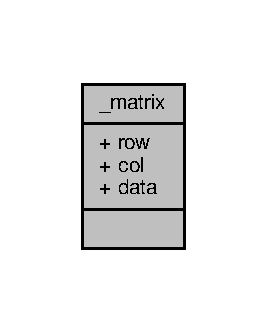
\includegraphics[width=128pt]{struct__matrix__coll__graph}
\end{center}
\end{figure}
\subsection*{Public Attributes}
\begin{DoxyCompactItemize}
\item 
\hypertarget{struct__matrix_a1087bec6a11b0773b4852c4ca49fc32a}{size\-\_\-t \hyperlink{struct__matrix_a1087bec6a11b0773b4852c4ca49fc32a}{row}}\label{struct__matrix_a1087bec6a11b0773b4852c4ca49fc32a}

\begin{DoxyCompactList}\small\item\em the number of rows in the matrix \end{DoxyCompactList}\item 
\hypertarget{struct__matrix_a7e9feb52cfc0a9d7cba5320abcaa997a}{size\-\_\-t \hyperlink{struct__matrix_a7e9feb52cfc0a9d7cba5320abcaa997a}{col}}\label{struct__matrix_a7e9feb52cfc0a9d7cba5320abcaa997a}

\begin{DoxyCompactList}\small\item\em the number of columns in the matrix \end{DoxyCompactList}\item 
\hypertarget{struct__matrix_ab0c92b382e007327a4cc5fc6818c77a9}{double \hyperlink{struct__matrix_ab0c92b382e007327a4cc5fc6818c77a9}{data} \mbox{[}$\,$\mbox{]}}\label{struct__matrix_ab0c92b382e007327a4cc5fc6818c77a9}

\begin{DoxyCompactList}\small\item\em row wise expansion of the elements in the matrix \end{DoxyCompactList}\end{DoxyCompactItemize}


\subsection{Detailed Description}
represents a matrix between matrix and vector they are able to be casted into one another 

The documentation for this struct was generated from the following file\-:\begin{DoxyCompactItemize}
\item 
/mnt/c/\-A\-B\-C/\-C\-S/github/\-Facial-\/\-Recognition/src/libs/\hyperlink{linalg_8h}{linalg.\-h}\end{DoxyCompactItemize}

\hypertarget{struct__vector}{\section{\-\_\-vector Struct Reference}
\label{struct__vector}\index{\-\_\-vector@{\-\_\-vector}}
}


represents a vector padding is to make sure that matrix and vector both have the same byte size and allignment between matrix and vector they are able to be casted into one another  




{\ttfamily \#include $<$linalg.\-h$>$}



Collaboration diagram for \-\_\-vector\-:\nopagebreak
\begin{figure}[H]
\begin{center}
\leavevmode
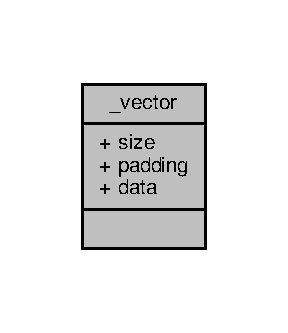
\includegraphics[width=138pt]{struct__vector__coll__graph}
\end{center}
\end{figure}
\subsection*{Public Attributes}
\begin{DoxyCompactItemize}
\item 
\hypertarget{struct__vector_a1ed8dca78f3e589deb8dad9b53aec3fa}{size\-\_\-t \hyperlink{struct__vector_a1ed8dca78f3e589deb8dad9b53aec3fa}{size}}\label{struct__vector_a1ed8dca78f3e589deb8dad9b53aec3fa}

\begin{DoxyCompactList}\small\item\em the number of elements in the vector \end{DoxyCompactList}\item 
\hypertarget{struct__vector_a4165a40cc39bfd874677299c943b290f}{size\-\_\-t \hyperlink{struct__vector_a4165a40cc39bfd874677299c943b290f}{padding}}\label{struct__vector_a4165a40cc39bfd874677299c943b290f}

\begin{DoxyCompactList}\small\item\em unused value but important as padding \end{DoxyCompactList}\item 
\hypertarget{struct__vector_abcf7d1342126a90769b2a05126897859}{double \hyperlink{struct__vector_abcf7d1342126a90769b2a05126897859}{data} \mbox{[}$\,$\mbox{]}}\label{struct__vector_abcf7d1342126a90769b2a05126897859}

\begin{DoxyCompactList}\small\item\em the elements of the vector \end{DoxyCompactList}\end{DoxyCompactItemize}


\subsection{Detailed Description}
represents a vector padding is to make sure that matrix and vector both have the same byte size and allignment between matrix and vector they are able to be casted into one another 

The documentation for this struct was generated from the following file\-:\begin{DoxyCompactItemize}
\item 
/mnt/c/\-A\-B\-C/\-C\-S/github/\-Facial-\/\-Recognition/src/libs/\hyperlink{linalg_8h}{linalg.\-h}\end{DoxyCompactItemize}

\chapter{File Documentation}
\hypertarget{facerec_8c}{\section{/mnt/c/\-A\-B\-C/\-C\-S/github/\-Facial-\/\-Recognition/src/facerec.c File Reference}
\label{facerec_8c}\index{/mnt/c/\-A\-B\-C/\-C\-S/github/\-Facial-\/\-Recognition/src/facerec.\-c@{/mnt/c/\-A\-B\-C/\-C\-S/github/\-Facial-\/\-Recognition/src/facerec.\-c}}
}


File containing the main function.  


{\ttfamily \#include $<$assert.\-h$>$}\\*
{\ttfamily \#include \char`\"{}linalg.\-h\char`\"{}}\\*
{\ttfamily \#include \char`\"{}tiff\-\_\-util.\-h\char`\"{}}\\*
Include dependency graph for facerec.\-c\-:
\nopagebreak
\begin{figure}[H]
\begin{center}
\leavevmode
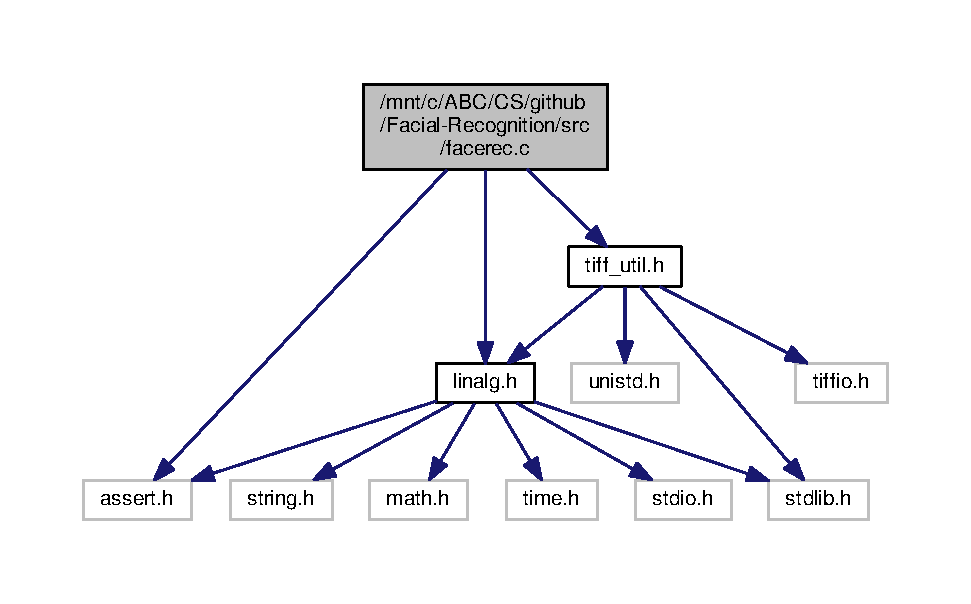
\includegraphics[width=350pt]{facerec_8c__incl}
\end{center}
\end{figure}
\subsection*{Functions}
\begin{DoxyCompactItemize}
\item 
\hypertarget{facerec_8c_ae66f6b31b5ad750f1fe042a706a4e3d4}{int {\bfseries main} ()}\label{facerec_8c_ae66f6b31b5ad750f1fe042a706a4e3d4}

\end{DoxyCompactItemize}


\subsection{Detailed Description}
File containing the main function. Minhyuk Park \begin{DoxyDate}{Date}
7 Nov 2017 
\end{DoxyDate}

\hypertarget{linalg_8c}{\section{/mnt/c/\-A\-B\-C/\-C\-S/github/\-Facial-\/\-Recognition/src/libs/linalg.c File Reference}
\label{linalg_8c}\index{/mnt/c/\-A\-B\-C/\-C\-S/github/\-Facial-\/\-Recognition/src/libs/linalg.\-c@{/mnt/c/\-A\-B\-C/\-C\-S/github/\-Facial-\/\-Recognition/src/libs/linalg.\-c}}
}


File containing common linear algebra functions.  


{\ttfamily \#include \char`\"{}linalg.\-h\char`\"{}}\\*
{\ttfamily \#include \char`\"{}tiff\-\_\-util.\-h\char`\"{}}\\*
Include dependency graph for linalg.\-c\-:
\nopagebreak
\begin{figure}[H]
\begin{center}
\leavevmode
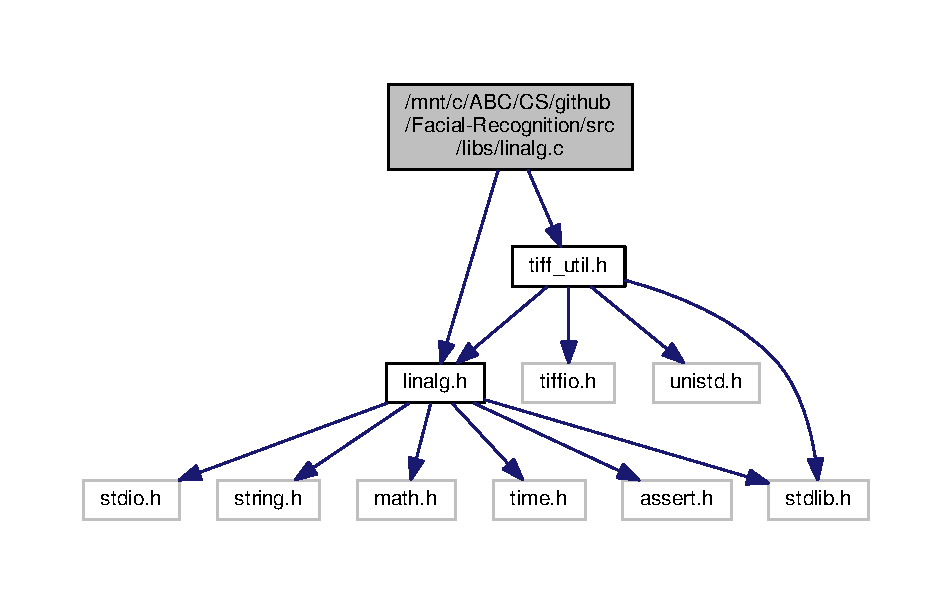
\includegraphics[width=350pt]{linalg_8c__incl}
\end{center}
\end{figure}
\subsection*{Functions}
\begin{DoxyCompactItemize}
\item 
\hyperlink{linalg_8h_a07a01529159cc35e78c1f7731ac7bda6}{vector} $\ast$ \hyperlink{linalg_8c_a7040be230e99648e77b0932600bf55ef}{vector\-\_\-create} (size\-\_\-t size)
\begin{DoxyCompactList}\small\item\em Creates a vector this function will malloc the exact space for the required dimensions. \end{DoxyCompactList}\item 
\hyperlink{linalg_8h_abc75382643898dd572498a574bf891c7}{matrix} $\ast$ \hyperlink{linalg_8c_a7821976cc30bc3131f3646bec1992d91}{matrix\-\_\-create} (size\-\_\-t row, size\-\_\-t col)
\begin{DoxyCompactList}\small\item\em Creates a matrix this function will malloc the exact space for the required dimensions. \end{DoxyCompactList}\item 
\hyperlink{linalg_8h_abc75382643898dd572498a574bf891c7}{matrix} $\ast$ \hyperlink{linalg_8c_a8a5d3412faa2267345b3a7d1ca6f58c1}{vec\-\_\-to\-\_\-mat} (\hyperlink{linalg_8h_a07a01529159cc35e78c1f7731ac7bda6}{vector} $\ast$vec, int orientation)
\begin{DoxyCompactList}\small\item\em Converts vector into matrix this function will \char`\"{}cast\char`\"{} the vector into a matrix by using the fact that they both have the same size. when calling this function, calling free() on the matrix will free the vector and vice versa. \end{DoxyCompactList}\item 
\hyperlink{linalg_8h_a07a01529159cc35e78c1f7731ac7bda6}{vector} $\ast$ \hyperlink{linalg_8c_a9059a420799b3aa9c04d5dd469523d91}{mat\-\_\-to\-\_\-vec} (\hyperlink{linalg_8h_abc75382643898dd572498a574bf891c7}{matrix} $\ast$mat)
\begin{DoxyCompactList}\small\item\em Converts matrix into vector this function will \char`\"{}cast\char`\"{} the matrix into a vector by using the fact that they both have the same size. when calling this function, calling free() on the vector will free the matrix and vice versa. the input matrix can only be a matrix with dimensions 1 X N (a row matrix) \end{DoxyCompactList}\item 
void \hyperlink{linalg_8c_a41ab46fdaa678c67aef38d873870a98d}{matrix\-\_\-reshape} (\hyperlink{linalg_8h_abc75382643898dd572498a574bf891c7}{matrix} $\ast$mat, size\-\_\-t row, size\-\_\-t col)
\begin{DoxyCompactList}\small\item\em Reshapes the matrix this function will reshape the matrix in constant time. \end{DoxyCompactList}\item 
double \hyperlink{linalg_8c_afc298e7d7d6a208e71ef073948b651d2}{dot\-\_\-product} (const double $\ast$left, const double $\ast$right, int length)
\begin{DoxyCompactList}\small\item\em Performs dot product on two double$\ast$ this function will malloc for the user a double arrays must be of same size. \end{DoxyCompactList}\item 
\hyperlink{linalg_8h_a07a01529159cc35e78c1f7731ac7bda6}{vector} $\ast$ \hyperlink{linalg_8c_a0c350b8673e50738602aa10cd6a86924}{vecscalar\-\_\-multiply} (const \hyperlink{linalg_8h_a07a01529159cc35e78c1f7731ac7bda6}{vector} $\ast$vec, const double scalar)
\begin{DoxyCompactList}\small\item\em Performs scalar multiplication of a vector this function will malloc for the user a vector$\ast$. \end{DoxyCompactList}\item 
\hyperlink{linalg_8h_a07a01529159cc35e78c1f7731ac7bda6}{vector} $\ast$ \hyperlink{linalg_8c_a2bc6dcc923c28a9d6f0ff38bd5de55f5}{vecscalar\-\_\-divide} (const \hyperlink{linalg_8h_a07a01529159cc35e78c1f7731ac7bda6}{vector} $\ast$vec, const double scalar)
\begin{DoxyCompactList}\small\item\em Performs scalar division of a vector this function will malloc for the user a vector$\ast$. \end{DoxyCompactList}\item 
\hyperlink{linalg_8h_a07a01529159cc35e78c1f7731ac7bda6}{vector} $\ast$ \hyperlink{linalg_8c_a4af2cd71186eeb14f970f97a27fbcef0}{vecmat\-\_\-multiply} (const \hyperlink{linalg_8h_a07a01529159cc35e78c1f7731ac7bda6}{vector} $\ast$vec, const \hyperlink{linalg_8h_abc75382643898dd572498a574bf891c7}{matrix} $\ast$mat)
\begin{DoxyCompactList}\small\item\em Performs vector matrix multiplication this function will malloc for the user a vector$\ast$ if the vector is of size M and the matrix size M by N, the resulting column vector will be of size N. \end{DoxyCompactList}\item 
\hyperlink{linalg_8h_a07a01529159cc35e78c1f7731ac7bda6}{vector} $\ast$ \hyperlink{linalg_8c_af88415d8996030537851e2c48d5337c4}{matvec\-\_\-multiply} (const \hyperlink{linalg_8h_abc75382643898dd572498a574bf891c7}{matrix} $\ast$mat, const \hyperlink{linalg_8h_a07a01529159cc35e78c1f7731ac7bda6}{vector} $\ast$vec)
\begin{DoxyCompactList}\small\item\em Performs matrix vector multiplication this function will malloc for the user a vector$\ast$ if the matrix is of size M by N and the vector N, the resulting row vector will be of size M. \end{DoxyCompactList}\item 
void \hyperlink{linalg_8c_a3c4e05af95e01c11963c912837d0d35b}{mat\-\_\-print} (const \hyperlink{linalg_8h_abc75382643898dd572498a574bf891c7}{matrix} $\ast$mat)
\begin{DoxyCompactList}\small\item\em prints the matrix this function will not modify the matrix and print to stdout \end{DoxyCompactList}\item 
void \hyperlink{linalg_8c_a1d2e72678bf82c44ba57020fc8588868}{vec\-\_\-print} (const \hyperlink{linalg_8h_a07a01529159cc35e78c1f7731ac7bda6}{vector} $\ast$vec)
\begin{DoxyCompactList}\small\item\em prints the vector this function will not modify the vector and print to stdout \end{DoxyCompactList}\item 
\hyperlink{linalg_8h_abc75382643898dd572498a574bf891c7}{matrix} $\ast$ \hyperlink{linalg_8c_a40a3d6442169157a458362f5e85c5843}{matmat\-\_\-multiply} (const \hyperlink{linalg_8h_abc75382643898dd572498a574bf891c7}{matrix} $\ast$left, const \hyperlink{linalg_8h_abc75382643898dd572498a574bf891c7}{matrix} $\ast$right)
\begin{DoxyCompactList}\small\item\em Performs standard matrix multiplication this function will malloc for the user a matrix$\ast$. \end{DoxyCompactList}\item 
\hyperlink{linalg_8h_abc75382643898dd572498a574bf891c7}{matrix} $\ast$ \hyperlink{linalg_8c_a9d1ca6441796b3d9c53f2a2923dc06c7}{matmat\-\_\-addition} (const \hyperlink{linalg_8h_abc75382643898dd572498a574bf891c7}{matrix} $\ast$left, const \hyperlink{linalg_8h_abc75382643898dd572498a574bf891c7}{matrix} $\ast$right)
\begin{DoxyCompactList}\small\item\em Performs standard matrix addition this function will malloc for the user a matrix$\ast$. \end{DoxyCompactList}\item 
\hyperlink{linalg_8h_abc75382643898dd572498a574bf891c7}{matrix} $\ast$ \hyperlink{linalg_8c_a6b7138d5fae752feceeb9faea996cb54}{matmat\-\_\-subtraction} (const \hyperlink{linalg_8h_abc75382643898dd572498a574bf891c7}{matrix} $\ast$left, const \hyperlink{linalg_8h_abc75382643898dd572498a574bf891c7}{matrix} $\ast$right)
\begin{DoxyCompactList}\small\item\em Performs standard matrix subtration this function will malloc for the user a matrix$\ast$. \end{DoxyCompactList}\item 
\hyperlink{linalg_8h_abc75382643898dd572498a574bf891c7}{matrix} $\ast$ \hyperlink{linalg_8c_a32cb81b161008e2b1fd862ae9d45caa2}{matscalar\-\_\-multiply} (const \hyperlink{linalg_8h_abc75382643898dd572498a574bf891c7}{matrix} $\ast$mat, const double scalar)
\begin{DoxyCompactList}\small\item\em Performs scalar multiplication of a matrix this function will malloc for the user a matrix$\ast$. \end{DoxyCompactList}\item 
\hyperlink{linalg_8h_abc75382643898dd572498a574bf891c7}{matrix} $\ast$ \hyperlink{linalg_8c_a98269f4c3f77b32dc52e30108713cb28}{matscalar\-\_\-divide} (const \hyperlink{linalg_8h_abc75382643898dd572498a574bf891c7}{matrix} $\ast$mat, const double scalar)
\begin{DoxyCompactList}\small\item\em Performs scalar division of a matrix this function will malloc for the user a matrix$\ast$. \end{DoxyCompactList}\item 
\hyperlink{linalg_8h_abc75382643898dd572498a574bf891c7}{matrix} $\ast$ \hyperlink{linalg_8c_a2ac4400497d3a421f3f631d6329010b6}{mat\-\_\-transpose} (const \hyperlink{linalg_8h_abc75382643898dd572498a574bf891c7}{matrix} $\ast$mat)
\begin{DoxyCompactList}\small\item\em Performs matrix transpose this function will malloc for the user a matrix$\ast$. \end{DoxyCompactList}\item 
void \hyperlink{linalg_8c_adbfad21fe7e851455d625173e67b8504}{vec\-\_\-append} (\hyperlink{linalg_8h_a07a01529159cc35e78c1f7731ac7bda6}{vector} $\ast$$\ast$vec\-\_\-a, \hyperlink{linalg_8h_a07a01529159cc35e78c1f7731ac7bda6}{vector} $\ast$vec\-\_\-b)
\begin{DoxyCompactList}\small\item\em Appends vector b to vector a this function will realloc for the user vector a and free vector b. \end{DoxyCompactList}\item 
void \hyperlink{linalg_8c_a5a1e9091382fa5e859255c55177ec401}{eigen} (int n, double a\mbox{[}$\,$\mbox{]}, int it\-\_\-max, double v\mbox{[}$\,$\mbox{]}, double d\mbox{[}$\,$\mbox{]}, int $\ast$it\-\_\-num, int $\ast$rot\-\_\-num)
\begin{DoxyCompactList}\small\item\em Performs Jacobi eigenvalue iteration this function will required the user to pass in non-\/null it\-\_\-num and rot\-\_\-num it does not malloc but rather requires the caller to malloc space for it. \end{DoxyCompactList}\item 
void \hyperlink{linalg_8c_a97f97bfa6f100928e8d6c9f085bd9d12}{mat\-\_\-identity} (int n, double a\mbox{[}$\,$\mbox{]})
\begin{DoxyCompactList}\small\item\em modifies a matrix to be the identity matrix of size n \end{DoxyCompactList}\item 
void \hyperlink{linalg_8c_abc4918a0c6b295404ebfadfe78b26bdd}{diag\-\_\-vector} (int n, double a\mbox{[}$\,$\mbox{]}, double v\mbox{[}$\,$\mbox{]})
\begin{DoxyCompactList}\small\item\em gets the diagonal entries \end{DoxyCompactList}\item 
double \hyperlink{linalg_8c_a948f2b3da29647be0bcb62e717dfec2d}{frobenius\-\_\-norm} (int n, int k, double a\mbox{[}$\,$\mbox{]}, double x\mbox{[}$\,$\mbox{]}, double lambda\mbox{[}$\,$\mbox{]})
\begin{DoxyCompactList}\small\item\em computes the Frobenius norm in a right eigensystem \end{DoxyCompactList}\item 
\hyperlink{linalg_8h_abc75382643898dd572498a574bf891c7}{matrix} $\ast$ \hyperlink{linalg_8c_ad41ec0281d3766f40963b77520ce600d}{covmat} (\hyperlink{linalg_8h_abc75382643898dd572498a574bf891c7}{matrix} $\ast$mat)
\begin{DoxyCompactList}\small\item\em computes the variance covariance matrix \end{DoxyCompactList}\item 
\hyperlink{linalg_8h_a07a01529159cc35e78c1f7731ac7bda6}{vector} $\ast$ \hyperlink{linalg_8c_a71f490da601d057f4ce45efb9a48c2ae}{compute\-\_\-average} (\hyperlink{linalg_8h_abc75382643898dd572498a574bf891c7}{matrix} $\ast$images, int num\-\_\-images)
\begin{DoxyCompactList}\small\item\em computes the average matrix of all the $\ast$vector images \end{DoxyCompactList}\end{DoxyCompactItemize}


\subsection{Detailed Description}
File containing common linear algebra functions. Minhyuk Park \begin{DoxyDate}{Date}
7 Nov 2017 
\end{DoxyDate}


\subsection{Function Documentation}
\hypertarget{linalg_8c_a71f490da601d057f4ce45efb9a48c2ae}{\index{linalg.\-c@{linalg.\-c}!compute\-\_\-average@{compute\-\_\-average}}
\index{compute\-\_\-average@{compute\-\_\-average}!linalg.c@{linalg.\-c}}
\subsubsection[{compute\-\_\-average}]{\setlength{\rightskip}{0pt plus 5cm}{\bf vector}$\ast$ compute\-\_\-average (
\begin{DoxyParamCaption}
\item[{{\bf matrix} $\ast$}]{images, }
\item[{int}]{num\-\_\-images}
\end{DoxyParamCaption}
)}}\label{linalg_8c_a71f490da601d057f4ce45efb9a48c2ae}


computes the average matrix of all the $\ast$vector images 

\begin{DoxyReturn}{Returns}
vector$\ast$ the average image 
\end{DoxyReturn}

\begin{DoxyParams}{Parameters}
{\em images} & matrix$\ast$ a matrix where each column represents an image \\
\hline
{\em num\-\_\-images} & int number of images in the vector \\
\hline
\end{DoxyParams}


References M\-A\-T, \-\_\-matrix\-::row, \-\_\-vector\-::size, V\-E\-C, and vector\-\_\-create().


\begin{DoxyCode}
407                                                         \{
408     \textcolor{comment}{/*}
409 \textcolor{comment}{    matrix* ones\_row = matrix\_create(1, num\_images);
}
410 \textcolor{comment}{    for(int i =0; i <num\_images; i++) \{
}
411 \textcolor{comment}{        MAT(ones\_row, 0,i) = 1;
}
412 \textcolor{comment}{    \}
}
413 \textcolor{comment}{    matrix* row\_images = mat\_transpose(images);
}
414 \textcolor{comment}{    matrix* row\_sum = matmat\_multiply(ones\_row, row\_images);
}
415 \textcolor{comment}{    vector* vector\_row\_sum = mat\_to\_vec(row\_sum);
}
416 \textcolor{comment}{    vector* img\_avg = vecscalar\_divide(vector\_row\_sum, num\_images);
}
417 \textcolor{comment}{    free(vector\_row\_sum);
}
418 \textcolor{comment}{    free(row\_images);
}
419 \textcolor{comment}{    free(ones\_row);
}
420 \textcolor{comment}{    */}
421     \hyperlink{struct__vector}{vector}* img\_avg = \hyperlink{linalg_8c_a7040be230e99648e77b0932600bf55ef}{vector\_create}(images->\hyperlink{struct__matrix_a1087bec6a11b0773b4852c4ca49fc32a}{row});
422 
423     \textcolor{keywordflow}{for}(\textcolor{keywordtype}{size\_t} i = 0; i < img\_avg->\hyperlink{struct__vector_a1ed8dca78f3e589deb8dad9b53aec3fa}{size}; i ++) \{
424         uint32 avg\_pixel = 0;
425 
426         uint32 r = 0;
427         uint32 g = 0;
428         uint32 b = 0;
429         uint32 a = 0;
430         \textcolor{keywordflow}{for}(\textcolor{keywordtype}{int} j = 0; j < num\_images; j ++) \{
431             uint32 current\_pixel = \hyperlink{linalg_8h_ae0e32e641b8137c777d52988864296e3}{MAT}(images, i, j);
432 
433             r += ((current\_pixel & 0xff) * (current\_pixel & 0xff));
434             g += (((current\_pixel >> 8) & 0xff) * ((current\_pixel >> 8) & 0xff));
435             b += (((current\_pixel >> 16) & 0xff) * ((current\_pixel >> 16) & 0xff));
436             a += (((current\_pixel >> 24) & 0xff) * ((current\_pixel >> 24) & 0xff));
437         \}
438 
439         r /= num\_images;
440         g /= num\_images;
441         b /= num\_images;
442         a /= num\_images;
443 
444         r = sqrt(r);
445         g = sqrt(g);
446         b = sqrt(b);
447         a = sqrt(a);
448         \textcolor{comment}{/*}
449 \textcolor{comment}{        for(int j = 0; j < num\_images; j ++) \{
}
450 \textcolor{comment}{            uint32 current\_pixel = MAT(images, i, j);
}
451 \textcolor{comment}{}
452 \textcolor{comment}{            r += ((current\_pixel & 0xff));
}
453 \textcolor{comment}{            g += (((current\_pixel >> 8) & 0xff));
}
454 \textcolor{comment}{            b += (((current\_pixel >> 16) & 0xff));
}
455 \textcolor{comment}{            a += (((current\_pixel >> 24) & 0xff));
}
456 \textcolor{comment}{        \}
}
457 \textcolor{comment}{}
458 \textcolor{comment}{        r /= num\_images;
}
459 \textcolor{comment}{        g /= num\_images;
}
460 \textcolor{comment}{        b /= num\_images;
}
461 \textcolor{comment}{        a /= num\_images;
}
462 \textcolor{comment}{        */}
463 
464 
465         avg\_pixel |= r;
466         avg\_pixel |= (g << 8);
467         avg\_pixel |= (b << 16);
468         avg\_pixel |= (a << 24);
469 
470         \hyperlink{linalg_8h_a03e904294c904b01194a25323fc2f6ec}{VEC}(img\_avg, i) = avg\_pixel;
471     \}
472 
473 
474     
475 
476     \textcolor{keywordflow}{return} img\_avg;
477 \}
\end{DoxyCode}
\hypertarget{linalg_8c_ad41ec0281d3766f40963b77520ce600d}{\index{linalg.\-c@{linalg.\-c}!covmat@{covmat}}
\index{covmat@{covmat}!linalg.c@{linalg.\-c}}
\subsubsection[{covmat}]{\setlength{\rightskip}{0pt plus 5cm}{\bf matrix}$\ast$ covmat (
\begin{DoxyParamCaption}
\item[{{\bf matrix} $\ast$}]{mat}
\end{DoxyParamCaption}
)}}\label{linalg_8c_ad41ec0281d3766f40963b77520ce600d}


computes the variance covariance matrix 

\begin{DoxyReturn}{Returns}
matrix$\ast$ the output variance-\/covariance matrix this function will malloc a new matrix 
\end{DoxyReturn}

\begin{DoxyParams}{Parameters}
{\em mat} & a matrix$\ast$ representing the input matrix of deviation scores of size n by k \\
\hline
\end{DoxyParams}


References mat\-\_\-transpose(), matmat\-\_\-multiply(), matscalar\-\_\-divide(), and \-\_\-matrix\-::row.


\begin{DoxyCode}
397                             \{
398     \textcolor{keywordtype}{size\_t} n = mat->\hyperlink{struct__matrix_a1087bec6a11b0773b4852c4ca49fc32a}{row};
399     \hyperlink{struct__matrix}{matrix}* mat\_T = \hyperlink{linalg_8c_a2ac4400497d3a421f3f631d6329010b6}{mat\_transpose}(mat);
400     \hyperlink{struct__matrix}{matrix}* x\_T\_x = \hyperlink{linalg_8c_a40a3d6442169157a458362f5e85c5843}{matmat\_multiply}(mat\_T, mat);
401     \hyperlink{struct__matrix}{matrix}* retmat = \hyperlink{linalg_8c_a98269f4c3f77b32dc52e30108713cb28}{matscalar\_divide}(x\_T\_x, n);
402     free(x\_T\_x);
403     free(mat\_T);
404     \textcolor{keywordflow}{return} retmat;
405 \}
\end{DoxyCode}
\hypertarget{linalg_8c_abc4918a0c6b295404ebfadfe78b26bdd}{\index{linalg.\-c@{linalg.\-c}!diag\-\_\-vector@{diag\-\_\-vector}}
\index{diag\-\_\-vector@{diag\-\_\-vector}!linalg.c@{linalg.\-c}}
\subsubsection[{diag\-\_\-vector}]{\setlength{\rightskip}{0pt plus 5cm}void diag\-\_\-vector (
\begin{DoxyParamCaption}
\item[{int}]{n, }
\item[{double}]{a\mbox{[}$\,$\mbox{]}, }
\item[{double}]{v\mbox{[}$\,$\mbox{]}}
\end{DoxyParamCaption}
)}}\label{linalg_8c_abc4918a0c6b295404ebfadfe78b26bdd}


gets the diagonal entries 


\begin{DoxyParams}{Parameters}
{\em n} & int the dimension \\
\hline
{\em a\mbox{[}$\,$\mbox{]}} & double\mbox{[}\mbox{]} input the matrix, N by N \\
\hline
{\em v\mbox{[}$\,$\mbox{]}} & double\mbox{[}\mbox{]} output the diagonal entries, N \\
\hline
\end{DoxyParams}


Referenced by eigen().


\begin{DoxyCode}
363                                                 \{
364     \textcolor{keywordflow}{for}(\textcolor{keywordtype}{int} i = 0; i < n; i ++) \{
365         v[i] = a[i + i * n];
366     \}
367     \textcolor{keywordflow}{return};
368 \}
\end{DoxyCode}
\hypertarget{linalg_8c_afc298e7d7d6a208e71ef073948b651d2}{\index{linalg.\-c@{linalg.\-c}!dot\-\_\-product@{dot\-\_\-product}}
\index{dot\-\_\-product@{dot\-\_\-product}!linalg.c@{linalg.\-c}}
\subsubsection[{dot\-\_\-product}]{\setlength{\rightskip}{0pt plus 5cm}double dot\-\_\-product (
\begin{DoxyParamCaption}
\item[{const double $\ast$}]{left, }
\item[{const double $\ast$}]{right, }
\item[{int}]{length}
\end{DoxyParamCaption}
)}}\label{linalg_8c_afc298e7d7d6a208e71ef073948b651d2}


Performs dot product on two double$\ast$ this function will malloc for the user a double arrays must be of same size. 

\begin{DoxyReturn}{Returns}
a double representing the inner product 
\end{DoxyReturn}

\begin{DoxyParams}{Parameters}
{\em left} & const double$\ast$ the first vector \\
\hline
{\em right} & const double$\ast$ the second vector \\
\hline
{\em length} & int the size of the vectors \\
\hline
\end{DoxyParams}


Referenced by matvec\-\_\-multiply().


\begin{DoxyCode}
57                                                                         \{
58     \textcolor{keywordtype}{double} retval = 0.0;
59     \textcolor{keywordflow}{for}(\textcolor{keywordtype}{int} i = 0; i < length; i ++) \{
60         retval += (left[i] * right[i]);
61     \}
62     \textcolor{keywordflow}{return} retval;
63 \}
\end{DoxyCode}
\hypertarget{linalg_8c_a5a1e9091382fa5e859255c55177ec401}{\index{linalg.\-c@{linalg.\-c}!eigen@{eigen}}
\index{eigen@{eigen}!linalg.c@{linalg.\-c}}
\subsubsection[{eigen}]{\setlength{\rightskip}{0pt plus 5cm}void eigen (
\begin{DoxyParamCaption}
\item[{int}]{N, }
\item[{double}]{a\mbox{[}$\,$\mbox{]}, }
\item[{int}]{it\-\_\-max, }
\item[{double}]{v\mbox{[}$\,$\mbox{]}, }
\item[{double}]{d\mbox{[}$\,$\mbox{]}, }
\item[{int $\ast$}]{it\-\_\-num, }
\item[{int $\ast$}]{rot\-\_\-num}
\end{DoxyParamCaption}
)}}\label{linalg_8c_a5a1e9091382fa5e859255c55177ec401}


Performs Jacobi eigenvalue iteration this function will required the user to pass in non-\/null it\-\_\-num and rot\-\_\-num it does not malloc but rather requires the caller to malloc space for it. 


\begin{DoxyParams}{Parameters}
{\em N} & int the dimiension of the input matrix a, which is a N by N matrix \\
\hline
{\em a\mbox{[}$\,$\mbox{]}} & double\mbox{[}\mbox{]} the input matrix which has to be square, real, and symmetric \\
\hline
{\em it\-\_\-max} & int maximum number of iterations to stop at \\
\hline
{\em v\mbox{[}$\,$\mbox{]}} & double\mbox{[}\mbox{]}output matrix of eigenvectors, which is a N by N matrix \\
\hline
{\em d\mbox{[}$\,$\mbox{]}} & double\mbox{[}\mbox{]} output matrix of eigenvalues, in descending order \\
\hline
{\em it\-\_\-num} & int$\ast$ output total number of iterations \\
\hline
{\em rot\-\_\-num} & int$\ast$ output total number of rotations \\
\hline
\end{DoxyParams}


References diag\-\_\-vector(), and mat\-\_\-identity().


\begin{DoxyCode}
212                                                                                              \{
213     \hyperlink{linalg_8c_a97f97bfa6f100928e8d6c9f085bd9d12}{mat\_identity}(n, v); \textcolor{comment}{// create the identity matrix using what the caller allocated for us}
214     \hyperlink{linalg_8c_abc4918a0c6b295404ebfadfe78b26bdd}{diag\_vector}(n, a, d); \textcolor{comment}{// get the diagonal values of a and store it in caller allocated
       vector d}
215 
216     \textcolor{keywordtype}{double}* bw = (\textcolor{keywordtype}{double}*) malloc(n * \textcolor{keyword}{sizeof}(\textcolor{keywordtype}{double}));
217     \textcolor{keywordtype}{double}* zw = (\textcolor{keywordtype}{double}*) malloc(n * \textcolor{keyword}{sizeof}(\textcolor{keywordtype}{double}));
218 
219     \textcolor{keywordflow}{for}(\textcolor{keywordtype}{int} i = 0; i < n; i ++) \{
220         bw[i] = d[i];
221         zw[i] = 0.0;
222     \}
223     *it\_num = 0;
224     *rot\_num = 0;
225 
226     \textcolor{keywordtype}{double} thresh = 0.0;
227     \textcolor{keywordtype}{double} gapq = 0.0;
228     \textcolor{keywordflow}{while}(*it\_num < it\_max) \{
229         *it\_num += 1;
230         thresh = 0.0;
231         \textcolor{comment}{// set up the convergence threshold}
232         \textcolor{comment}{// based on the size of strict upper triangle}
233         \textcolor{keywordflow}{for}(\textcolor{keywordtype}{int} i = 0; i < n; i ++) \{
234             \textcolor{keywordflow}{for}(\textcolor{keywordtype}{int} j = 0; j < i; j ++) \{
235                 thresh += (a[j + i * n] * a[j + i * n]);
236             \}
237         \}
238         \textcolor{comment}{// PASS 1}
239         thresh = sqrt(thresh) / (double)(4 * n);
240         \textcolor{keywordflow}{if}(thresh == 0.0) \{
241             \textcolor{keywordflow}{break};
242         \}
243         \textcolor{comment}{// PASS 2}
244         \textcolor{keywordflow}{for}(\textcolor{keywordtype}{int} p = 0; p < n; p ++) \{
245             \textcolor{keywordflow}{for}(\textcolor{keywordtype}{int} q = p + 1; q < n; q ++) \{
246                 gapq = 10.0 * fabs(a[p + q * n]);
247                 \textcolor{keywordtype}{double} termp = gapq + fabs(d[p]);
248                 \textcolor{keywordtype}{double} termq = gapq + fabs(d[q]);
249                 \textcolor{keywordflow}{if}(4 < *it\_num && termp == fabs(d[p]) && termq == fabs(d[q])) \{
250                     a[p + q * n] = 0.0;
251                 \textcolor{comment}{// apply rotation otherwise}
252                 \textcolor{comment}{// PASS 3}
253                 \} \textcolor{keywordflow}{else} \textcolor{keywordflow}{if}(thresh <= fabs(a[p + q * n])) \{
254                     \textcolor{keywordtype}{double} h = d[q] - d[p];
255                     \textcolor{keywordtype}{double} term = fabs(h) + gapq;
256                     \textcolor{keywordtype}{double} t = 0.0;
257                     \textcolor{keywordflow}{if}(term == fabs(h)) \{
258                         t = a[p + q * n] / h;
259                     \} \textcolor{keywordflow}{else} \{
260                         \textcolor{keywordtype}{double} theta = 0.5 * h / a[p + q * n];
261                         t = 1.0 / (fabs(theta) + sqrt(1.0 + theta * theta));
262                         \textcolor{keywordflow}{if}(theta < 0.0) \{
263                             t = -t;
264                         \}
265                     \}
266                     \textcolor{comment}{// PASS 4}
267                     \textcolor{keywordtype}{double} c = 1.0 / sqrt(1.0 + t * t);
268                     \textcolor{keywordtype}{double} s = t * c;
269                     \textcolor{keywordtype}{double} tau = s / (1.0 + c);
270                     h = t * a[p + q * n];
271 
272                     zw[p] -= h;
273                     zw[q] += h;
274                     d[p] -= h;
275                     d[q] += h;
276                     a[p + q * n] = 0.0;
277                     \textcolor{comment}{// PASS 5}
278                     \textcolor{comment}{// rotate}
279                     \textcolor{keywordtype}{double} g = 0.0;
280                     \textcolor{keywordflow}{for}(\textcolor{keywordtype}{int} j = 0; j < p; j ++) \{
281                         g = a[j + p * n];
282                         h = a[j + q * n];
283                         a[j + p * n] = g - s * (h + g * tau);
284                         a[j + q * n] = h + s * (g - h * tau);
285                     \}
286                     \textcolor{keywordflow}{for}(\textcolor{keywordtype}{int} j = p + 1; j < q; j ++) \{
287                         g = a[p + j * n];
288                         h = a[j + q * n];
289                         a[p + j * n] = g - s * (h + g * tau);
290                         a[j + q * n] = h + s * (g - h * tau);
291                     \}
292                     \textcolor{keywordflow}{for}(\textcolor{keywordtype}{int} j = q + 1; j < n; j ++) \{
293                         g = a[p + j * n];
294                         h = a[q + j * n];
295                         a[p + j * n] = g - s * (h + g * tau);
296                         a[q + j * n] = h + s * (g - h * tau);
297                     \}
298                     \textcolor{comment}{// PASS 6}
299                     \textcolor{comment}{// store to eigenvector matrix v}
300                     \textcolor{keywordflow}{for}(\textcolor{keywordtype}{int} j = 0; j < n; j ++) \{
301                         g = v[j + p * n];
302                         h = v[j + q * n];
303                         v[j + p * n] = g - s * (h + g * tau);
304                         v[j + q * n] = h + s * (g - h * tau);
305                     \}
306                     *rot\_num += 1;
307                 \}
308             \}
309         \}
310         \textcolor{keywordflow}{for}(\textcolor{keywordtype}{int} i = 0; i < n; i ++) \{
311             bw[i] += zw[i];
312             d[i] = bw[i];
313             zw[i] = 0.0;
314         \}
315     \}
316     \textcolor{comment}{// PASS 7}
317     \textcolor{comment}{// restore upper triangle}
318     \textcolor{keywordflow}{for}(\textcolor{keywordtype}{int} i = 0; i < n; i ++) \{
319         \textcolor{keywordflow}{for}(\textcolor{keywordtype}{int} j = 0; j < i; j ++) \{
320             a[j + i * n] = a [i + j * n];
321         \}
322     \}
323     \textcolor{keywordflow}{for}(\textcolor{keywordtype}{int} k = 0; k < n - 1; k ++) \{
324         \textcolor{keywordtype}{int} m = k;
325         \textcolor{keywordflow}{for}(\textcolor{keywordtype}{int} l = k + 1; l < n; l ++) \{
326             \textcolor{keywordflow}{if}(d[l] < d[m]) \{
327                 m = l;
328             \}
329         \}
330         \textcolor{keywordflow}{if}(m != k) \{
331             \textcolor{keywordtype}{double} t = d[m];
332             d[m] = d[k];
333             d[k] = t;
334             \textcolor{keywordflow}{for}(\textcolor{keywordtype}{int} i = 0; i < n; i ++) \{
335                 \textcolor{keywordtype}{double} w = v[i + m * n];
336                 v[i + m * n] = v[i + k * n];
337                 v[i + k * n] = w;
338             \}
339         \}
340     \}
341     free(bw);
342     free(zw);
343     \textcolor{keywordflow}{return};
344 \}
\end{DoxyCode}
\hypertarget{linalg_8c_a948f2b3da29647be0bcb62e717dfec2d}{\index{linalg.\-c@{linalg.\-c}!frobenius\-\_\-norm@{frobenius\-\_\-norm}}
\index{frobenius\-\_\-norm@{frobenius\-\_\-norm}!linalg.c@{linalg.\-c}}
\subsubsection[{frobenius\-\_\-norm}]{\setlength{\rightskip}{0pt plus 5cm}double frobenius\-\_\-norm (
\begin{DoxyParamCaption}
\item[{int}]{n, }
\item[{int}]{k, }
\item[{double}]{a\mbox{[}$\,$\mbox{]}, }
\item[{double}]{x\mbox{[}$\,$\mbox{]}, }
\item[{double}]{lambda\mbox{[}$\,$\mbox{]}}
\end{DoxyParamCaption}
)}}\label{linalg_8c_a948f2b3da29647be0bcb62e717dfec2d}


computes the Frobenius norm in a right eigensystem 

\begin{DoxyReturn}{Returns}
double the frobenius norm of A $\ast$ X -\/ X $\ast$ lambda 
\end{DoxyReturn}

\begin{DoxyParams}{Parameters}
{\em n} & int the dimension of the matrix \\
\hline
{\em k} & int the number of eigen vectors \\
\hline
{\em a\mbox{[}$\,$\mbox{]}} & double\mbox{[}\mbox{]} input matrix of size n by n \\
\hline
{\em x\mbox{[}$\,$\mbox{]}} & double\mbox{[}\mbox{]} input vector of eigenvectors of size k \\
\hline
{\em lamdba\mbox{[}$\,$\mbox{]}} & double\mbox{[}\mbox{]} input vector of eigen values \\
\hline
\end{DoxyParams}

\begin{DoxyCode}
371                                                                              \{
372     \textcolor{keywordtype}{double}* c = (\textcolor{keywordtype}{double}*) malloc(n * k * \textcolor{keyword}{sizeof}(\textcolor{keywordtype}{double}));
373     \textcolor{keywordflow}{for}(\textcolor{keywordtype}{int} i = 0; i < k; i ++) \{
374         \textcolor{keywordflow}{for}(\textcolor{keywordtype}{int} j = 0; j < n; j ++) \{
375             c[j + i * n] = 0.0;
376             \textcolor{keywordflow}{for}(\textcolor{keywordtype}{int} l = 0; l < n; l ++) \{
377                 c[j + i * n] = c[j + i * n] + a[j + l * n] * x[l + i * n];
378             \}
379         \}
380     \}
381     \textcolor{keywordflow}{for}(\textcolor{keywordtype}{int} i = 0; i < k; i ++) \{
382         \textcolor{keywordflow}{for}(\textcolor{keywordtype}{int} j = 0; j < n; j ++) \{
383             c[j + i * n] = c[j + i * n] - lambda[i] * x[j + i * n];
384         \}
385     \}
386     \textcolor{keywordtype}{double} retval = 0.0;
387     \textcolor{keywordflow}{for}(\textcolor{keywordtype}{int} i = 0; i < k; i ++) \{
388         \textcolor{keywordflow}{for}(\textcolor{keywordtype}{int} j = 0; j < n; j ++) \{
389             retval += pow(c[j + i * n], 2);
390         \}
391     \}
392     retval = sqrt(retval);
393     free(c);
394     \textcolor{keywordflow}{return} retval;
395 \}
\end{DoxyCode}
\hypertarget{linalg_8c_a97f97bfa6f100928e8d6c9f085bd9d12}{\index{linalg.\-c@{linalg.\-c}!mat\-\_\-identity@{mat\-\_\-identity}}
\index{mat\-\_\-identity@{mat\-\_\-identity}!linalg.c@{linalg.\-c}}
\subsubsection[{mat\-\_\-identity}]{\setlength{\rightskip}{0pt plus 5cm}void mat\-\_\-identity (
\begin{DoxyParamCaption}
\item[{int}]{n, }
\item[{double}]{a\mbox{[}$\,$\mbox{]}}
\end{DoxyParamCaption}
)}}\label{linalg_8c_a97f97bfa6f100928e8d6c9f085bd9d12}


modifies a matrix to be the identity matrix of size n 


\begin{DoxyParams}{Parameters}
{\em n} & int the dimension \\
\hline
{\em a\mbox{[}$\,$\mbox{]}} & double output identity matrix \\
\hline
\end{DoxyParams}


Referenced by eigen().


\begin{DoxyCode}
347                                      \{
348     \textcolor{keywordtype}{int} k = 0;
349     \textcolor{keywordflow}{for} (\textcolor{keywordtype}{int} j = 0; j < n; j ++ ) \{
350         \textcolor{keywordflow}{for} (\textcolor{keywordtype}{int} i = 0; i < n; i ++ ) \{
351             \textcolor{keywordflow}{if} ( i == j ) \{
352                 a[k] = 1.0;
353             \} \textcolor{keywordflow}{else} \{
354                 a[k] = 0.0;
355             \}
356             k += 1;
357         \}
358     \}
359     \textcolor{keywordflow}{return};
360 \}
\end{DoxyCode}
\hypertarget{linalg_8c_a3c4e05af95e01c11963c912837d0d35b}{\index{linalg.\-c@{linalg.\-c}!mat\-\_\-print@{mat\-\_\-print}}
\index{mat\-\_\-print@{mat\-\_\-print}!linalg.c@{linalg.\-c}}
\subsubsection[{mat\-\_\-print}]{\setlength{\rightskip}{0pt plus 5cm}void mat\-\_\-print (
\begin{DoxyParamCaption}
\item[{const {\bf matrix} $\ast$}]{mat}
\end{DoxyParamCaption}
)}}\label{linalg_8c_a3c4e05af95e01c11963c912837d0d35b}


prints the matrix this function will not modify the matrix and print to stdout 


\begin{DoxyParams}{Parameters}
{\em mat} & const matrix$\ast$ the matrix to be printed \\
\hline
\end{DoxyParams}


References \-\_\-matrix\-::col, M\-A\-T, and \-\_\-matrix\-::row.


\begin{DoxyCode}
107                                   \{
108     \textcolor{keywordflow}{for}(\textcolor{keywordtype}{size\_t} i = 0; i < mat->\hyperlink{struct__matrix_a1087bec6a11b0773b4852c4ca49fc32a}{row}; i ++) \{
109         \textcolor{keywordflow}{for}(\textcolor{keywordtype}{size\_t} j = 0; j < mat->\hyperlink{struct__matrix_a7e9feb52cfc0a9d7cba5320abcaa997a}{col}; j ++) \{
110             \textcolor{keywordflow}{if}(j == mat->\hyperlink{struct__matrix_a7e9feb52cfc0a9d7cba5320abcaa997a}{col} - 1) \{
111                 printf(\textcolor{stringliteral}{"%f "}, \hyperlink{linalg_8h_ae0e32e641b8137c777d52988864296e3}{MAT}(mat, i, j));                
112             \} \textcolor{keywordflow}{else} \{
113                 printf(\textcolor{stringliteral}{"%f, "}, \hyperlink{linalg_8h_ae0e32e641b8137c777d52988864296e3}{MAT}(mat, i, j));
114             \}
115         \}
116         printf(\textcolor{stringliteral}{"\(\backslash\)n"});
117     \}
118 \}
\end{DoxyCode}
\hypertarget{linalg_8c_a9059a420799b3aa9c04d5dd469523d91}{\index{linalg.\-c@{linalg.\-c}!mat\-\_\-to\-\_\-vec@{mat\-\_\-to\-\_\-vec}}
\index{mat\-\_\-to\-\_\-vec@{mat\-\_\-to\-\_\-vec}!linalg.c@{linalg.\-c}}
\subsubsection[{mat\-\_\-to\-\_\-vec}]{\setlength{\rightskip}{0pt plus 5cm}{\bf vector}$\ast$ mat\-\_\-to\-\_\-vec (
\begin{DoxyParamCaption}
\item[{{\bf matrix} $\ast$}]{mat}
\end{DoxyParamCaption}
)}}\label{linalg_8c_a9059a420799b3aa9c04d5dd469523d91}


Converts matrix into vector this function will \char`\"{}cast\char`\"{} the matrix into a vector by using the fact that they both have the same size. when calling this function, calling free() on the vector will free the matrix and vice versa. the input matrix can only be a matrix with dimensions 1 X N (a row matrix) 

\begin{DoxyReturn}{Returns}
vector$\ast$ the new pointer for input matrix$\ast$ 
\end{DoxyReturn}

\begin{DoxyParams}{Parameters}
{\em mat} & matrix$\ast$ to be converted in terms of the newly formed vector \\
\hline
\end{DoxyParams}


References \-\_\-matrix\-::col, and \-\_\-matrix\-::row.


\begin{DoxyCode}
43                                 \{
44     assert(mat->\hyperlink{struct__matrix_a1087bec6a11b0773b4852c4ca49fc32a}{row} = 1);
45     mat->\hyperlink{struct__matrix_a1087bec6a11b0773b4852c4ca49fc32a}{row} = mat->\hyperlink{struct__matrix_a7e9feb52cfc0a9d7cba5320abcaa997a}{col};
46     mat->\hyperlink{struct__matrix_a7e9feb52cfc0a9d7cba5320abcaa997a}{col} = 1;
47     \textcolor{keywordflow}{return} (\hyperlink{struct__vector}{vector}*)mat;
48 \}
\end{DoxyCode}
\hypertarget{linalg_8c_a2ac4400497d3a421f3f631d6329010b6}{\index{linalg.\-c@{linalg.\-c}!mat\-\_\-transpose@{mat\-\_\-transpose}}
\index{mat\-\_\-transpose@{mat\-\_\-transpose}!linalg.c@{linalg.\-c}}
\subsubsection[{mat\-\_\-transpose}]{\setlength{\rightskip}{0pt plus 5cm}{\bf matrix}$\ast$ mat\-\_\-transpose (
\begin{DoxyParamCaption}
\item[{const {\bf matrix} $\ast$}]{mat}
\end{DoxyParamCaption}
)}}\label{linalg_8c_a2ac4400497d3a421f3f631d6329010b6}


Performs matrix transpose this function will malloc for the user a matrix$\ast$. 

\begin{DoxyReturn}{Returns}
matrix$\ast$ the newly transposed and malloced matrix 
\end{DoxyReturn}

\begin{DoxyParams}{Parameters}
{\em mat} & const matrix$\ast$ the matrix to be transposed \\
\hline
\end{DoxyParams}


References \-\_\-matrix\-::col, M\-A\-T, matrix\-\_\-create(), and \-\_\-matrix\-::row.



Referenced by covmat().


\begin{DoxyCode}
181                                          \{
182     \hyperlink{struct__matrix}{matrix}* retval = \hyperlink{linalg_8c_a7821976cc30bc3131f3646bec1992d91}{matrix\_create}(mat->\hyperlink{struct__matrix_a7e9feb52cfc0a9d7cba5320abcaa997a}{col}, mat->\hyperlink{struct__matrix_a1087bec6a11b0773b4852c4ca49fc32a}{row});
183     \textcolor{keywordflow}{for} (\textcolor{keywordtype}{size\_t} i = 0; i < mat->\hyperlink{struct__matrix_a1087bec6a11b0773b4852c4ca49fc32a}{row}; i ++) \{
184         \textcolor{keywordflow}{for} (\textcolor{keywordtype}{size\_t} j = 0; j < mat->\hyperlink{struct__matrix_a7e9feb52cfc0a9d7cba5320abcaa997a}{col}; j ++) \{
185             \hyperlink{linalg_8h_ae0e32e641b8137c777d52988864296e3}{MAT}(retval, j, i) = \hyperlink{linalg_8h_ae0e32e641b8137c777d52988864296e3}{MAT}(mat, i, j);
186         \}
187     \}
188     \textcolor{keywordflow}{return} retval;
189 \}
\end{DoxyCode}
\hypertarget{linalg_8c_a9d1ca6441796b3d9c53f2a2923dc06c7}{\index{linalg.\-c@{linalg.\-c}!matmat\-\_\-addition@{matmat\-\_\-addition}}
\index{matmat\-\_\-addition@{matmat\-\_\-addition}!linalg.c@{linalg.\-c}}
\subsubsection[{matmat\-\_\-addition}]{\setlength{\rightskip}{0pt plus 5cm}{\bf matrix}$\ast$ matmat\-\_\-addition (
\begin{DoxyParamCaption}
\item[{const {\bf matrix} $\ast$}]{left, }
\item[{const {\bf matrix} $\ast$}]{right}
\end{DoxyParamCaption}
)}}\label{linalg_8c_a9d1ca6441796b3d9c53f2a2923dc06c7}


Performs standard matrix addition this function will malloc for the user a matrix$\ast$. 

\begin{DoxyReturn}{Returns}
matrix$\ast$ newly malloced result of left plus right 
\end{DoxyReturn}

\begin{DoxyParams}{Parameters}
{\em left} & const matrix$\ast$ the matrix to be added to \\
\hline
{\em right} & const matrix$\ast$ the matrix to be added \\
\hline
\end{DoxyParams}


References \-\_\-matrix\-::col, M\-A\-T, matrix\-\_\-create(), and \-\_\-matrix\-::row.


\begin{DoxyCode}
143                                                                  \{
144     \hyperlink{struct__matrix}{matrix}* retval = \hyperlink{linalg_8c_a7821976cc30bc3131f3646bec1992d91}{matrix\_create}(left->\hyperlink{struct__matrix_a1087bec6a11b0773b4852c4ca49fc32a}{row}, right->\hyperlink{struct__matrix_a7e9feb52cfc0a9d7cba5320abcaa997a}{col});
145     \textcolor{keywordflow}{for} (\textcolor{keywordtype}{size\_t} i = 0; i < left->\hyperlink{struct__matrix_a1087bec6a11b0773b4852c4ca49fc32a}{row}; i ++) \{
146        \textcolor{keywordflow}{for} (\textcolor{keywordtype}{size\_t} j = 0; j < right->\hyperlink{struct__matrix_a7e9feb52cfc0a9d7cba5320abcaa997a}{col}; j ++) \{
147             \hyperlink{linalg_8h_ae0e32e641b8137c777d52988864296e3}{MAT}(retval, i, j) = \hyperlink{linalg_8h_ae0e32e641b8137c777d52988864296e3}{MAT}(left, i, j) + \hyperlink{linalg_8h_ae0e32e641b8137c777d52988864296e3}{MAT}(right, i, j);
148         \}
149     \}
150     \textcolor{keywordflow}{return} retval;
151 \}
\end{DoxyCode}
\hypertarget{linalg_8c_a40a3d6442169157a458362f5e85c5843}{\index{linalg.\-c@{linalg.\-c}!matmat\-\_\-multiply@{matmat\-\_\-multiply}}
\index{matmat\-\_\-multiply@{matmat\-\_\-multiply}!linalg.c@{linalg.\-c}}
\subsubsection[{matmat\-\_\-multiply}]{\setlength{\rightskip}{0pt plus 5cm}{\bf matrix}$\ast$ matmat\-\_\-multiply (
\begin{DoxyParamCaption}
\item[{const {\bf matrix} $\ast$}]{left, }
\item[{const {\bf matrix} $\ast$}]{right}
\end{DoxyParamCaption}
)}}\label{linalg_8c_a40a3d6442169157a458362f5e85c5843}


Performs standard matrix multiplication this function will malloc for the user a matrix$\ast$. 

\begin{DoxyReturn}{Returns}
matrix$\ast$ newly malloced result of left times right 
\end{DoxyReturn}

\begin{DoxyParams}{Parameters}
{\em left} & const matrix$\ast$ the matrix to be multiplied to \\
\hline
{\em right} & const matrix$\ast$ the matrix to be multiplied \\
\hline
\end{DoxyParams}


References \-\_\-matrix\-::col, M\-A\-T, matrix\-\_\-create(), and \-\_\-matrix\-::row.



Referenced by covmat().


\begin{DoxyCode}
129                                                                  \{
130     \hyperlink{struct__matrix}{matrix}* retval = \hyperlink{linalg_8c_a7821976cc30bc3131f3646bec1992d91}{matrix\_create}(left->\hyperlink{struct__matrix_a1087bec6a11b0773b4852c4ca49fc32a}{row}, right->\hyperlink{struct__matrix_a7e9feb52cfc0a9d7cba5320abcaa997a}{col});
131     \textcolor{keywordflow}{for}(\textcolor{keywordtype}{size\_t} i = 0; i < left->\hyperlink{struct__matrix_a1087bec6a11b0773b4852c4ca49fc32a}{row}; i ++) \{
132         \textcolor{keywordflow}{for}(\textcolor{keywordtype}{size\_t} j = 0; j < right->\hyperlink{struct__matrix_a7e9feb52cfc0a9d7cba5320abcaa997a}{col}; j ++) \{
133             \hyperlink{linalg_8h_ae0e32e641b8137c777d52988864296e3}{MAT}(retval,i,j) = 0;
134             \textcolor{keywordflow}{for}(\textcolor{keywordtype}{size\_t} k = 0; k < left->\hyperlink{struct__matrix_a7e9feb52cfc0a9d7cba5320abcaa997a}{col}; k ++) \{
135                 \hyperlink{linalg_8h_ae0e32e641b8137c777d52988864296e3}{MAT}(retval, i, j) += \hyperlink{linalg_8h_ae0e32e641b8137c777d52988864296e3}{MAT}(left, i, k) * \hyperlink{linalg_8h_ae0e32e641b8137c777d52988864296e3}{MAT}(right, k, j);
136             \}
137         \}
138     \}   
139     \textcolor{keywordflow}{return} retval;
140 \}
\end{DoxyCode}
\hypertarget{linalg_8c_a6b7138d5fae752feceeb9faea996cb54}{\index{linalg.\-c@{linalg.\-c}!matmat\-\_\-subtraction@{matmat\-\_\-subtraction}}
\index{matmat\-\_\-subtraction@{matmat\-\_\-subtraction}!linalg.c@{linalg.\-c}}
\subsubsection[{matmat\-\_\-subtraction}]{\setlength{\rightskip}{0pt plus 5cm}{\bf matrix}$\ast$ matmat\-\_\-subtraction (
\begin{DoxyParamCaption}
\item[{const {\bf matrix} $\ast$}]{left, }
\item[{const {\bf matrix} $\ast$}]{right}
\end{DoxyParamCaption}
)}}\label{linalg_8c_a6b7138d5fae752feceeb9faea996cb54}


Performs standard matrix subtration this function will malloc for the user a matrix$\ast$. 

\begin{DoxyReturn}{Returns}
matrix$\ast$ newly malloced result of left minus right 
\end{DoxyReturn}

\begin{DoxyParams}{Parameters}
{\em left} & const matrix$\ast$ the matrix to be subtracted from \\
\hline
{\em right} & const matrix$\ast$ the matrix to be subtrated \\
\hline
\end{DoxyParams}


References \-\_\-matrix\-::col, M\-A\-T, matrix\-\_\-create(), and \-\_\-matrix\-::row.


\begin{DoxyCode}
154                                                                     \{
155     \hyperlink{struct__matrix}{matrix}* retval = \hyperlink{linalg_8c_a7821976cc30bc3131f3646bec1992d91}{matrix\_create}(left->\hyperlink{struct__matrix_a1087bec6a11b0773b4852c4ca49fc32a}{row}, right->\hyperlink{struct__matrix_a7e9feb52cfc0a9d7cba5320abcaa997a}{col});
156     \textcolor{keywordflow}{for} (\textcolor{keywordtype}{size\_t} i = 0; i < left->\hyperlink{struct__matrix_a1087bec6a11b0773b4852c4ca49fc32a}{row}; i ++) \{
157         \textcolor{keywordflow}{for} (\textcolor{keywordtype}{size\_t} j = 0; j < right->\hyperlink{struct__matrix_a7e9feb52cfc0a9d7cba5320abcaa997a}{col}; j ++) \{
158             \hyperlink{linalg_8h_ae0e32e641b8137c777d52988864296e3}{MAT}(retval, i, j) = \hyperlink{linalg_8h_ae0e32e641b8137c777d52988864296e3}{MAT}(left, i, j) - \hyperlink{linalg_8h_ae0e32e641b8137c777d52988864296e3}{MAT}(right, i, j);
159         \}
160     \}
161     \textcolor{keywordflow}{return} retval;
162 \}
\end{DoxyCode}
\hypertarget{linalg_8c_a7821976cc30bc3131f3646bec1992d91}{\index{linalg.\-c@{linalg.\-c}!matrix\-\_\-create@{matrix\-\_\-create}}
\index{matrix\-\_\-create@{matrix\-\_\-create}!linalg.c@{linalg.\-c}}
\subsubsection[{matrix\-\_\-create}]{\setlength{\rightskip}{0pt plus 5cm}{\bf matrix}$\ast$ matrix\-\_\-create (
\begin{DoxyParamCaption}
\item[{size\-\_\-t}]{row, }
\item[{size\-\_\-t}]{col}
\end{DoxyParamCaption}
)}}\label{linalg_8c_a7821976cc30bc3131f3646bec1992d91}


Creates a matrix this function will malloc the exact space for the required dimensions. 

\begin{DoxyReturn}{Returns}
matrix$\ast$ the newly malloced matrix 
\end{DoxyReturn}

\begin{DoxyParams}{Parameters}
{\em row} & size\-\_\-t the desired number of rows in the matrix \\
\hline
{\em col} & size\-\_\-t the desired number of columns in the matrix \\
\hline
\end{DoxyParams}


References \-\_\-matrix\-::col, and \-\_\-matrix\-::row.



Referenced by mat\-\_\-transpose(), matmat\-\_\-addition(), matmat\-\_\-multiply(), matmat\-\_\-subtraction(), and matscalar\-\_\-multiply().


\begin{DoxyCode}
22                                               \{
23     \textcolor{keywordflow}{if}(row <= 0 || col <= 0) \{
24         \textcolor{keywordflow}{return} NULL;
25     \}
26     \hyperlink{struct__matrix}{matrix}* retval =  malloc((row * col * \textcolor{keyword}{sizeof}(\textcolor{keywordtype}{double})) + (2 * \textcolor{keyword}{sizeof}(\textcolor{keywordtype}{size\_t})));
27     retval->\hyperlink{struct__matrix_a1087bec6a11b0773b4852c4ca49fc32a}{row} = row;
28     retval->\hyperlink{struct__matrix_a7e9feb52cfc0a9d7cba5320abcaa997a}{col} = col;
29     \textcolor{keywordflow}{return} retval;
30 \}
\end{DoxyCode}
\hypertarget{linalg_8c_a41ab46fdaa678c67aef38d873870a98d}{\index{linalg.\-c@{linalg.\-c}!matrix\-\_\-reshape@{matrix\-\_\-reshape}}
\index{matrix\-\_\-reshape@{matrix\-\_\-reshape}!linalg.c@{linalg.\-c}}
\subsubsection[{matrix\-\_\-reshape}]{\setlength{\rightskip}{0pt plus 5cm}void matrix\-\_\-reshape (
\begin{DoxyParamCaption}
\item[{{\bf matrix} $\ast$}]{mat, }
\item[{size\-\_\-t}]{row, }
\item[{size\-\_\-t}]{col}
\end{DoxyParamCaption}
)}}\label{linalg_8c_a41ab46fdaa678c67aef38d873870a98d}


Reshapes the matrix this function will reshape the matrix in constant time. 


\begin{DoxyParams}{Parameters}
{\em mat} & matrix$\ast$ to be reshaped \\
\hline
{\em row} & size\-\_\-t the new row \\
\hline
{\em col} & size\-\_\-t the new column \\
\hline
\end{DoxyParams}


References \-\_\-matrix\-::col, and \-\_\-matrix\-::row.


\begin{DoxyCode}
51                                                          \{
52     mat->\hyperlink{struct__matrix_a1087bec6a11b0773b4852c4ca49fc32a}{row} = row;
53     mat->\hyperlink{struct__matrix_a7e9feb52cfc0a9d7cba5320abcaa997a}{col} = col;
54 \}
\end{DoxyCode}
\hypertarget{linalg_8c_a98269f4c3f77b32dc52e30108713cb28}{\index{linalg.\-c@{linalg.\-c}!matscalar\-\_\-divide@{matscalar\-\_\-divide}}
\index{matscalar\-\_\-divide@{matscalar\-\_\-divide}!linalg.c@{linalg.\-c}}
\subsubsection[{matscalar\-\_\-divide}]{\setlength{\rightskip}{0pt plus 5cm}{\bf matrix}$\ast$ matscalar\-\_\-divide (
\begin{DoxyParamCaption}
\item[{const {\bf matrix} $\ast$}]{mat, }
\item[{const double}]{scalar}
\end{DoxyParamCaption}
)}}\label{linalg_8c_a98269f4c3f77b32dc52e30108713cb28}


Performs scalar division of a matrix this function will malloc for the user a matrix$\ast$. 

\begin{DoxyReturn}{Returns}
matrix$\ast$ that is the result of element wise division of the matrix by the scalar 
\end{DoxyReturn}

\begin{DoxyParams}{Parameters}
{\em mat} & const matrix$\ast$ the input matrix \\
\hline
{\em scalar} & const double the input scalar \\
\hline
\end{DoxyParams}


References matscalar\-\_\-multiply().



Referenced by covmat().


\begin{DoxyCode}
176                                                                  \{
177     \textcolor{keywordflow}{return} \hyperlink{linalg_8c_a32cb81b161008e2b1fd862ae9d45caa2}{matscalar\_multiply}(mat, 1/scalar);
178 \}
\end{DoxyCode}
\hypertarget{linalg_8c_a32cb81b161008e2b1fd862ae9d45caa2}{\index{linalg.\-c@{linalg.\-c}!matscalar\-\_\-multiply@{matscalar\-\_\-multiply}}
\index{matscalar\-\_\-multiply@{matscalar\-\_\-multiply}!linalg.c@{linalg.\-c}}
\subsubsection[{matscalar\-\_\-multiply}]{\setlength{\rightskip}{0pt plus 5cm}{\bf matrix}$\ast$ matscalar\-\_\-multiply (
\begin{DoxyParamCaption}
\item[{const {\bf matrix} $\ast$}]{mat, }
\item[{const double}]{scalar}
\end{DoxyParamCaption}
)}}\label{linalg_8c_a32cb81b161008e2b1fd862ae9d45caa2}


Performs scalar multiplication of a matrix this function will malloc for the user a matrix$\ast$. 

\begin{DoxyReturn}{Returns}
matrix$\ast$ that is the result of element wise multiplication of the matrix by the scalar 
\end{DoxyReturn}

\begin{DoxyParams}{Parameters}
{\em mat} & const matrix$\ast$ the input matrix \\
\hline
{\em scalar} & const double the input scalar \\
\hline
\end{DoxyParams}


References \-\_\-matrix\-::col, M\-A\-T, matrix\-\_\-create(), and \-\_\-matrix\-::row.



Referenced by matscalar\-\_\-divide().


\begin{DoxyCode}
165                                                                    \{
166     \hyperlink{struct__matrix}{matrix}* retval = \hyperlink{linalg_8c_a7821976cc30bc3131f3646bec1992d91}{matrix\_create}(mat->\hyperlink{struct__matrix_a1087bec6a11b0773b4852c4ca49fc32a}{row}, mat->\hyperlink{struct__matrix_a7e9feb52cfc0a9d7cba5320abcaa997a}{col});
167     \textcolor{keywordflow}{for} (\textcolor{keywordtype}{size\_t} i = 0; i < mat->\hyperlink{struct__matrix_a1087bec6a11b0773b4852c4ca49fc32a}{row}; i++) \{
168         \textcolor{keywordflow}{for} (\textcolor{keywordtype}{size\_t} j = 0; j < mat->\hyperlink{struct__matrix_a7e9feb52cfc0a9d7cba5320abcaa997a}{col}; j++) \{
169             \hyperlink{linalg_8h_ae0e32e641b8137c777d52988864296e3}{MAT}(retval,i,j) = \hyperlink{linalg_8h_ae0e32e641b8137c777d52988864296e3}{MAT}(mat,i,j) * scalar;
170         \}
171     \}
172     \textcolor{keywordflow}{return} retval;
173 \}
\end{DoxyCode}
\hypertarget{linalg_8c_af88415d8996030537851e2c48d5337c4}{\index{linalg.\-c@{linalg.\-c}!matvec\-\_\-multiply@{matvec\-\_\-multiply}}
\index{matvec\-\_\-multiply@{matvec\-\_\-multiply}!linalg.c@{linalg.\-c}}
\subsubsection[{matvec\-\_\-multiply}]{\setlength{\rightskip}{0pt plus 5cm}{\bf vector}$\ast$ matvec\-\_\-multiply (
\begin{DoxyParamCaption}
\item[{const {\bf matrix} $\ast$}]{mat, }
\item[{const {\bf vector} $\ast$}]{vec}
\end{DoxyParamCaption}
)}}\label{linalg_8c_af88415d8996030537851e2c48d5337c4}


Performs matrix vector multiplication this function will malloc for the user a vector$\ast$ if the matrix is of size M by N and the vector N, the resulting row vector will be of size M. 

\begin{DoxyReturn}{Returns}
vector$\ast$ newly malloced result of matrix vector multiplication 
\end{DoxyReturn}

\begin{DoxyParams}{Parameters}
{\em mat} & const matrix$\ast$ the input matrix \\
\hline
{\em vec} & const vector$\ast$ the input vector \\
\hline
\end{DoxyParams}


References \-\_\-matrix\-::col, \-\_\-vector\-::data, \-\_\-matrix\-::data, dot\-\_\-product(), \-\_\-vector\-::size, V\-E\-C, and vector\-\_\-create().


\begin{DoxyCode}
95                                                               \{
96     \textcolor{keywordflow}{if}(vec == NULL  || mat == NULL) \{
97         \textcolor{keywordflow}{return} NULL;
98     \}
99     \hyperlink{struct__vector}{vector}* retval = \hyperlink{linalg_8c_a7040be230e99648e77b0932600bf55ef}{vector\_create}(vec->\hyperlink{struct__vector_a1ed8dca78f3e589deb8dad9b53aec3fa}{size});
100     \textcolor{keywordflow}{for}(\textcolor{keywordtype}{size\_t} i = 0; i < retval->\hyperlink{struct__vector_a1ed8dca78f3e589deb8dad9b53aec3fa}{size}; i++) \{ 
101         \hyperlink{linalg_8h_a03e904294c904b01194a25323fc2f6ec}{VEC}(retval,i) = \hyperlink{linalg_8c_afc298e7d7d6a208e71ef073948b651d2}{dot\_product}(((\textcolor{keywordtype}{double}*)(mat->\hyperlink{struct__matrix_ab0c92b382e007327a4cc5fc6818c77a9}{data}) + (mat->
      \hyperlink{struct__matrix_a7e9feb52cfc0a9d7cba5320abcaa997a}{col} * i)), (\textcolor{keywordtype}{double}*)vec->\hyperlink{struct__vector_abcf7d1342126a90769b2a05126897859}{data}, vec->\hyperlink{struct__vector_a1ed8dca78f3e589deb8dad9b53aec3fa}{size});
102     \}
103     \textcolor{keywordflow}{return} retval;
104 \}
\end{DoxyCode}
\hypertarget{linalg_8c_adbfad21fe7e851455d625173e67b8504}{\index{linalg.\-c@{linalg.\-c}!vec\-\_\-append@{vec\-\_\-append}}
\index{vec\-\_\-append@{vec\-\_\-append}!linalg.c@{linalg.\-c}}
\subsubsection[{vec\-\_\-append}]{\setlength{\rightskip}{0pt plus 5cm}void vec\-\_\-append (
\begin{DoxyParamCaption}
\item[{{\bf vector} $\ast$$\ast$}]{vec\-\_\-a, }
\item[{{\bf vector} $\ast$}]{vec\-\_\-b}
\end{DoxyParamCaption}
)}}\label{linalg_8c_adbfad21fe7e851455d625173e67b8504}


Appends vector b to vector a this function will realloc for the user vector a and free vector b. 


\begin{DoxyParams}{Parameters}
{\em vec\-\_\-a} & vector$\ast$$\ast$ the vector to be realloced \\
\hline
{\em vec\-\_\-b} & vector$\ast$ the vector to be appended and freed thereafter \\
\hline
\end{DoxyParams}


References \-\_\-vector\-::data, \-\_\-vector\-::size, and vector\-\_\-create().



Referenced by tiff\-\_\-stream\-\_\-to\-\_\-vec().


\begin{DoxyCode}
193 \{
194     \textcolor{keywordtype}{void}* saved\_vec\_a = *vec\_a;
195     \hyperlink{struct__vector}{vector}* buffer = \hyperlink{linalg_8c_a7040be230e99648e77b0932600bf55ef}{vector\_create}(vec\_b->\hyperlink{struct__vector_a1ed8dca78f3e589deb8dad9b53aec3fa}{size});
196     memcpy(buffer, vec\_b, \textcolor{keyword}{sizeof}(\textcolor{keywordtype}{double}) * vec\_b->\hyperlink{struct__vector_a1ed8dca78f3e589deb8dad9b53aec3fa}{size} + (2 * \textcolor{keyword}{sizeof}(\textcolor{keywordtype}{size\_t})));
197     \textcolor{keywordtype}{size\_t} newSize = (*vec\_a)->size + buffer->\hyperlink{struct__vector_a1ed8dca78f3e589deb8dad9b53aec3fa}{size};
198     \textcolor{keywordtype}{void}* dest = *vec\_a;
199     \textcolor{keywordtype}{void}* arrv = NULL;
200     arrv = realloc(dest, \textcolor{keyword}{sizeof}(\textcolor{keywordtype}{double}) * newSize + (2 * \textcolor{keyword}{sizeof}(\textcolor{keywordtype}{size\_t})));
201     *vec\_a = arrv;    
202     memcpy((*vec\_a)->data + (*vec\_a)->size, buffer->\hyperlink{struct__vector_abcf7d1342126a90769b2a05126897859}{data}, buffer->\hyperlink{struct__vector_a1ed8dca78f3e589deb8dad9b53aec3fa}{size} *\textcolor{keyword}{sizeof}(\textcolor{keywordtype}{double}));
203     (*vec\_a)->size = newSize;
204     free(buffer);
205     \textcolor{keywordflow}{if}(saved\_vec\_a != vec\_b)
206     \{
207         free(vec\_b);
208     \}
209 \}
\end{DoxyCode}
\hypertarget{linalg_8c_a1d2e72678bf82c44ba57020fc8588868}{\index{linalg.\-c@{linalg.\-c}!vec\-\_\-print@{vec\-\_\-print}}
\index{vec\-\_\-print@{vec\-\_\-print}!linalg.c@{linalg.\-c}}
\subsubsection[{vec\-\_\-print}]{\setlength{\rightskip}{0pt plus 5cm}void vec\-\_\-print (
\begin{DoxyParamCaption}
\item[{const {\bf vector} $\ast$}]{vec}
\end{DoxyParamCaption}
)}}\label{linalg_8c_a1d2e72678bf82c44ba57020fc8588868}


prints the vector this function will not modify the vector and print to stdout 


\begin{DoxyParams}{Parameters}
{\em vec} & const vector$\ast$ the vector to be printed \\
\hline
\end{DoxyParams}


References \-\_\-vector\-::data, and \-\_\-vector\-::size.


\begin{DoxyCode}
121                                   \{
122     \textcolor{keywordflow}{for}(\textcolor{keywordtype}{size\_t} i = 0; i < vec->\hyperlink{struct__vector_a1ed8dca78f3e589deb8dad9b53aec3fa}{size}; i ++) \{
123         printf(\textcolor{stringliteral}{"%f "}, vec->\hyperlink{struct__vector_abcf7d1342126a90769b2a05126897859}{data}[i]);
124     \}
125     printf(\textcolor{stringliteral}{"\(\backslash\)n"});
126 \}
\end{DoxyCode}
\hypertarget{linalg_8c_a8a5d3412faa2267345b3a7d1ca6f58c1}{\index{linalg.\-c@{linalg.\-c}!vec\-\_\-to\-\_\-mat@{vec\-\_\-to\-\_\-mat}}
\index{vec\-\_\-to\-\_\-mat@{vec\-\_\-to\-\_\-mat}!linalg.c@{linalg.\-c}}
\subsubsection[{vec\-\_\-to\-\_\-mat}]{\setlength{\rightskip}{0pt plus 5cm}{\bf matrix}$\ast$ vec\-\_\-to\-\_\-mat (
\begin{DoxyParamCaption}
\item[{{\bf vector} $\ast$}]{vec, }
\item[{int}]{orientation}
\end{DoxyParamCaption}
)}}\label{linalg_8c_a8a5d3412faa2267345b3a7d1ca6f58c1}


Converts vector into matrix this function will \char`\"{}cast\char`\"{} the vector into a matrix by using the fact that they both have the same size. when calling this function, calling free() on the matrix will free the vector and vice versa. 

\begin{DoxyReturn}{Returns}
matrix$\ast$ the new pointer for input vector$\ast$ 
\end{DoxyReturn}

\begin{DoxyParams}{Parameters}
{\em vec} & vector$\ast$ to be converted \\
\hline
{\em orientation} & int 1 is Row-\/wise and 0 is Column-\/wise in terms of the newly formed matrix \\
\hline
\end{DoxyParams}


References \-\_\-vector\-::padding, and \-\_\-vector\-::size.


\begin{DoxyCode}
33                                                  \{
34     \textcolor{keywordflow}{if}(orientation == 1) \{
35         vec->\hyperlink{struct__vector_a4165a40cc39bfd874677299c943b290f}{padding} = vec->\hyperlink{struct__vector_a1ed8dca78f3e589deb8dad9b53aec3fa}{size};
36         vec->\hyperlink{struct__vector_a1ed8dca78f3e589deb8dad9b53aec3fa}{size} = 1;
37     \} \textcolor{keywordflow}{else} \{
38         vec->\hyperlink{struct__vector_a4165a40cc39bfd874677299c943b290f}{padding} = 1;
39     \}
40     \textcolor{keywordflow}{return} (\hyperlink{struct__matrix}{matrix}*)vec;
41 \}
\end{DoxyCode}
\hypertarget{linalg_8c_a4af2cd71186eeb14f970f97a27fbcef0}{\index{linalg.\-c@{linalg.\-c}!vecmat\-\_\-multiply@{vecmat\-\_\-multiply}}
\index{vecmat\-\_\-multiply@{vecmat\-\_\-multiply}!linalg.c@{linalg.\-c}}
\subsubsection[{vecmat\-\_\-multiply}]{\setlength{\rightskip}{0pt plus 5cm}{\bf vector}$\ast$ vecmat\-\_\-multiply (
\begin{DoxyParamCaption}
\item[{const {\bf vector} $\ast$}]{vec, }
\item[{const {\bf matrix} $\ast$}]{mat}
\end{DoxyParamCaption}
)}}\label{linalg_8c_a4af2cd71186eeb14f970f97a27fbcef0}


Performs vector matrix multiplication this function will malloc for the user a vector$\ast$ if the vector is of size M and the matrix size M by N, the resulting column vector will be of size N. 

\begin{DoxyReturn}{Returns}
vector$\ast$ newly malloced result of vector matrix multiplication 
\end{DoxyReturn}

\begin{DoxyParams}{Parameters}
{\em vec} & const vector$\ast$ the input vector \\
\hline
{\em mat} & const matrix$\ast$ the input matrix \\
\hline
\end{DoxyParams}


References \-\_\-matrix\-::col, \-\_\-vector\-::data, M\-A\-T, \-\_\-matrix\-::row, \-\_\-vector\-::size, V\-E\-C, and vector\-\_\-create().


\begin{DoxyCode}
80                                                                \{
81     \textcolor{keywordflow}{if}(vec == NULL  || mat == NULL) \{
82         \textcolor{keywordflow}{return} NULL;
83     \}
84     \hyperlink{struct__vector}{vector}* retval = \hyperlink{linalg_8c_a7040be230e99648e77b0932600bf55ef}{vector\_create}(vec->\hyperlink{struct__vector_a1ed8dca78f3e589deb8dad9b53aec3fa}{size});
85     memset(retval->\hyperlink{struct__vector_abcf7d1342126a90769b2a05126897859}{data}, 0, \textcolor{keyword}{sizeof}(\textcolor{keywordtype}{double}) * vec->\hyperlink{struct__vector_a1ed8dca78f3e589deb8dad9b53aec3fa}{size});
86     \textcolor{keywordflow}{for}(\textcolor{keywordtype}{size\_t} j = 0; j < mat->\hyperlink{struct__matrix_a7e9feb52cfc0a9d7cba5320abcaa997a}{col}; j ++) \{
87         \textcolor{keywordflow}{for}(\textcolor{keywordtype}{size\_t} i = 0; i < mat->\hyperlink{struct__matrix_a1087bec6a11b0773b4852c4ca49fc32a}{row}; i ++) \{
88             \hyperlink{linalg_8h_a03e904294c904b01194a25323fc2f6ec}{VEC}(retval, j) += (\hyperlink{linalg_8h_a03e904294c904b01194a25323fc2f6ec}{VEC}(vec, i) * \hyperlink{linalg_8h_ae0e32e641b8137c777d52988864296e3}{MAT}(mat, i, j));
89         \}
90     \}
91     \textcolor{keywordflow}{return} retval;
92 \}
\end{DoxyCode}
\hypertarget{linalg_8c_a2bc6dcc923c28a9d6f0ff38bd5de55f5}{\index{linalg.\-c@{linalg.\-c}!vecscalar\-\_\-divide@{vecscalar\-\_\-divide}}
\index{vecscalar\-\_\-divide@{vecscalar\-\_\-divide}!linalg.c@{linalg.\-c}}
\subsubsection[{vecscalar\-\_\-divide}]{\setlength{\rightskip}{0pt plus 5cm}{\bf vector}$\ast$ vecscalar\-\_\-divide (
\begin{DoxyParamCaption}
\item[{const {\bf vector} $\ast$}]{vec, }
\item[{const double}]{scalar}
\end{DoxyParamCaption}
)}}\label{linalg_8c_a2bc6dcc923c28a9d6f0ff38bd5de55f5}


Performs scalar division of a vector this function will malloc for the user a vector$\ast$. 

\begin{DoxyReturn}{Returns}
vector$\ast$ that is the result of element wise division of the vector by the scalar 
\end{DoxyReturn}

\begin{DoxyParams}{Parameters}
{\em vec} & const vector$\ast$ the input vector \\
\hline
{\em scalar} & const double the input scalar \\
\hline
\end{DoxyParams}


References vecscalar\-\_\-multiply().


\begin{DoxyCode}
74                                                                  \{
75     \textcolor{keywordflow}{return} \hyperlink{linalg_8c_a0c350b8673e50738602aa10cd6a86924}{vecscalar\_multiply}(vec, 1 / scalar);
76 \}
\end{DoxyCode}
\hypertarget{linalg_8c_a0c350b8673e50738602aa10cd6a86924}{\index{linalg.\-c@{linalg.\-c}!vecscalar\-\_\-multiply@{vecscalar\-\_\-multiply}}
\index{vecscalar\-\_\-multiply@{vecscalar\-\_\-multiply}!linalg.c@{linalg.\-c}}
\subsubsection[{vecscalar\-\_\-multiply}]{\setlength{\rightskip}{0pt plus 5cm}{\bf vector}$\ast$ vecscalar\-\_\-multiply (
\begin{DoxyParamCaption}
\item[{const {\bf vector} $\ast$}]{vec, }
\item[{const double}]{scalar}
\end{DoxyParamCaption}
)}}\label{linalg_8c_a0c350b8673e50738602aa10cd6a86924}


Performs scalar multiplication of a vector this function will malloc for the user a vector$\ast$. 

\begin{DoxyReturn}{Returns}
vector$\ast$ that is the result of element wise multiplication of the vector by the scalar 
\end{DoxyReturn}

\begin{DoxyParams}{Parameters}
{\em vec} & const vector$\ast$ the input vector \\
\hline
{\em scalar} & const double the input scalar \\
\hline
\end{DoxyParams}


References \-\_\-vector\-::size, V\-E\-C, and vector\-\_\-create().



Referenced by vecscalar\-\_\-divide().


\begin{DoxyCode}
66                                                                    \{
67     \hyperlink{struct__vector}{vector}* retval = \hyperlink{linalg_8c_a7040be230e99648e77b0932600bf55ef}{vector\_create}(vec->\hyperlink{struct__vector_a1ed8dca78f3e589deb8dad9b53aec3fa}{size});
68     \textcolor{keywordflow}{for} (\textcolor{keywordtype}{size\_t} i = 0; i < retval->\hyperlink{struct__vector_a1ed8dca78f3e589deb8dad9b53aec3fa}{size}; i ++) \{
69         \hyperlink{linalg_8h_a03e904294c904b01194a25323fc2f6ec}{VEC}(retval, i) = \hyperlink{linalg_8h_a03e904294c904b01194a25323fc2f6ec}{VEC}(vec, i) * scalar;
70     \}
71     \textcolor{keywordflow}{return} retval; 
72 \}
\end{DoxyCode}
\hypertarget{linalg_8c_a7040be230e99648e77b0932600bf55ef}{\index{linalg.\-c@{linalg.\-c}!vector\-\_\-create@{vector\-\_\-create}}
\index{vector\-\_\-create@{vector\-\_\-create}!linalg.c@{linalg.\-c}}
\subsubsection[{vector\-\_\-create}]{\setlength{\rightskip}{0pt plus 5cm}{\bf vector}$\ast$ vector\-\_\-create (
\begin{DoxyParamCaption}
\item[{size\-\_\-t}]{size}
\end{DoxyParamCaption}
)}}\label{linalg_8c_a7040be230e99648e77b0932600bf55ef}


Creates a vector this function will malloc the exact space for the required dimensions. 

\begin{DoxyReturn}{Returns}
vector$\ast$ the newly malloced vector 
\end{DoxyReturn}

\begin{DoxyParams}{Parameters}
{\em size} & size\-\_\-t the desired number of elements in the vecrtor \\
\hline
\end{DoxyParams}


References \-\_\-vector\-::padding, and \-\_\-vector\-::size.



Referenced by compute\-\_\-average(), matvec\-\_\-multiply(), tiff\-\_\-to\-\_\-vec(), vec\-\_\-append(), vecmat\-\_\-multiply(), and vecscalar\-\_\-multiply().


\begin{DoxyCode}
11                                    \{
12     \textcolor{keywordflow}{if}(size <= 0) \{
13         \textcolor{keywordflow}{return} NULL;
14     \}
15     \hyperlink{struct__vector}{vector}* retval = malloc((size * \textcolor{keyword}{sizeof}(\textcolor{keywordtype}{double})) + (2 * \textcolor{keyword}{sizeof}(\textcolor{keywordtype}{size\_t})));
16     retval->\hyperlink{struct__vector_a1ed8dca78f3e589deb8dad9b53aec3fa}{size} = size;
17     retval->\hyperlink{struct__vector_a4165a40cc39bfd874677299c943b290f}{padding}  = 0;
18     \textcolor{keywordflow}{return} retval;
19 \}
\end{DoxyCode}

\hypertarget{linalg_8h}{\section{/mnt/c/\-A\-B\-C/\-C\-S/github/\-Facial-\/\-Recognition/src/libs/linalg.h File Reference}
\label{linalg_8h}\index{/mnt/c/\-A\-B\-C/\-C\-S/github/\-Facial-\/\-Recognition/src/libs/linalg.\-h@{/mnt/c/\-A\-B\-C/\-C\-S/github/\-Facial-\/\-Recognition/src/libs/linalg.\-h}}
}


File containing common linear algebra functions.  


{\ttfamily \#include $<$stdlib.\-h$>$}\\*
{\ttfamily \#include $<$stdio.\-h$>$}\\*
{\ttfamily \#include $<$string.\-h$>$}\\*
{\ttfamily \#include $<$math.\-h$>$}\\*
{\ttfamily \#include $<$time.\-h$>$}\\*
{\ttfamily \#include $<$assert.\-h$>$}\\*
Include dependency graph for linalg.\-h\-:
\nopagebreak
\begin{figure}[H]
\begin{center}
\leavevmode
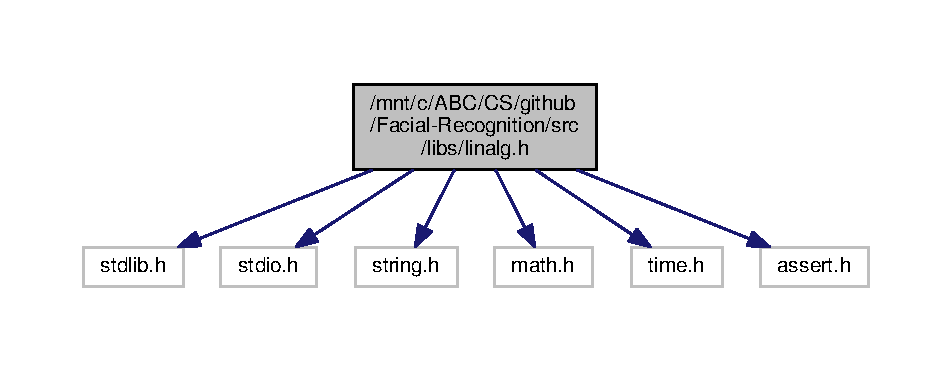
\includegraphics[width=350pt]{linalg_8h__incl}
\end{center}
\end{figure}
This graph shows which files directly or indirectly include this file\-:
\nopagebreak
\begin{figure}[H]
\begin{center}
\leavevmode
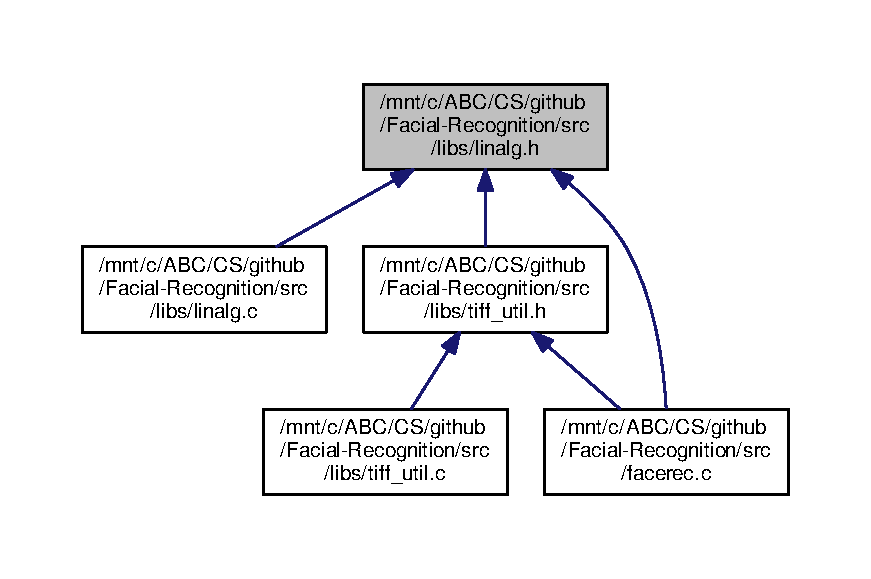
\includegraphics[width=350pt]{linalg_8h__dep__incl}
\end{center}
\end{figure}
\subsection*{Classes}
\begin{DoxyCompactItemize}
\item 
struct \hyperlink{struct__vector}{\-\_\-vector}
\begin{DoxyCompactList}\small\item\em represents a vector padding is to make sure that matrix and vector both have the same byte size and allignment between matrix and vector they are able to be casted into one another \end{DoxyCompactList}\item 
struct \hyperlink{struct__matrix}{\-\_\-matrix}
\begin{DoxyCompactList}\small\item\em represents a matrix between matrix and vector they are able to be casted into one another \end{DoxyCompactList}\end{DoxyCompactItemize}
\subsection*{Macros}
\begin{DoxyCompactItemize}
\item 
\hypertarget{linalg_8h_ae0e32e641b8137c777d52988864296e3}{\#define \hyperlink{linalg_8h_ae0e32e641b8137c777d52988864296e3}{M\-A\-T}(m, x, y)~(m-\/$>$data\mbox{[}(x $\ast$ m-\/$>$col) + y\mbox{]})}\label{linalg_8h_ae0e32e641b8137c777d52988864296e3}

\begin{DoxyCompactList}\small\item\em macro for element access in a matrix struct \end{DoxyCompactList}\item 
\hypertarget{linalg_8h_a03e904294c904b01194a25323fc2f6ec}{\#define \hyperlink{linalg_8h_a03e904294c904b01194a25323fc2f6ec}{V\-E\-C}(v, x)~(v-\/$>$data\mbox{[}x\mbox{]})}\label{linalg_8h_a03e904294c904b01194a25323fc2f6ec}

\begin{DoxyCompactList}\small\item\em macro for element access in a vector struct \end{DoxyCompactList}\end{DoxyCompactItemize}
\subsection*{Typedefs}
\begin{DoxyCompactItemize}
\item 
\hypertarget{linalg_8h_a07a01529159cc35e78c1f7731ac7bda6}{typedef struct \hyperlink{struct__vector}{\-\_\-vector} \hyperlink{linalg_8h_a07a01529159cc35e78c1f7731ac7bda6}{vector}}\label{linalg_8h_a07a01529159cc35e78c1f7731ac7bda6}

\begin{DoxyCompactList}\small\item\em represents a vector padding is to make sure that matrix and vector both have the same byte size and allignment between matrix and vector they are able to be casted into one another \end{DoxyCompactList}\item 
\hypertarget{linalg_8h_abc75382643898dd572498a574bf891c7}{typedef struct \hyperlink{struct__matrix}{\-\_\-matrix} \hyperlink{linalg_8h_abc75382643898dd572498a574bf891c7}{matrix}}\label{linalg_8h_abc75382643898dd572498a574bf891c7}

\begin{DoxyCompactList}\small\item\em represents a matrix between matrix and vector they are able to be casted into one another \end{DoxyCompactList}\end{DoxyCompactItemize}
\subsection*{Functions}
\begin{DoxyCompactItemize}
\item 
\hyperlink{linalg_8h_a07a01529159cc35e78c1f7731ac7bda6}{vector} $\ast$ \hyperlink{linalg_8h_a7040be230e99648e77b0932600bf55ef}{vector\-\_\-create} (size\-\_\-t size)
\begin{DoxyCompactList}\small\item\em Creates a vector this function will malloc the exact space for the required dimensions. \end{DoxyCompactList}\item 
\hyperlink{linalg_8h_abc75382643898dd572498a574bf891c7}{matrix} $\ast$ \hyperlink{linalg_8h_a7821976cc30bc3131f3646bec1992d91}{matrix\-\_\-create} (size\-\_\-t row, size\-\_\-t col)
\begin{DoxyCompactList}\small\item\em Creates a matrix this function will malloc the exact space for the required dimensions. \end{DoxyCompactList}\item 
\hyperlink{linalg_8h_abc75382643898dd572498a574bf891c7}{matrix} $\ast$ \hyperlink{linalg_8h_a8a5d3412faa2267345b3a7d1ca6f58c1}{vec\-\_\-to\-\_\-mat} (\hyperlink{linalg_8h_a07a01529159cc35e78c1f7731ac7bda6}{vector} $\ast$vec, int orientation)
\begin{DoxyCompactList}\small\item\em Converts vector into matrix this function will \char`\"{}cast\char`\"{} the vector into a matrix by using the fact that they both have the same size. when calling this function, calling free() on the matrix will free the vector and vice versa. \end{DoxyCompactList}\item 
\hyperlink{linalg_8h_a07a01529159cc35e78c1f7731ac7bda6}{vector} $\ast$ \hyperlink{linalg_8h_a9059a420799b3aa9c04d5dd469523d91}{mat\-\_\-to\-\_\-vec} (\hyperlink{linalg_8h_abc75382643898dd572498a574bf891c7}{matrix} $\ast$mat)
\begin{DoxyCompactList}\small\item\em Converts matrix into vector this function will \char`\"{}cast\char`\"{} the matrix into a vector by using the fact that they both have the same size. when calling this function, calling free() on the vector will free the matrix and vice versa. the input matrix can only be a matrix with dimensions 1 X N (a row matrix) \end{DoxyCompactList}\item 
void \hyperlink{linalg_8h_a41ab46fdaa678c67aef38d873870a98d}{matrix\-\_\-reshape} (\hyperlink{linalg_8h_abc75382643898dd572498a574bf891c7}{matrix} $\ast$mat, size\-\_\-t row, size\-\_\-t col)
\begin{DoxyCompactList}\small\item\em Reshapes the matrix this function will reshape the matrix in constant time. \end{DoxyCompactList}\item 
double \hyperlink{linalg_8h_afc298e7d7d6a208e71ef073948b651d2}{dot\-\_\-product} (const double $\ast$left, const double $\ast$right, int length)
\begin{DoxyCompactList}\small\item\em Performs dot product on two double$\ast$ this function will malloc for the user a double arrays must be of same size. \end{DoxyCompactList}\item 
\hyperlink{linalg_8h_a07a01529159cc35e78c1f7731ac7bda6}{vector} $\ast$ \hyperlink{linalg_8h_a0c350b8673e50738602aa10cd6a86924}{vecscalar\-\_\-multiply} (const \hyperlink{linalg_8h_a07a01529159cc35e78c1f7731ac7bda6}{vector} $\ast$vec, const double scalar)
\begin{DoxyCompactList}\small\item\em Performs scalar multiplication of a vector this function will malloc for the user a vector$\ast$. \end{DoxyCompactList}\item 
\hyperlink{linalg_8h_a07a01529159cc35e78c1f7731ac7bda6}{vector} $\ast$ \hyperlink{linalg_8h_a2bc6dcc923c28a9d6f0ff38bd5de55f5}{vecscalar\-\_\-divide} (const \hyperlink{linalg_8h_a07a01529159cc35e78c1f7731ac7bda6}{vector} $\ast$vec, const double scalar)
\begin{DoxyCompactList}\small\item\em Performs scalar division of a vector this function will malloc for the user a vector$\ast$. \end{DoxyCompactList}\item 
\hyperlink{linalg_8h_a07a01529159cc35e78c1f7731ac7bda6}{vector} $\ast$ \hyperlink{linalg_8h_a4af2cd71186eeb14f970f97a27fbcef0}{vecmat\-\_\-multiply} (const \hyperlink{linalg_8h_a07a01529159cc35e78c1f7731ac7bda6}{vector} $\ast$vec, const \hyperlink{linalg_8h_abc75382643898dd572498a574bf891c7}{matrix} $\ast$mat)
\begin{DoxyCompactList}\small\item\em Performs vector matrix multiplication this function will malloc for the user a vector$\ast$ if the vector is of size M and the matrix size M by N, the resulting column vector will be of size N. \end{DoxyCompactList}\item 
\hyperlink{linalg_8h_a07a01529159cc35e78c1f7731ac7bda6}{vector} $\ast$ \hyperlink{linalg_8h_af88415d8996030537851e2c48d5337c4}{matvec\-\_\-multiply} (const \hyperlink{linalg_8h_abc75382643898dd572498a574bf891c7}{matrix} $\ast$mat, const \hyperlink{linalg_8h_a07a01529159cc35e78c1f7731ac7bda6}{vector} $\ast$vec)
\begin{DoxyCompactList}\small\item\em Performs matrix vector multiplication this function will malloc for the user a vector$\ast$ if the matrix is of size M by N and the vector N, the resulting row vector will be of size M. \end{DoxyCompactList}\item 
void \hyperlink{linalg_8h_a3c4e05af95e01c11963c912837d0d35b}{mat\-\_\-print} (const \hyperlink{linalg_8h_abc75382643898dd572498a574bf891c7}{matrix} $\ast$mat)
\begin{DoxyCompactList}\small\item\em prints the matrix this function will not modify the matrix and print to stdout \end{DoxyCompactList}\item 
void \hyperlink{linalg_8h_a1d2e72678bf82c44ba57020fc8588868}{vec\-\_\-print} (const \hyperlink{linalg_8h_a07a01529159cc35e78c1f7731ac7bda6}{vector} $\ast$vec)
\begin{DoxyCompactList}\small\item\em prints the vector this function will not modify the vector and print to stdout \end{DoxyCompactList}\item 
\hyperlink{linalg_8h_abc75382643898dd572498a574bf891c7}{matrix} $\ast$ \hyperlink{linalg_8h_a40a3d6442169157a458362f5e85c5843}{matmat\-\_\-multiply} (const \hyperlink{linalg_8h_abc75382643898dd572498a574bf891c7}{matrix} $\ast$left, const \hyperlink{linalg_8h_abc75382643898dd572498a574bf891c7}{matrix} $\ast$right)
\begin{DoxyCompactList}\small\item\em Performs standard matrix multiplication this function will malloc for the user a matrix$\ast$. \end{DoxyCompactList}\item 
\hyperlink{linalg_8h_abc75382643898dd572498a574bf891c7}{matrix} $\ast$ \hyperlink{linalg_8h_a9d1ca6441796b3d9c53f2a2923dc06c7}{matmat\-\_\-addition} (const \hyperlink{linalg_8h_abc75382643898dd572498a574bf891c7}{matrix} $\ast$left, const \hyperlink{linalg_8h_abc75382643898dd572498a574bf891c7}{matrix} $\ast$right)
\begin{DoxyCompactList}\small\item\em Performs standard matrix addition this function will malloc for the user a matrix$\ast$. \end{DoxyCompactList}\item 
\hyperlink{linalg_8h_abc75382643898dd572498a574bf891c7}{matrix} $\ast$ \hyperlink{linalg_8h_a6b7138d5fae752feceeb9faea996cb54}{matmat\-\_\-subtraction} (const \hyperlink{linalg_8h_abc75382643898dd572498a574bf891c7}{matrix} $\ast$left, const \hyperlink{linalg_8h_abc75382643898dd572498a574bf891c7}{matrix} $\ast$right)
\begin{DoxyCompactList}\small\item\em Performs standard matrix subtration this function will malloc for the user a matrix$\ast$. \end{DoxyCompactList}\item 
\hyperlink{linalg_8h_abc75382643898dd572498a574bf891c7}{matrix} $\ast$ \hyperlink{linalg_8h_a32cb81b161008e2b1fd862ae9d45caa2}{matscalar\-\_\-multiply} (const \hyperlink{linalg_8h_abc75382643898dd572498a574bf891c7}{matrix} $\ast$mat, const double scalar)
\begin{DoxyCompactList}\small\item\em Performs scalar multiplication of a matrix this function will malloc for the user a matrix$\ast$. \end{DoxyCompactList}\item 
\hyperlink{linalg_8h_abc75382643898dd572498a574bf891c7}{matrix} $\ast$ \hyperlink{linalg_8h_a98269f4c3f77b32dc52e30108713cb28}{matscalar\-\_\-divide} (const \hyperlink{linalg_8h_abc75382643898dd572498a574bf891c7}{matrix} $\ast$mat, const double scalar)
\begin{DoxyCompactList}\small\item\em Performs scalar division of a matrix this function will malloc for the user a matrix$\ast$. \end{DoxyCompactList}\item 
\hyperlink{linalg_8h_abc75382643898dd572498a574bf891c7}{matrix} $\ast$ \hyperlink{linalg_8h_a2ac4400497d3a421f3f631d6329010b6}{mat\-\_\-transpose} (const \hyperlink{linalg_8h_abc75382643898dd572498a574bf891c7}{matrix} $\ast$mat)
\begin{DoxyCompactList}\small\item\em Performs matrix transpose this function will malloc for the user a matrix$\ast$. \end{DoxyCompactList}\item 
void \hyperlink{linalg_8h_adbfad21fe7e851455d625173e67b8504}{vec\-\_\-append} (\hyperlink{linalg_8h_a07a01529159cc35e78c1f7731ac7bda6}{vector} $\ast$$\ast$vec\-\_\-a, \hyperlink{linalg_8h_a07a01529159cc35e78c1f7731ac7bda6}{vector} $\ast$vec\-\_\-b)
\begin{DoxyCompactList}\small\item\em Appends vector b to vector a this function will realloc for the user vector a and free vector b. \end{DoxyCompactList}\item 
void \hyperlink{linalg_8h_a2488d3254a915ffec423a4355b6a32a3}{eigen} (int N, double a\mbox{[}$\,$\mbox{]}, int it\-\_\-max, double v\mbox{[}$\,$\mbox{]}, double d\mbox{[}$\,$\mbox{]}, int $\ast$it\-\_\-num, int $\ast$rot\-\_\-num)
\begin{DoxyCompactList}\small\item\em Performs Jacobi eigenvalue iteration this function will required the user to pass in non-\/null it\-\_\-num and rot\-\_\-num it does not malloc but rather requires the caller to malloc space for it. \end{DoxyCompactList}\item 
void \hyperlink{linalg_8h_a97f97bfa6f100928e8d6c9f085bd9d12}{mat\-\_\-identity} (int n, double a\mbox{[}$\,$\mbox{]})
\begin{DoxyCompactList}\small\item\em modifies a matrix to be the identity matrix of size n \end{DoxyCompactList}\item 
void \hyperlink{linalg_8h_abc4918a0c6b295404ebfadfe78b26bdd}{diag\-\_\-vector} (int n, double a\mbox{[}$\,$\mbox{]}, double v\mbox{[}$\,$\mbox{]})
\begin{DoxyCompactList}\small\item\em gets the diagonal entries \end{DoxyCompactList}\item 
double \hyperlink{linalg_8h_a948f2b3da29647be0bcb62e717dfec2d}{frobenius\-\_\-norm} (int n, int k, double a\mbox{[}$\,$\mbox{]}, double x\mbox{[}$\,$\mbox{]}, double lambda\mbox{[}$\,$\mbox{]})
\begin{DoxyCompactList}\small\item\em computes the Frobenius norm in a right eigensystem \end{DoxyCompactList}\item 
\hyperlink{linalg_8h_abc75382643898dd572498a574bf891c7}{matrix} $\ast$ \hyperlink{linalg_8h_ad41ec0281d3766f40963b77520ce600d}{covmat} (\hyperlink{linalg_8h_abc75382643898dd572498a574bf891c7}{matrix} $\ast$mat)
\begin{DoxyCompactList}\small\item\em computes the variance covariance matrix \end{DoxyCompactList}\item 
\hyperlink{linalg_8h_a07a01529159cc35e78c1f7731ac7bda6}{vector} $\ast$ \hyperlink{linalg_8h_a71f490da601d057f4ce45efb9a48c2ae}{compute\-\_\-average} (\hyperlink{linalg_8h_abc75382643898dd572498a574bf891c7}{matrix} $\ast$images, int num\-\_\-images)
\begin{DoxyCompactList}\small\item\em computes the average matrix of all the $\ast$vector images \end{DoxyCompactList}\end{DoxyCompactItemize}


\subsection{Detailed Description}
File containing common linear algebra functions. Minhyuk Park \begin{DoxyDate}{Date}
7 Nov 2017 
\end{DoxyDate}


\subsection{Function Documentation}
\hypertarget{linalg_8h_a71f490da601d057f4ce45efb9a48c2ae}{\index{linalg.\-h@{linalg.\-h}!compute\-\_\-average@{compute\-\_\-average}}
\index{compute\-\_\-average@{compute\-\_\-average}!linalg.h@{linalg.\-h}}
\subsubsection[{compute\-\_\-average}]{\setlength{\rightskip}{0pt plus 5cm}{\bf vector}$\ast$ compute\-\_\-average (
\begin{DoxyParamCaption}
\item[{{\bf matrix} $\ast$}]{images, }
\item[{int}]{num\-\_\-images}
\end{DoxyParamCaption}
)}}\label{linalg_8h_a71f490da601d057f4ce45efb9a48c2ae}


computes the average matrix of all the $\ast$vector images 

\begin{DoxyReturn}{Returns}
vector$\ast$ the average image 
\end{DoxyReturn}

\begin{DoxyParams}{Parameters}
{\em images} & matrix$\ast$ a matrix where each column represents an image \\
\hline
{\em num\-\_\-images} & int number of images in the vector \\
\hline
\end{DoxyParams}


References M\-A\-T, \-\_\-matrix\-::row, \-\_\-vector\-::size, V\-E\-C, and vector\-\_\-create().


\begin{DoxyCode}
407                                                         \{
408     \textcolor{comment}{/*}
409 \textcolor{comment}{    matrix* ones\_row = matrix\_create(1, num\_images);
}
410 \textcolor{comment}{    for(int i =0; i <num\_images; i++) \{
}
411 \textcolor{comment}{        MAT(ones\_row, 0,i) = 1;
}
412 \textcolor{comment}{    \}
}
413 \textcolor{comment}{    matrix* row\_images = mat\_transpose(images);
}
414 \textcolor{comment}{    matrix* row\_sum = matmat\_multiply(ones\_row, row\_images);
}
415 \textcolor{comment}{    vector* vector\_row\_sum = mat\_to\_vec(row\_sum);
}
416 \textcolor{comment}{    vector* img\_avg = vecscalar\_divide(vector\_row\_sum, num\_images);
}
417 \textcolor{comment}{    free(vector\_row\_sum);
}
418 \textcolor{comment}{    free(row\_images);
}
419 \textcolor{comment}{    free(ones\_row);
}
420 \textcolor{comment}{    */}
421     \hyperlink{struct__vector}{vector}* img\_avg = \hyperlink{linalg_8c_a7040be230e99648e77b0932600bf55ef}{vector\_create}(images->\hyperlink{struct__matrix_a1087bec6a11b0773b4852c4ca49fc32a}{row});
422 
423     \textcolor{keywordflow}{for}(\textcolor{keywordtype}{size\_t} i = 0; i < img\_avg->\hyperlink{struct__vector_a1ed8dca78f3e589deb8dad9b53aec3fa}{size}; i ++) \{
424         uint32 avg\_pixel = 0;
425 
426         uint32 r = 0;
427         uint32 g = 0;
428         uint32 b = 0;
429         uint32 a = 0;
430         \textcolor{keywordflow}{for}(\textcolor{keywordtype}{int} j = 0; j < num\_images; j ++) \{
431             uint32 current\_pixel = \hyperlink{linalg_8h_ae0e32e641b8137c777d52988864296e3}{MAT}(images, i, j);
432 
433             r += ((current\_pixel & 0xff) * (current\_pixel & 0xff));
434             g += (((current\_pixel >> 8) & 0xff) * ((current\_pixel >> 8) & 0xff));
435             b += (((current\_pixel >> 16) & 0xff) * ((current\_pixel >> 16) & 0xff));
436             a += (((current\_pixel >> 24) & 0xff) * ((current\_pixel >> 24) & 0xff));
437         \}
438 
439         r /= num\_images;
440         g /= num\_images;
441         b /= num\_images;
442         a /= num\_images;
443 
444         r = sqrt(r);
445         g = sqrt(g);
446         b = sqrt(b);
447         a = sqrt(a);
448         \textcolor{comment}{/*}
449 \textcolor{comment}{        for(int j = 0; j < num\_images; j ++) \{
}
450 \textcolor{comment}{            uint32 current\_pixel = MAT(images, i, j);
}
451 \textcolor{comment}{}
452 \textcolor{comment}{            r += ((current\_pixel & 0xff));
}
453 \textcolor{comment}{            g += (((current\_pixel >> 8) & 0xff));
}
454 \textcolor{comment}{            b += (((current\_pixel >> 16) & 0xff));
}
455 \textcolor{comment}{            a += (((current\_pixel >> 24) & 0xff));
}
456 \textcolor{comment}{        \}
}
457 \textcolor{comment}{}
458 \textcolor{comment}{        r /= num\_images;
}
459 \textcolor{comment}{        g /= num\_images;
}
460 \textcolor{comment}{        b /= num\_images;
}
461 \textcolor{comment}{        a /= num\_images;
}
462 \textcolor{comment}{        */}
463 
464 
465         avg\_pixel |= r;
466         avg\_pixel |= (g << 8);
467         avg\_pixel |= (b << 16);
468         avg\_pixel |= (a << 24);
469 
470         \hyperlink{linalg_8h_a03e904294c904b01194a25323fc2f6ec}{VEC}(img\_avg, i) = avg\_pixel;
471     \}
472 
473 
474     
475 
476     \textcolor{keywordflow}{return} img\_avg;
477 \}
\end{DoxyCode}
\hypertarget{linalg_8h_ad41ec0281d3766f40963b77520ce600d}{\index{linalg.\-h@{linalg.\-h}!covmat@{covmat}}
\index{covmat@{covmat}!linalg.h@{linalg.\-h}}
\subsubsection[{covmat}]{\setlength{\rightskip}{0pt plus 5cm}{\bf matrix}$\ast$ covmat (
\begin{DoxyParamCaption}
\item[{{\bf matrix} $\ast$}]{mat}
\end{DoxyParamCaption}
)}}\label{linalg_8h_ad41ec0281d3766f40963b77520ce600d}


computes the variance covariance matrix 

\begin{DoxyReturn}{Returns}
matrix$\ast$ the output variance-\/covariance matrix this function will malloc a new matrix 
\end{DoxyReturn}

\begin{DoxyParams}{Parameters}
{\em mat} & a matrix$\ast$ representing the input matrix of deviation scores of size n by k \\
\hline
\end{DoxyParams}


References mat\-\_\-transpose(), matmat\-\_\-multiply(), matscalar\-\_\-divide(), and \-\_\-matrix\-::row.


\begin{DoxyCode}
397                             \{
398     \textcolor{keywordtype}{size\_t} n = mat->\hyperlink{struct__matrix_a1087bec6a11b0773b4852c4ca49fc32a}{row};
399     \hyperlink{struct__matrix}{matrix}* mat\_T = \hyperlink{linalg_8c_a2ac4400497d3a421f3f631d6329010b6}{mat\_transpose}(mat);
400     \hyperlink{struct__matrix}{matrix}* x\_T\_x = \hyperlink{linalg_8c_a40a3d6442169157a458362f5e85c5843}{matmat\_multiply}(mat\_T, mat);
401     \hyperlink{struct__matrix}{matrix}* retmat = \hyperlink{linalg_8c_a98269f4c3f77b32dc52e30108713cb28}{matscalar\_divide}(x\_T\_x, n);
402     free(x\_T\_x);
403     free(mat\_T);
404     \textcolor{keywordflow}{return} retmat;
405 \}
\end{DoxyCode}
\hypertarget{linalg_8h_abc4918a0c6b295404ebfadfe78b26bdd}{\index{linalg.\-h@{linalg.\-h}!diag\-\_\-vector@{diag\-\_\-vector}}
\index{diag\-\_\-vector@{diag\-\_\-vector}!linalg.h@{linalg.\-h}}
\subsubsection[{diag\-\_\-vector}]{\setlength{\rightskip}{0pt plus 5cm}void diag\-\_\-vector (
\begin{DoxyParamCaption}
\item[{int}]{n, }
\item[{double}]{a\mbox{[}$\,$\mbox{]}, }
\item[{double}]{v\mbox{[}$\,$\mbox{]}}
\end{DoxyParamCaption}
)}}\label{linalg_8h_abc4918a0c6b295404ebfadfe78b26bdd}


gets the diagonal entries 


\begin{DoxyParams}{Parameters}
{\em n} & int the dimension \\
\hline
{\em a\mbox{[}$\,$\mbox{]}} & double\mbox{[}\mbox{]} input the matrix, N by N \\
\hline
{\em v\mbox{[}$\,$\mbox{]}} & double\mbox{[}\mbox{]} output the diagonal entries, N \\
\hline
\end{DoxyParams}


Referenced by eigen().


\begin{DoxyCode}
363                                                 \{
364     \textcolor{keywordflow}{for}(\textcolor{keywordtype}{int} i = 0; i < n; i ++) \{
365         v[i] = a[i + i * n];
366     \}
367     \textcolor{keywordflow}{return};
368 \}
\end{DoxyCode}
\hypertarget{linalg_8h_afc298e7d7d6a208e71ef073948b651d2}{\index{linalg.\-h@{linalg.\-h}!dot\-\_\-product@{dot\-\_\-product}}
\index{dot\-\_\-product@{dot\-\_\-product}!linalg.h@{linalg.\-h}}
\subsubsection[{dot\-\_\-product}]{\setlength{\rightskip}{0pt plus 5cm}double dot\-\_\-product (
\begin{DoxyParamCaption}
\item[{const double $\ast$}]{left, }
\item[{const double $\ast$}]{right, }
\item[{int}]{length}
\end{DoxyParamCaption}
)}}\label{linalg_8h_afc298e7d7d6a208e71ef073948b651d2}


Performs dot product on two double$\ast$ this function will malloc for the user a double arrays must be of same size. 

\begin{DoxyReturn}{Returns}
a double representing the inner product 
\end{DoxyReturn}

\begin{DoxyParams}{Parameters}
{\em left} & const double$\ast$ the first vector \\
\hline
{\em right} & const double$\ast$ the second vector \\
\hline
{\em length} & int the size of the vectors \\
\hline
\end{DoxyParams}


Referenced by matvec\-\_\-multiply().


\begin{DoxyCode}
57                                                                         \{
58     \textcolor{keywordtype}{double} retval = 0.0;
59     \textcolor{keywordflow}{for}(\textcolor{keywordtype}{int} i = 0; i < length; i ++) \{
60         retval += (left[i] * right[i]);
61     \}
62     \textcolor{keywordflow}{return} retval;
63 \}
\end{DoxyCode}
\hypertarget{linalg_8h_a2488d3254a915ffec423a4355b6a32a3}{\index{linalg.\-h@{linalg.\-h}!eigen@{eigen}}
\index{eigen@{eigen}!linalg.h@{linalg.\-h}}
\subsubsection[{eigen}]{\setlength{\rightskip}{0pt plus 5cm}void eigen (
\begin{DoxyParamCaption}
\item[{int}]{N, }
\item[{double}]{a\mbox{[}$\,$\mbox{]}, }
\item[{int}]{it\-\_\-max, }
\item[{double}]{v\mbox{[}$\,$\mbox{]}, }
\item[{double}]{d\mbox{[}$\,$\mbox{]}, }
\item[{int $\ast$}]{it\-\_\-num, }
\item[{int $\ast$}]{rot\-\_\-num}
\end{DoxyParamCaption}
)}}\label{linalg_8h_a2488d3254a915ffec423a4355b6a32a3}


Performs Jacobi eigenvalue iteration this function will required the user to pass in non-\/null it\-\_\-num and rot\-\_\-num it does not malloc but rather requires the caller to malloc space for it. 


\begin{DoxyParams}{Parameters}
{\em N} & int the dimiension of the input matrix a, which is a N by N matrix \\
\hline
{\em a\mbox{[}$\,$\mbox{]}} & double\mbox{[}\mbox{]} the input matrix which has to be square, real, and symmetric \\
\hline
{\em it\-\_\-max} & int maximum number of iterations to stop at \\
\hline
{\em v\mbox{[}$\,$\mbox{]}} & double\mbox{[}\mbox{]}output matrix of eigenvectors, which is a N by N matrix \\
\hline
{\em d\mbox{[}$\,$\mbox{]}} & double\mbox{[}\mbox{]} output matrix of eigenvalues, in descending order \\
\hline
{\em it\-\_\-num} & int$\ast$ output total number of iterations \\
\hline
{\em rot\-\_\-num} & int$\ast$ output total number of rotations \\
\hline
\end{DoxyParams}


References diag\-\_\-vector(), and mat\-\_\-identity().


\begin{DoxyCode}
212                                                                                              \{
213     \hyperlink{linalg_8c_a97f97bfa6f100928e8d6c9f085bd9d12}{mat\_identity}(n, v); \textcolor{comment}{// create the identity matrix using what the caller allocated for us}
214     \hyperlink{linalg_8c_abc4918a0c6b295404ebfadfe78b26bdd}{diag\_vector}(n, a, d); \textcolor{comment}{// get the diagonal values of a and store it in caller allocated
       vector d}
215 
216     \textcolor{keywordtype}{double}* bw = (\textcolor{keywordtype}{double}*) malloc(n * \textcolor{keyword}{sizeof}(\textcolor{keywordtype}{double}));
217     \textcolor{keywordtype}{double}* zw = (\textcolor{keywordtype}{double}*) malloc(n * \textcolor{keyword}{sizeof}(\textcolor{keywordtype}{double}));
218 
219     \textcolor{keywordflow}{for}(\textcolor{keywordtype}{int} i = 0; i < n; i ++) \{
220         bw[i] = d[i];
221         zw[i] = 0.0;
222     \}
223     *it\_num = 0;
224     *rot\_num = 0;
225 
226     \textcolor{keywordtype}{double} thresh = 0.0;
227     \textcolor{keywordtype}{double} gapq = 0.0;
228     \textcolor{keywordflow}{while}(*it\_num < it\_max) \{
229         *it\_num += 1;
230         thresh = 0.0;
231         \textcolor{comment}{// set up the convergence threshold}
232         \textcolor{comment}{// based on the size of strict upper triangle}
233         \textcolor{keywordflow}{for}(\textcolor{keywordtype}{int} i = 0; i < n; i ++) \{
234             \textcolor{keywordflow}{for}(\textcolor{keywordtype}{int} j = 0; j < i; j ++) \{
235                 thresh += (a[j + i * n] * a[j + i * n]);
236             \}
237         \}
238         \textcolor{comment}{// PASS 1}
239         thresh = sqrt(thresh) / (double)(4 * n);
240         \textcolor{keywordflow}{if}(thresh == 0.0) \{
241             \textcolor{keywordflow}{break};
242         \}
243         \textcolor{comment}{// PASS 2}
244         \textcolor{keywordflow}{for}(\textcolor{keywordtype}{int} p = 0; p < n; p ++) \{
245             \textcolor{keywordflow}{for}(\textcolor{keywordtype}{int} q = p + 1; q < n; q ++) \{
246                 gapq = 10.0 * fabs(a[p + q * n]);
247                 \textcolor{keywordtype}{double} termp = gapq + fabs(d[p]);
248                 \textcolor{keywordtype}{double} termq = gapq + fabs(d[q]);
249                 \textcolor{keywordflow}{if}(4 < *it\_num && termp == fabs(d[p]) && termq == fabs(d[q])) \{
250                     a[p + q * n] = 0.0;
251                 \textcolor{comment}{// apply rotation otherwise}
252                 \textcolor{comment}{// PASS 3}
253                 \} \textcolor{keywordflow}{else} \textcolor{keywordflow}{if}(thresh <= fabs(a[p + q * n])) \{
254                     \textcolor{keywordtype}{double} h = d[q] - d[p];
255                     \textcolor{keywordtype}{double} term = fabs(h) + gapq;
256                     \textcolor{keywordtype}{double} t = 0.0;
257                     \textcolor{keywordflow}{if}(term == fabs(h)) \{
258                         t = a[p + q * n] / h;
259                     \} \textcolor{keywordflow}{else} \{
260                         \textcolor{keywordtype}{double} theta = 0.5 * h / a[p + q * n];
261                         t = 1.0 / (fabs(theta) + sqrt(1.0 + theta * theta));
262                         \textcolor{keywordflow}{if}(theta < 0.0) \{
263                             t = -t;
264                         \}
265                     \}
266                     \textcolor{comment}{// PASS 4}
267                     \textcolor{keywordtype}{double} c = 1.0 / sqrt(1.0 + t * t);
268                     \textcolor{keywordtype}{double} s = t * c;
269                     \textcolor{keywordtype}{double} tau = s / (1.0 + c);
270                     h = t * a[p + q * n];
271 
272                     zw[p] -= h;
273                     zw[q] += h;
274                     d[p] -= h;
275                     d[q] += h;
276                     a[p + q * n] = 0.0;
277                     \textcolor{comment}{// PASS 5}
278                     \textcolor{comment}{// rotate}
279                     \textcolor{keywordtype}{double} g = 0.0;
280                     \textcolor{keywordflow}{for}(\textcolor{keywordtype}{int} j = 0; j < p; j ++) \{
281                         g = a[j + p * n];
282                         h = a[j + q * n];
283                         a[j + p * n] = g - s * (h + g * tau);
284                         a[j + q * n] = h + s * (g - h * tau);
285                     \}
286                     \textcolor{keywordflow}{for}(\textcolor{keywordtype}{int} j = p + 1; j < q; j ++) \{
287                         g = a[p + j * n];
288                         h = a[j + q * n];
289                         a[p + j * n] = g - s * (h + g * tau);
290                         a[j + q * n] = h + s * (g - h * tau);
291                     \}
292                     \textcolor{keywordflow}{for}(\textcolor{keywordtype}{int} j = q + 1; j < n; j ++) \{
293                         g = a[p + j * n];
294                         h = a[q + j * n];
295                         a[p + j * n] = g - s * (h + g * tau);
296                         a[q + j * n] = h + s * (g - h * tau);
297                     \}
298                     \textcolor{comment}{// PASS 6}
299                     \textcolor{comment}{// store to eigenvector matrix v}
300                     \textcolor{keywordflow}{for}(\textcolor{keywordtype}{int} j = 0; j < n; j ++) \{
301                         g = v[j + p * n];
302                         h = v[j + q * n];
303                         v[j + p * n] = g - s * (h + g * tau);
304                         v[j + q * n] = h + s * (g - h * tau);
305                     \}
306                     *rot\_num += 1;
307                 \}
308             \}
309         \}
310         \textcolor{keywordflow}{for}(\textcolor{keywordtype}{int} i = 0; i < n; i ++) \{
311             bw[i] += zw[i];
312             d[i] = bw[i];
313             zw[i] = 0.0;
314         \}
315     \}
316     \textcolor{comment}{// PASS 7}
317     \textcolor{comment}{// restore upper triangle}
318     \textcolor{keywordflow}{for}(\textcolor{keywordtype}{int} i = 0; i < n; i ++) \{
319         \textcolor{keywordflow}{for}(\textcolor{keywordtype}{int} j = 0; j < i; j ++) \{
320             a[j + i * n] = a [i + j * n];
321         \}
322     \}
323     \textcolor{keywordflow}{for}(\textcolor{keywordtype}{int} k = 0; k < n - 1; k ++) \{
324         \textcolor{keywordtype}{int} m = k;
325         \textcolor{keywordflow}{for}(\textcolor{keywordtype}{int} l = k + 1; l < n; l ++) \{
326             \textcolor{keywordflow}{if}(d[l] < d[m]) \{
327                 m = l;
328             \}
329         \}
330         \textcolor{keywordflow}{if}(m != k) \{
331             \textcolor{keywordtype}{double} t = d[m];
332             d[m] = d[k];
333             d[k] = t;
334             \textcolor{keywordflow}{for}(\textcolor{keywordtype}{int} i = 0; i < n; i ++) \{
335                 \textcolor{keywordtype}{double} w = v[i + m * n];
336                 v[i + m * n] = v[i + k * n];
337                 v[i + k * n] = w;
338             \}
339         \}
340     \}
341     free(bw);
342     free(zw);
343     \textcolor{keywordflow}{return};
344 \}
\end{DoxyCode}
\hypertarget{linalg_8h_a948f2b3da29647be0bcb62e717dfec2d}{\index{linalg.\-h@{linalg.\-h}!frobenius\-\_\-norm@{frobenius\-\_\-norm}}
\index{frobenius\-\_\-norm@{frobenius\-\_\-norm}!linalg.h@{linalg.\-h}}
\subsubsection[{frobenius\-\_\-norm}]{\setlength{\rightskip}{0pt plus 5cm}double frobenius\-\_\-norm (
\begin{DoxyParamCaption}
\item[{int}]{n, }
\item[{int}]{k, }
\item[{double}]{a\mbox{[}$\,$\mbox{]}, }
\item[{double}]{x\mbox{[}$\,$\mbox{]}, }
\item[{double}]{lambda\mbox{[}$\,$\mbox{]}}
\end{DoxyParamCaption}
)}}\label{linalg_8h_a948f2b3da29647be0bcb62e717dfec2d}


computes the Frobenius norm in a right eigensystem 

\begin{DoxyReturn}{Returns}
double the frobenius norm of A $\ast$ X -\/ X $\ast$ lambda 
\end{DoxyReturn}

\begin{DoxyParams}{Parameters}
{\em n} & int the dimension of the matrix \\
\hline
{\em k} & int the number of eigen vectors \\
\hline
{\em a\mbox{[}$\,$\mbox{]}} & double\mbox{[}\mbox{]} input matrix of size n by n \\
\hline
{\em x\mbox{[}$\,$\mbox{]}} & double\mbox{[}\mbox{]} input vector of eigenvectors of size k \\
\hline
{\em lamdba\mbox{[}$\,$\mbox{]}} & double\mbox{[}\mbox{]} input vector of eigen values \\
\hline
\end{DoxyParams}

\begin{DoxyCode}
371                                                                              \{
372     \textcolor{keywordtype}{double}* c = (\textcolor{keywordtype}{double}*) malloc(n * k * \textcolor{keyword}{sizeof}(\textcolor{keywordtype}{double}));
373     \textcolor{keywordflow}{for}(\textcolor{keywordtype}{int} i = 0; i < k; i ++) \{
374         \textcolor{keywordflow}{for}(\textcolor{keywordtype}{int} j = 0; j < n; j ++) \{
375             c[j + i * n] = 0.0;
376             \textcolor{keywordflow}{for}(\textcolor{keywordtype}{int} l = 0; l < n; l ++) \{
377                 c[j + i * n] = c[j + i * n] + a[j + l * n] * x[l + i * n];
378             \}
379         \}
380     \}
381     \textcolor{keywordflow}{for}(\textcolor{keywordtype}{int} i = 0; i < k; i ++) \{
382         \textcolor{keywordflow}{for}(\textcolor{keywordtype}{int} j = 0; j < n; j ++) \{
383             c[j + i * n] = c[j + i * n] - lambda[i] * x[j + i * n];
384         \}
385     \}
386     \textcolor{keywordtype}{double} retval = 0.0;
387     \textcolor{keywordflow}{for}(\textcolor{keywordtype}{int} i = 0; i < k; i ++) \{
388         \textcolor{keywordflow}{for}(\textcolor{keywordtype}{int} j = 0; j < n; j ++) \{
389             retval += pow(c[j + i * n], 2);
390         \}
391     \}
392     retval = sqrt(retval);
393     free(c);
394     \textcolor{keywordflow}{return} retval;
395 \}
\end{DoxyCode}
\hypertarget{linalg_8h_a97f97bfa6f100928e8d6c9f085bd9d12}{\index{linalg.\-h@{linalg.\-h}!mat\-\_\-identity@{mat\-\_\-identity}}
\index{mat\-\_\-identity@{mat\-\_\-identity}!linalg.h@{linalg.\-h}}
\subsubsection[{mat\-\_\-identity}]{\setlength{\rightskip}{0pt plus 5cm}void mat\-\_\-identity (
\begin{DoxyParamCaption}
\item[{int}]{n, }
\item[{double}]{a\mbox{[}$\,$\mbox{]}}
\end{DoxyParamCaption}
)}}\label{linalg_8h_a97f97bfa6f100928e8d6c9f085bd9d12}


modifies a matrix to be the identity matrix of size n 


\begin{DoxyParams}{Parameters}
{\em n} & int the dimension \\
\hline
{\em a\mbox{[}$\,$\mbox{]}} & double output identity matrix \\
\hline
\end{DoxyParams}


Referenced by eigen().


\begin{DoxyCode}
347                                      \{
348     \textcolor{keywordtype}{int} k = 0;
349     \textcolor{keywordflow}{for} (\textcolor{keywordtype}{int} j = 0; j < n; j ++ ) \{
350         \textcolor{keywordflow}{for} (\textcolor{keywordtype}{int} i = 0; i < n; i ++ ) \{
351             \textcolor{keywordflow}{if} ( i == j ) \{
352                 a[k] = 1.0;
353             \} \textcolor{keywordflow}{else} \{
354                 a[k] = 0.0;
355             \}
356             k += 1;
357         \}
358     \}
359     \textcolor{keywordflow}{return};
360 \}
\end{DoxyCode}
\hypertarget{linalg_8h_a3c4e05af95e01c11963c912837d0d35b}{\index{linalg.\-h@{linalg.\-h}!mat\-\_\-print@{mat\-\_\-print}}
\index{mat\-\_\-print@{mat\-\_\-print}!linalg.h@{linalg.\-h}}
\subsubsection[{mat\-\_\-print}]{\setlength{\rightskip}{0pt plus 5cm}void mat\-\_\-print (
\begin{DoxyParamCaption}
\item[{const {\bf matrix} $\ast$}]{mat}
\end{DoxyParamCaption}
)}}\label{linalg_8h_a3c4e05af95e01c11963c912837d0d35b}


prints the matrix this function will not modify the matrix and print to stdout 


\begin{DoxyParams}{Parameters}
{\em mat} & const matrix$\ast$ the matrix to be printed \\
\hline
\end{DoxyParams}


References \-\_\-matrix\-::col, M\-A\-T, and \-\_\-matrix\-::row.


\begin{DoxyCode}
107                                   \{
108     \textcolor{keywordflow}{for}(\textcolor{keywordtype}{size\_t} i = 0; i < mat->\hyperlink{struct__matrix_a1087bec6a11b0773b4852c4ca49fc32a}{row}; i ++) \{
109         \textcolor{keywordflow}{for}(\textcolor{keywordtype}{size\_t} j = 0; j < mat->\hyperlink{struct__matrix_a7e9feb52cfc0a9d7cba5320abcaa997a}{col}; j ++) \{
110             \textcolor{keywordflow}{if}(j == mat->\hyperlink{struct__matrix_a7e9feb52cfc0a9d7cba5320abcaa997a}{col} - 1) \{
111                 printf(\textcolor{stringliteral}{"%f "}, \hyperlink{linalg_8h_ae0e32e641b8137c777d52988864296e3}{MAT}(mat, i, j));                
112             \} \textcolor{keywordflow}{else} \{
113                 printf(\textcolor{stringliteral}{"%f, "}, \hyperlink{linalg_8h_ae0e32e641b8137c777d52988864296e3}{MAT}(mat, i, j));
114             \}
115         \}
116         printf(\textcolor{stringliteral}{"\(\backslash\)n"});
117     \}
118 \}
\end{DoxyCode}
\hypertarget{linalg_8h_a9059a420799b3aa9c04d5dd469523d91}{\index{linalg.\-h@{linalg.\-h}!mat\-\_\-to\-\_\-vec@{mat\-\_\-to\-\_\-vec}}
\index{mat\-\_\-to\-\_\-vec@{mat\-\_\-to\-\_\-vec}!linalg.h@{linalg.\-h}}
\subsubsection[{mat\-\_\-to\-\_\-vec}]{\setlength{\rightskip}{0pt plus 5cm}{\bf vector}$\ast$ mat\-\_\-to\-\_\-vec (
\begin{DoxyParamCaption}
\item[{{\bf matrix} $\ast$}]{mat}
\end{DoxyParamCaption}
)}}\label{linalg_8h_a9059a420799b3aa9c04d5dd469523d91}


Converts matrix into vector this function will \char`\"{}cast\char`\"{} the matrix into a vector by using the fact that they both have the same size. when calling this function, calling free() on the vector will free the matrix and vice versa. the input matrix can only be a matrix with dimensions 1 X N (a row matrix) 

\begin{DoxyReturn}{Returns}
vector$\ast$ the new pointer for input matrix$\ast$ 
\end{DoxyReturn}

\begin{DoxyParams}{Parameters}
{\em mat} & matrix$\ast$ to be converted in terms of the newly formed vector \\
\hline
\end{DoxyParams}


References \-\_\-matrix\-::col, and \-\_\-matrix\-::row.


\begin{DoxyCode}
43                                 \{
44     assert(mat->\hyperlink{struct__matrix_a1087bec6a11b0773b4852c4ca49fc32a}{row} = 1);
45     mat->\hyperlink{struct__matrix_a1087bec6a11b0773b4852c4ca49fc32a}{row} = mat->\hyperlink{struct__matrix_a7e9feb52cfc0a9d7cba5320abcaa997a}{col};
46     mat->\hyperlink{struct__matrix_a7e9feb52cfc0a9d7cba5320abcaa997a}{col} = 1;
47     \textcolor{keywordflow}{return} (\hyperlink{struct__vector}{vector}*)mat;
48 \}
\end{DoxyCode}
\hypertarget{linalg_8h_a2ac4400497d3a421f3f631d6329010b6}{\index{linalg.\-h@{linalg.\-h}!mat\-\_\-transpose@{mat\-\_\-transpose}}
\index{mat\-\_\-transpose@{mat\-\_\-transpose}!linalg.h@{linalg.\-h}}
\subsubsection[{mat\-\_\-transpose}]{\setlength{\rightskip}{0pt plus 5cm}{\bf matrix}$\ast$ mat\-\_\-transpose (
\begin{DoxyParamCaption}
\item[{const {\bf matrix} $\ast$}]{mat}
\end{DoxyParamCaption}
)}}\label{linalg_8h_a2ac4400497d3a421f3f631d6329010b6}


Performs matrix transpose this function will malloc for the user a matrix$\ast$. 

\begin{DoxyReturn}{Returns}
matrix$\ast$ the newly transposed and malloced matrix 
\end{DoxyReturn}

\begin{DoxyParams}{Parameters}
{\em mat} & const matrix$\ast$ the matrix to be transposed \\
\hline
\end{DoxyParams}


References \-\_\-matrix\-::col, M\-A\-T, matrix\-\_\-create(), and \-\_\-matrix\-::row.



Referenced by covmat().


\begin{DoxyCode}
181                                          \{
182     \hyperlink{struct__matrix}{matrix}* retval = \hyperlink{linalg_8c_a7821976cc30bc3131f3646bec1992d91}{matrix\_create}(mat->\hyperlink{struct__matrix_a7e9feb52cfc0a9d7cba5320abcaa997a}{col}, mat->\hyperlink{struct__matrix_a1087bec6a11b0773b4852c4ca49fc32a}{row});
183     \textcolor{keywordflow}{for} (\textcolor{keywordtype}{size\_t} i = 0; i < mat->\hyperlink{struct__matrix_a1087bec6a11b0773b4852c4ca49fc32a}{row}; i ++) \{
184         \textcolor{keywordflow}{for} (\textcolor{keywordtype}{size\_t} j = 0; j < mat->\hyperlink{struct__matrix_a7e9feb52cfc0a9d7cba5320abcaa997a}{col}; j ++) \{
185             \hyperlink{linalg_8h_ae0e32e641b8137c777d52988864296e3}{MAT}(retval, j, i) = \hyperlink{linalg_8h_ae0e32e641b8137c777d52988864296e3}{MAT}(mat, i, j);
186         \}
187     \}
188     \textcolor{keywordflow}{return} retval;
189 \}
\end{DoxyCode}
\hypertarget{linalg_8h_a9d1ca6441796b3d9c53f2a2923dc06c7}{\index{linalg.\-h@{linalg.\-h}!matmat\-\_\-addition@{matmat\-\_\-addition}}
\index{matmat\-\_\-addition@{matmat\-\_\-addition}!linalg.h@{linalg.\-h}}
\subsubsection[{matmat\-\_\-addition}]{\setlength{\rightskip}{0pt plus 5cm}{\bf matrix}$\ast$ matmat\-\_\-addition (
\begin{DoxyParamCaption}
\item[{const {\bf matrix} $\ast$}]{left, }
\item[{const {\bf matrix} $\ast$}]{right}
\end{DoxyParamCaption}
)}}\label{linalg_8h_a9d1ca6441796b3d9c53f2a2923dc06c7}


Performs standard matrix addition this function will malloc for the user a matrix$\ast$. 

\begin{DoxyReturn}{Returns}
matrix$\ast$ newly malloced result of left plus right 
\end{DoxyReturn}

\begin{DoxyParams}{Parameters}
{\em left} & const matrix$\ast$ the matrix to be added to \\
\hline
{\em right} & const matrix$\ast$ the matrix to be added \\
\hline
\end{DoxyParams}


References \-\_\-matrix\-::col, M\-A\-T, matrix\-\_\-create(), and \-\_\-matrix\-::row.


\begin{DoxyCode}
143                                                                  \{
144     \hyperlink{struct__matrix}{matrix}* retval = \hyperlink{linalg_8c_a7821976cc30bc3131f3646bec1992d91}{matrix\_create}(left->\hyperlink{struct__matrix_a1087bec6a11b0773b4852c4ca49fc32a}{row}, right->\hyperlink{struct__matrix_a7e9feb52cfc0a9d7cba5320abcaa997a}{col});
145     \textcolor{keywordflow}{for} (\textcolor{keywordtype}{size\_t} i = 0; i < left->\hyperlink{struct__matrix_a1087bec6a11b0773b4852c4ca49fc32a}{row}; i ++) \{
146        \textcolor{keywordflow}{for} (\textcolor{keywordtype}{size\_t} j = 0; j < right->\hyperlink{struct__matrix_a7e9feb52cfc0a9d7cba5320abcaa997a}{col}; j ++) \{
147             \hyperlink{linalg_8h_ae0e32e641b8137c777d52988864296e3}{MAT}(retval, i, j) = \hyperlink{linalg_8h_ae0e32e641b8137c777d52988864296e3}{MAT}(left, i, j) + \hyperlink{linalg_8h_ae0e32e641b8137c777d52988864296e3}{MAT}(right, i, j);
148         \}
149     \}
150     \textcolor{keywordflow}{return} retval;
151 \}
\end{DoxyCode}
\hypertarget{linalg_8h_a40a3d6442169157a458362f5e85c5843}{\index{linalg.\-h@{linalg.\-h}!matmat\-\_\-multiply@{matmat\-\_\-multiply}}
\index{matmat\-\_\-multiply@{matmat\-\_\-multiply}!linalg.h@{linalg.\-h}}
\subsubsection[{matmat\-\_\-multiply}]{\setlength{\rightskip}{0pt plus 5cm}{\bf matrix}$\ast$ matmat\-\_\-multiply (
\begin{DoxyParamCaption}
\item[{const {\bf matrix} $\ast$}]{left, }
\item[{const {\bf matrix} $\ast$}]{right}
\end{DoxyParamCaption}
)}}\label{linalg_8h_a40a3d6442169157a458362f5e85c5843}


Performs standard matrix multiplication this function will malloc for the user a matrix$\ast$. 

\begin{DoxyReturn}{Returns}
matrix$\ast$ newly malloced result of left times right 
\end{DoxyReturn}

\begin{DoxyParams}{Parameters}
{\em left} & const matrix$\ast$ the matrix to be multiplied to \\
\hline
{\em right} & const matrix$\ast$ the matrix to be multiplied \\
\hline
\end{DoxyParams}


References \-\_\-matrix\-::col, M\-A\-T, matrix\-\_\-create(), and \-\_\-matrix\-::row.



Referenced by covmat().


\begin{DoxyCode}
129                                                                  \{
130     \hyperlink{struct__matrix}{matrix}* retval = \hyperlink{linalg_8c_a7821976cc30bc3131f3646bec1992d91}{matrix\_create}(left->\hyperlink{struct__matrix_a1087bec6a11b0773b4852c4ca49fc32a}{row}, right->\hyperlink{struct__matrix_a7e9feb52cfc0a9d7cba5320abcaa997a}{col});
131     \textcolor{keywordflow}{for}(\textcolor{keywordtype}{size\_t} i = 0; i < left->\hyperlink{struct__matrix_a1087bec6a11b0773b4852c4ca49fc32a}{row}; i ++) \{
132         \textcolor{keywordflow}{for}(\textcolor{keywordtype}{size\_t} j = 0; j < right->\hyperlink{struct__matrix_a7e9feb52cfc0a9d7cba5320abcaa997a}{col}; j ++) \{
133             \hyperlink{linalg_8h_ae0e32e641b8137c777d52988864296e3}{MAT}(retval,i,j) = 0;
134             \textcolor{keywordflow}{for}(\textcolor{keywordtype}{size\_t} k = 0; k < left->\hyperlink{struct__matrix_a7e9feb52cfc0a9d7cba5320abcaa997a}{col}; k ++) \{
135                 \hyperlink{linalg_8h_ae0e32e641b8137c777d52988864296e3}{MAT}(retval, i, j) += \hyperlink{linalg_8h_ae0e32e641b8137c777d52988864296e3}{MAT}(left, i, k) * \hyperlink{linalg_8h_ae0e32e641b8137c777d52988864296e3}{MAT}(right, k, j);
136             \}
137         \}
138     \}   
139     \textcolor{keywordflow}{return} retval;
140 \}
\end{DoxyCode}
\hypertarget{linalg_8h_a6b7138d5fae752feceeb9faea996cb54}{\index{linalg.\-h@{linalg.\-h}!matmat\-\_\-subtraction@{matmat\-\_\-subtraction}}
\index{matmat\-\_\-subtraction@{matmat\-\_\-subtraction}!linalg.h@{linalg.\-h}}
\subsubsection[{matmat\-\_\-subtraction}]{\setlength{\rightskip}{0pt plus 5cm}{\bf matrix}$\ast$ matmat\-\_\-subtraction (
\begin{DoxyParamCaption}
\item[{const {\bf matrix} $\ast$}]{left, }
\item[{const {\bf matrix} $\ast$}]{right}
\end{DoxyParamCaption}
)}}\label{linalg_8h_a6b7138d5fae752feceeb9faea996cb54}


Performs standard matrix subtration this function will malloc for the user a matrix$\ast$. 

\begin{DoxyReturn}{Returns}
matrix$\ast$ newly malloced result of left minus right 
\end{DoxyReturn}

\begin{DoxyParams}{Parameters}
{\em left} & const matrix$\ast$ the matrix to be subtracted from \\
\hline
{\em right} & const matrix$\ast$ the matrix to be subtrated \\
\hline
\end{DoxyParams}


References \-\_\-matrix\-::col, M\-A\-T, matrix\-\_\-create(), and \-\_\-matrix\-::row.


\begin{DoxyCode}
154                                                                     \{
155     \hyperlink{struct__matrix}{matrix}* retval = \hyperlink{linalg_8c_a7821976cc30bc3131f3646bec1992d91}{matrix\_create}(left->\hyperlink{struct__matrix_a1087bec6a11b0773b4852c4ca49fc32a}{row}, right->\hyperlink{struct__matrix_a7e9feb52cfc0a9d7cba5320abcaa997a}{col});
156     \textcolor{keywordflow}{for} (\textcolor{keywordtype}{size\_t} i = 0; i < left->\hyperlink{struct__matrix_a1087bec6a11b0773b4852c4ca49fc32a}{row}; i ++) \{
157         \textcolor{keywordflow}{for} (\textcolor{keywordtype}{size\_t} j = 0; j < right->\hyperlink{struct__matrix_a7e9feb52cfc0a9d7cba5320abcaa997a}{col}; j ++) \{
158             \hyperlink{linalg_8h_ae0e32e641b8137c777d52988864296e3}{MAT}(retval, i, j) = \hyperlink{linalg_8h_ae0e32e641b8137c777d52988864296e3}{MAT}(left, i, j) - \hyperlink{linalg_8h_ae0e32e641b8137c777d52988864296e3}{MAT}(right, i, j);
159         \}
160     \}
161     \textcolor{keywordflow}{return} retval;
162 \}
\end{DoxyCode}
\hypertarget{linalg_8h_a7821976cc30bc3131f3646bec1992d91}{\index{linalg.\-h@{linalg.\-h}!matrix\-\_\-create@{matrix\-\_\-create}}
\index{matrix\-\_\-create@{matrix\-\_\-create}!linalg.h@{linalg.\-h}}
\subsubsection[{matrix\-\_\-create}]{\setlength{\rightskip}{0pt plus 5cm}{\bf matrix}$\ast$ matrix\-\_\-create (
\begin{DoxyParamCaption}
\item[{size\-\_\-t}]{row, }
\item[{size\-\_\-t}]{col}
\end{DoxyParamCaption}
)}}\label{linalg_8h_a7821976cc30bc3131f3646bec1992d91}


Creates a matrix this function will malloc the exact space for the required dimensions. 

\begin{DoxyReturn}{Returns}
matrix$\ast$ the newly malloced matrix 
\end{DoxyReturn}

\begin{DoxyParams}{Parameters}
{\em row} & size\-\_\-t the desired number of rows in the matrix \\
\hline
{\em col} & size\-\_\-t the desired number of columns in the matrix \\
\hline
\end{DoxyParams}


References \-\_\-matrix\-::col, and \-\_\-matrix\-::row.



Referenced by mat\-\_\-transpose(), matmat\-\_\-addition(), matmat\-\_\-multiply(), matmat\-\_\-subtraction(), and matscalar\-\_\-multiply().


\begin{DoxyCode}
22                                               \{
23     \textcolor{keywordflow}{if}(row <= 0 || col <= 0) \{
24         \textcolor{keywordflow}{return} NULL;
25     \}
26     \hyperlink{struct__matrix}{matrix}* retval =  malloc((row * col * \textcolor{keyword}{sizeof}(\textcolor{keywordtype}{double})) + (2 * \textcolor{keyword}{sizeof}(\textcolor{keywordtype}{size\_t})));
27     retval->\hyperlink{struct__matrix_a1087bec6a11b0773b4852c4ca49fc32a}{row} = row;
28     retval->\hyperlink{struct__matrix_a7e9feb52cfc0a9d7cba5320abcaa997a}{col} = col;
29     \textcolor{keywordflow}{return} retval;
30 \}
\end{DoxyCode}
\hypertarget{linalg_8h_a41ab46fdaa678c67aef38d873870a98d}{\index{linalg.\-h@{linalg.\-h}!matrix\-\_\-reshape@{matrix\-\_\-reshape}}
\index{matrix\-\_\-reshape@{matrix\-\_\-reshape}!linalg.h@{linalg.\-h}}
\subsubsection[{matrix\-\_\-reshape}]{\setlength{\rightskip}{0pt plus 5cm}void matrix\-\_\-reshape (
\begin{DoxyParamCaption}
\item[{{\bf matrix} $\ast$}]{mat, }
\item[{size\-\_\-t}]{row, }
\item[{size\-\_\-t}]{col}
\end{DoxyParamCaption}
)}}\label{linalg_8h_a41ab46fdaa678c67aef38d873870a98d}


Reshapes the matrix this function will reshape the matrix in constant time. 


\begin{DoxyParams}{Parameters}
{\em mat} & matrix$\ast$ to be reshaped \\
\hline
{\em row} & size\-\_\-t the new row \\
\hline
{\em col} & size\-\_\-t the new column \\
\hline
\end{DoxyParams}


References \-\_\-matrix\-::col, and \-\_\-matrix\-::row.


\begin{DoxyCode}
51                                                          \{
52     mat->\hyperlink{struct__matrix_a1087bec6a11b0773b4852c4ca49fc32a}{row} = row;
53     mat->\hyperlink{struct__matrix_a7e9feb52cfc0a9d7cba5320abcaa997a}{col} = col;
54 \}
\end{DoxyCode}
\hypertarget{linalg_8h_a98269f4c3f77b32dc52e30108713cb28}{\index{linalg.\-h@{linalg.\-h}!matscalar\-\_\-divide@{matscalar\-\_\-divide}}
\index{matscalar\-\_\-divide@{matscalar\-\_\-divide}!linalg.h@{linalg.\-h}}
\subsubsection[{matscalar\-\_\-divide}]{\setlength{\rightskip}{0pt plus 5cm}{\bf matrix}$\ast$ matscalar\-\_\-divide (
\begin{DoxyParamCaption}
\item[{const {\bf matrix} $\ast$}]{mat, }
\item[{const double}]{scalar}
\end{DoxyParamCaption}
)}}\label{linalg_8h_a98269f4c3f77b32dc52e30108713cb28}


Performs scalar division of a matrix this function will malloc for the user a matrix$\ast$. 

\begin{DoxyReturn}{Returns}
matrix$\ast$ that is the result of element wise division of the matrix by the scalar 
\end{DoxyReturn}

\begin{DoxyParams}{Parameters}
{\em mat} & const matrix$\ast$ the input matrix \\
\hline
{\em scalar} & const double the input scalar \\
\hline
\end{DoxyParams}


References matscalar\-\_\-multiply().



Referenced by covmat().


\begin{DoxyCode}
176                                                                  \{
177     \textcolor{keywordflow}{return} \hyperlink{linalg_8c_a32cb81b161008e2b1fd862ae9d45caa2}{matscalar\_multiply}(mat, 1/scalar);
178 \}
\end{DoxyCode}
\hypertarget{linalg_8h_a32cb81b161008e2b1fd862ae9d45caa2}{\index{linalg.\-h@{linalg.\-h}!matscalar\-\_\-multiply@{matscalar\-\_\-multiply}}
\index{matscalar\-\_\-multiply@{matscalar\-\_\-multiply}!linalg.h@{linalg.\-h}}
\subsubsection[{matscalar\-\_\-multiply}]{\setlength{\rightskip}{0pt plus 5cm}{\bf matrix}$\ast$ matscalar\-\_\-multiply (
\begin{DoxyParamCaption}
\item[{const {\bf matrix} $\ast$}]{mat, }
\item[{const double}]{scalar}
\end{DoxyParamCaption}
)}}\label{linalg_8h_a32cb81b161008e2b1fd862ae9d45caa2}


Performs scalar multiplication of a matrix this function will malloc for the user a matrix$\ast$. 

\begin{DoxyReturn}{Returns}
matrix$\ast$ that is the result of element wise multiplication of the matrix by the scalar 
\end{DoxyReturn}

\begin{DoxyParams}{Parameters}
{\em mat} & const matrix$\ast$ the input matrix \\
\hline
{\em scalar} & const double the input scalar \\
\hline
\end{DoxyParams}


References \-\_\-matrix\-::col, M\-A\-T, matrix\-\_\-create(), and \-\_\-matrix\-::row.



Referenced by matscalar\-\_\-divide().


\begin{DoxyCode}
165                                                                    \{
166     \hyperlink{struct__matrix}{matrix}* retval = \hyperlink{linalg_8c_a7821976cc30bc3131f3646bec1992d91}{matrix\_create}(mat->\hyperlink{struct__matrix_a1087bec6a11b0773b4852c4ca49fc32a}{row}, mat->\hyperlink{struct__matrix_a7e9feb52cfc0a9d7cba5320abcaa997a}{col});
167     \textcolor{keywordflow}{for} (\textcolor{keywordtype}{size\_t} i = 0; i < mat->\hyperlink{struct__matrix_a1087bec6a11b0773b4852c4ca49fc32a}{row}; i++) \{
168         \textcolor{keywordflow}{for} (\textcolor{keywordtype}{size\_t} j = 0; j < mat->\hyperlink{struct__matrix_a7e9feb52cfc0a9d7cba5320abcaa997a}{col}; j++) \{
169             \hyperlink{linalg_8h_ae0e32e641b8137c777d52988864296e3}{MAT}(retval,i,j) = \hyperlink{linalg_8h_ae0e32e641b8137c777d52988864296e3}{MAT}(mat,i,j) * scalar;
170         \}
171     \}
172     \textcolor{keywordflow}{return} retval;
173 \}
\end{DoxyCode}
\hypertarget{linalg_8h_af88415d8996030537851e2c48d5337c4}{\index{linalg.\-h@{linalg.\-h}!matvec\-\_\-multiply@{matvec\-\_\-multiply}}
\index{matvec\-\_\-multiply@{matvec\-\_\-multiply}!linalg.h@{linalg.\-h}}
\subsubsection[{matvec\-\_\-multiply}]{\setlength{\rightskip}{0pt plus 5cm}{\bf vector}$\ast$ matvec\-\_\-multiply (
\begin{DoxyParamCaption}
\item[{const {\bf matrix} $\ast$}]{mat, }
\item[{const {\bf vector} $\ast$}]{vec}
\end{DoxyParamCaption}
)}}\label{linalg_8h_af88415d8996030537851e2c48d5337c4}


Performs matrix vector multiplication this function will malloc for the user a vector$\ast$ if the matrix is of size M by N and the vector N, the resulting row vector will be of size M. 

\begin{DoxyReturn}{Returns}
vector$\ast$ newly malloced result of matrix vector multiplication 
\end{DoxyReturn}

\begin{DoxyParams}{Parameters}
{\em mat} & const matrix$\ast$ the input matrix \\
\hline
{\em vec} & const vector$\ast$ the input vector \\
\hline
\end{DoxyParams}


References \-\_\-matrix\-::col, \-\_\-vector\-::data, \-\_\-matrix\-::data, dot\-\_\-product(), \-\_\-vector\-::size, V\-E\-C, and vector\-\_\-create().


\begin{DoxyCode}
95                                                               \{
96     \textcolor{keywordflow}{if}(vec == NULL  || mat == NULL) \{
97         \textcolor{keywordflow}{return} NULL;
98     \}
99     \hyperlink{struct__vector}{vector}* retval = \hyperlink{linalg_8c_a7040be230e99648e77b0932600bf55ef}{vector\_create}(vec->\hyperlink{struct__vector_a1ed8dca78f3e589deb8dad9b53aec3fa}{size});
100     \textcolor{keywordflow}{for}(\textcolor{keywordtype}{size\_t} i = 0; i < retval->\hyperlink{struct__vector_a1ed8dca78f3e589deb8dad9b53aec3fa}{size}; i++) \{ 
101         \hyperlink{linalg_8h_a03e904294c904b01194a25323fc2f6ec}{VEC}(retval,i) = \hyperlink{linalg_8c_afc298e7d7d6a208e71ef073948b651d2}{dot\_product}(((\textcolor{keywordtype}{double}*)(mat->\hyperlink{struct__matrix_ab0c92b382e007327a4cc5fc6818c77a9}{data}) + (mat->
      \hyperlink{struct__matrix_a7e9feb52cfc0a9d7cba5320abcaa997a}{col} * i)), (\textcolor{keywordtype}{double}*)vec->\hyperlink{struct__vector_abcf7d1342126a90769b2a05126897859}{data}, vec->\hyperlink{struct__vector_a1ed8dca78f3e589deb8dad9b53aec3fa}{size});
102     \}
103     \textcolor{keywordflow}{return} retval;
104 \}
\end{DoxyCode}
\hypertarget{linalg_8h_adbfad21fe7e851455d625173e67b8504}{\index{linalg.\-h@{linalg.\-h}!vec\-\_\-append@{vec\-\_\-append}}
\index{vec\-\_\-append@{vec\-\_\-append}!linalg.h@{linalg.\-h}}
\subsubsection[{vec\-\_\-append}]{\setlength{\rightskip}{0pt plus 5cm}void vec\-\_\-append (
\begin{DoxyParamCaption}
\item[{{\bf vector} $\ast$$\ast$}]{vec\-\_\-a, }
\item[{{\bf vector} $\ast$}]{vec\-\_\-b}
\end{DoxyParamCaption}
)}}\label{linalg_8h_adbfad21fe7e851455d625173e67b8504}


Appends vector b to vector a this function will realloc for the user vector a and free vector b. 


\begin{DoxyParams}{Parameters}
{\em vec\-\_\-a} & vector$\ast$$\ast$ the vector to be realloced \\
\hline
{\em vec\-\_\-b} & vector$\ast$ the vector to be appended and freed thereafter \\
\hline
\end{DoxyParams}


References \-\_\-vector\-::data, \-\_\-vector\-::size, and vector\-\_\-create().



Referenced by tiff\-\_\-stream\-\_\-to\-\_\-vec().


\begin{DoxyCode}
193 \{
194     \textcolor{keywordtype}{void}* saved\_vec\_a = *vec\_a;
195     \hyperlink{struct__vector}{vector}* buffer = \hyperlink{linalg_8c_a7040be230e99648e77b0932600bf55ef}{vector\_create}(vec\_b->\hyperlink{struct__vector_a1ed8dca78f3e589deb8dad9b53aec3fa}{size});
196     memcpy(buffer, vec\_b, \textcolor{keyword}{sizeof}(\textcolor{keywordtype}{double}) * vec\_b->\hyperlink{struct__vector_a1ed8dca78f3e589deb8dad9b53aec3fa}{size} + (2 * \textcolor{keyword}{sizeof}(\textcolor{keywordtype}{size\_t})));
197     \textcolor{keywordtype}{size\_t} newSize = (*vec\_a)->size + buffer->\hyperlink{struct__vector_a1ed8dca78f3e589deb8dad9b53aec3fa}{size};
198     \textcolor{keywordtype}{void}* dest = *vec\_a;
199     \textcolor{keywordtype}{void}* arrv = NULL;
200     arrv = realloc(dest, \textcolor{keyword}{sizeof}(\textcolor{keywordtype}{double}) * newSize + (2 * \textcolor{keyword}{sizeof}(\textcolor{keywordtype}{size\_t})));
201     *vec\_a = arrv;    
202     memcpy((*vec\_a)->data + (*vec\_a)->size, buffer->\hyperlink{struct__vector_abcf7d1342126a90769b2a05126897859}{data}, buffer->\hyperlink{struct__vector_a1ed8dca78f3e589deb8dad9b53aec3fa}{size} *\textcolor{keyword}{sizeof}(\textcolor{keywordtype}{double}));
203     (*vec\_a)->size = newSize;
204     free(buffer);
205     \textcolor{keywordflow}{if}(saved\_vec\_a != vec\_b)
206     \{
207         free(vec\_b);
208     \}
209 \}
\end{DoxyCode}
\hypertarget{linalg_8h_a1d2e72678bf82c44ba57020fc8588868}{\index{linalg.\-h@{linalg.\-h}!vec\-\_\-print@{vec\-\_\-print}}
\index{vec\-\_\-print@{vec\-\_\-print}!linalg.h@{linalg.\-h}}
\subsubsection[{vec\-\_\-print}]{\setlength{\rightskip}{0pt plus 5cm}void vec\-\_\-print (
\begin{DoxyParamCaption}
\item[{const {\bf vector} $\ast$}]{vec}
\end{DoxyParamCaption}
)}}\label{linalg_8h_a1d2e72678bf82c44ba57020fc8588868}


prints the vector this function will not modify the vector and print to stdout 


\begin{DoxyParams}{Parameters}
{\em vec} & const vector$\ast$ the vector to be printed \\
\hline
\end{DoxyParams}


References \-\_\-vector\-::data, and \-\_\-vector\-::size.


\begin{DoxyCode}
121                                   \{
122     \textcolor{keywordflow}{for}(\textcolor{keywordtype}{size\_t} i = 0; i < vec->\hyperlink{struct__vector_a1ed8dca78f3e589deb8dad9b53aec3fa}{size}; i ++) \{
123         printf(\textcolor{stringliteral}{"%f "}, vec->\hyperlink{struct__vector_abcf7d1342126a90769b2a05126897859}{data}[i]);
124     \}
125     printf(\textcolor{stringliteral}{"\(\backslash\)n"});
126 \}
\end{DoxyCode}
\hypertarget{linalg_8h_a8a5d3412faa2267345b3a7d1ca6f58c1}{\index{linalg.\-h@{linalg.\-h}!vec\-\_\-to\-\_\-mat@{vec\-\_\-to\-\_\-mat}}
\index{vec\-\_\-to\-\_\-mat@{vec\-\_\-to\-\_\-mat}!linalg.h@{linalg.\-h}}
\subsubsection[{vec\-\_\-to\-\_\-mat}]{\setlength{\rightskip}{0pt plus 5cm}{\bf matrix}$\ast$ vec\-\_\-to\-\_\-mat (
\begin{DoxyParamCaption}
\item[{{\bf vector} $\ast$}]{vec, }
\item[{int}]{orientation}
\end{DoxyParamCaption}
)}}\label{linalg_8h_a8a5d3412faa2267345b3a7d1ca6f58c1}


Converts vector into matrix this function will \char`\"{}cast\char`\"{} the vector into a matrix by using the fact that they both have the same size. when calling this function, calling free() on the matrix will free the vector and vice versa. 

\begin{DoxyReturn}{Returns}
matrix$\ast$ the new pointer for input vector$\ast$ 
\end{DoxyReturn}

\begin{DoxyParams}{Parameters}
{\em vec} & vector$\ast$ to be converted \\
\hline
{\em orientation} & int 1 is Row-\/wise and 0 is Column-\/wise in terms of the newly formed matrix \\
\hline
\end{DoxyParams}


References \-\_\-vector\-::padding, and \-\_\-vector\-::size.


\begin{DoxyCode}
33                                                  \{
34     \textcolor{keywordflow}{if}(orientation == 1) \{
35         vec->\hyperlink{struct__vector_a4165a40cc39bfd874677299c943b290f}{padding} = vec->\hyperlink{struct__vector_a1ed8dca78f3e589deb8dad9b53aec3fa}{size};
36         vec->\hyperlink{struct__vector_a1ed8dca78f3e589deb8dad9b53aec3fa}{size} = 1;
37     \} \textcolor{keywordflow}{else} \{
38         vec->\hyperlink{struct__vector_a4165a40cc39bfd874677299c943b290f}{padding} = 1;
39     \}
40     \textcolor{keywordflow}{return} (\hyperlink{struct__matrix}{matrix}*)vec;
41 \}
\end{DoxyCode}
\hypertarget{linalg_8h_a4af2cd71186eeb14f970f97a27fbcef0}{\index{linalg.\-h@{linalg.\-h}!vecmat\-\_\-multiply@{vecmat\-\_\-multiply}}
\index{vecmat\-\_\-multiply@{vecmat\-\_\-multiply}!linalg.h@{linalg.\-h}}
\subsubsection[{vecmat\-\_\-multiply}]{\setlength{\rightskip}{0pt plus 5cm}{\bf vector}$\ast$ vecmat\-\_\-multiply (
\begin{DoxyParamCaption}
\item[{const {\bf vector} $\ast$}]{vec, }
\item[{const {\bf matrix} $\ast$}]{mat}
\end{DoxyParamCaption}
)}}\label{linalg_8h_a4af2cd71186eeb14f970f97a27fbcef0}


Performs vector matrix multiplication this function will malloc for the user a vector$\ast$ if the vector is of size M and the matrix size M by N, the resulting column vector will be of size N. 

\begin{DoxyReturn}{Returns}
vector$\ast$ newly malloced result of vector matrix multiplication 
\end{DoxyReturn}

\begin{DoxyParams}{Parameters}
{\em vec} & const vector$\ast$ the input vector \\
\hline
{\em mat} & const matrix$\ast$ the input matrix \\
\hline
\end{DoxyParams}


References \-\_\-matrix\-::col, \-\_\-vector\-::data, M\-A\-T, \-\_\-matrix\-::row, \-\_\-vector\-::size, V\-E\-C, and vector\-\_\-create().


\begin{DoxyCode}
80                                                                \{
81     \textcolor{keywordflow}{if}(vec == NULL  || mat == NULL) \{
82         \textcolor{keywordflow}{return} NULL;
83     \}
84     \hyperlink{struct__vector}{vector}* retval = \hyperlink{linalg_8c_a7040be230e99648e77b0932600bf55ef}{vector\_create}(vec->\hyperlink{struct__vector_a1ed8dca78f3e589deb8dad9b53aec3fa}{size});
85     memset(retval->\hyperlink{struct__vector_abcf7d1342126a90769b2a05126897859}{data}, 0, \textcolor{keyword}{sizeof}(\textcolor{keywordtype}{double}) * vec->\hyperlink{struct__vector_a1ed8dca78f3e589deb8dad9b53aec3fa}{size});
86     \textcolor{keywordflow}{for}(\textcolor{keywordtype}{size\_t} j = 0; j < mat->\hyperlink{struct__matrix_a7e9feb52cfc0a9d7cba5320abcaa997a}{col}; j ++) \{
87         \textcolor{keywordflow}{for}(\textcolor{keywordtype}{size\_t} i = 0; i < mat->\hyperlink{struct__matrix_a1087bec6a11b0773b4852c4ca49fc32a}{row}; i ++) \{
88             \hyperlink{linalg_8h_a03e904294c904b01194a25323fc2f6ec}{VEC}(retval, j) += (\hyperlink{linalg_8h_a03e904294c904b01194a25323fc2f6ec}{VEC}(vec, i) * \hyperlink{linalg_8h_ae0e32e641b8137c777d52988864296e3}{MAT}(mat, i, j));
89         \}
90     \}
91     \textcolor{keywordflow}{return} retval;
92 \}
\end{DoxyCode}
\hypertarget{linalg_8h_a2bc6dcc923c28a9d6f0ff38bd5de55f5}{\index{linalg.\-h@{linalg.\-h}!vecscalar\-\_\-divide@{vecscalar\-\_\-divide}}
\index{vecscalar\-\_\-divide@{vecscalar\-\_\-divide}!linalg.h@{linalg.\-h}}
\subsubsection[{vecscalar\-\_\-divide}]{\setlength{\rightskip}{0pt plus 5cm}{\bf vector}$\ast$ vecscalar\-\_\-divide (
\begin{DoxyParamCaption}
\item[{const {\bf vector} $\ast$}]{vec, }
\item[{const double}]{scalar}
\end{DoxyParamCaption}
)}}\label{linalg_8h_a2bc6dcc923c28a9d6f0ff38bd5de55f5}


Performs scalar division of a vector this function will malloc for the user a vector$\ast$. 

\begin{DoxyReturn}{Returns}
vector$\ast$ that is the result of element wise division of the vector by the scalar 
\end{DoxyReturn}

\begin{DoxyParams}{Parameters}
{\em vec} & const vector$\ast$ the input vector \\
\hline
{\em scalar} & const double the input scalar \\
\hline
\end{DoxyParams}


References vecscalar\-\_\-multiply().


\begin{DoxyCode}
74                                                                  \{
75     \textcolor{keywordflow}{return} \hyperlink{linalg_8c_a0c350b8673e50738602aa10cd6a86924}{vecscalar\_multiply}(vec, 1 / scalar);
76 \}
\end{DoxyCode}
\hypertarget{linalg_8h_a0c350b8673e50738602aa10cd6a86924}{\index{linalg.\-h@{linalg.\-h}!vecscalar\-\_\-multiply@{vecscalar\-\_\-multiply}}
\index{vecscalar\-\_\-multiply@{vecscalar\-\_\-multiply}!linalg.h@{linalg.\-h}}
\subsubsection[{vecscalar\-\_\-multiply}]{\setlength{\rightskip}{0pt plus 5cm}{\bf vector}$\ast$ vecscalar\-\_\-multiply (
\begin{DoxyParamCaption}
\item[{const {\bf vector} $\ast$}]{vec, }
\item[{const double}]{scalar}
\end{DoxyParamCaption}
)}}\label{linalg_8h_a0c350b8673e50738602aa10cd6a86924}


Performs scalar multiplication of a vector this function will malloc for the user a vector$\ast$. 

\begin{DoxyReturn}{Returns}
vector$\ast$ that is the result of element wise multiplication of the vector by the scalar 
\end{DoxyReturn}

\begin{DoxyParams}{Parameters}
{\em vec} & const vector$\ast$ the input vector \\
\hline
{\em scalar} & const double the input scalar \\
\hline
\end{DoxyParams}


References \-\_\-vector\-::size, V\-E\-C, and vector\-\_\-create().



Referenced by vecscalar\-\_\-divide().


\begin{DoxyCode}
66                                                                    \{
67     \hyperlink{struct__vector}{vector}* retval = \hyperlink{linalg_8c_a7040be230e99648e77b0932600bf55ef}{vector\_create}(vec->\hyperlink{struct__vector_a1ed8dca78f3e589deb8dad9b53aec3fa}{size});
68     \textcolor{keywordflow}{for} (\textcolor{keywordtype}{size\_t} i = 0; i < retval->\hyperlink{struct__vector_a1ed8dca78f3e589deb8dad9b53aec3fa}{size}; i ++) \{
69         \hyperlink{linalg_8h_a03e904294c904b01194a25323fc2f6ec}{VEC}(retval, i) = \hyperlink{linalg_8h_a03e904294c904b01194a25323fc2f6ec}{VEC}(vec, i) * scalar;
70     \}
71     \textcolor{keywordflow}{return} retval; 
72 \}
\end{DoxyCode}
\hypertarget{linalg_8h_a7040be230e99648e77b0932600bf55ef}{\index{linalg.\-h@{linalg.\-h}!vector\-\_\-create@{vector\-\_\-create}}
\index{vector\-\_\-create@{vector\-\_\-create}!linalg.h@{linalg.\-h}}
\subsubsection[{vector\-\_\-create}]{\setlength{\rightskip}{0pt plus 5cm}{\bf vector}$\ast$ vector\-\_\-create (
\begin{DoxyParamCaption}
\item[{size\-\_\-t}]{size}
\end{DoxyParamCaption}
)}}\label{linalg_8h_a7040be230e99648e77b0932600bf55ef}


Creates a vector this function will malloc the exact space for the required dimensions. 

\begin{DoxyReturn}{Returns}
vector$\ast$ the newly malloced vector 
\end{DoxyReturn}

\begin{DoxyParams}{Parameters}
{\em size} & size\-\_\-t the desired number of elements in the vecrtor \\
\hline
\end{DoxyParams}


References \-\_\-vector\-::padding, and \-\_\-vector\-::size.



Referenced by compute\-\_\-average(), matvec\-\_\-multiply(), tiff\-\_\-to\-\_\-vec(), vec\-\_\-append(), vecmat\-\_\-multiply(), and vecscalar\-\_\-multiply().


\begin{DoxyCode}
11                                    \{
12     \textcolor{keywordflow}{if}(size <= 0) \{
13         \textcolor{keywordflow}{return} NULL;
14     \}
15     \hyperlink{struct__vector}{vector}* retval = malloc((size * \textcolor{keyword}{sizeof}(\textcolor{keywordtype}{double})) + (2 * \textcolor{keyword}{sizeof}(\textcolor{keywordtype}{size\_t})));
16     retval->\hyperlink{struct__vector_a1ed8dca78f3e589deb8dad9b53aec3fa}{size} = size;
17     retval->\hyperlink{struct__vector_a4165a40cc39bfd874677299c943b290f}{padding}  = 0;
18     \textcolor{keywordflow}{return} retval;
19 \}
\end{DoxyCode}

\hypertarget{tiff__util_8c}{\section{/mnt/c/\-A\-B\-C/\-C\-S/github/\-Facial-\/\-Recognition/src/libs/tiff\-\_\-util.c File Reference}
\label{tiff__util_8c}\index{/mnt/c/\-A\-B\-C/\-C\-S/github/\-Facial-\/\-Recognition/src/libs/tiff\-\_\-util.\-c@{/mnt/c/\-A\-B\-C/\-C\-S/github/\-Facial-\/\-Recognition/src/libs/tiff\-\_\-util.\-c}}
}


File containing common libtiff wrapper functions.  


{\ttfamily \#include \char`\"{}tiff\-\_\-util.\-h\char`\"{}}\\*
{\ttfamily \#include $<$math.\-h$>$}\\*
Include dependency graph for tiff\-\_\-util.\-c\-:\nopagebreak
\begin{figure}[H]
\begin{center}
\leavevmode
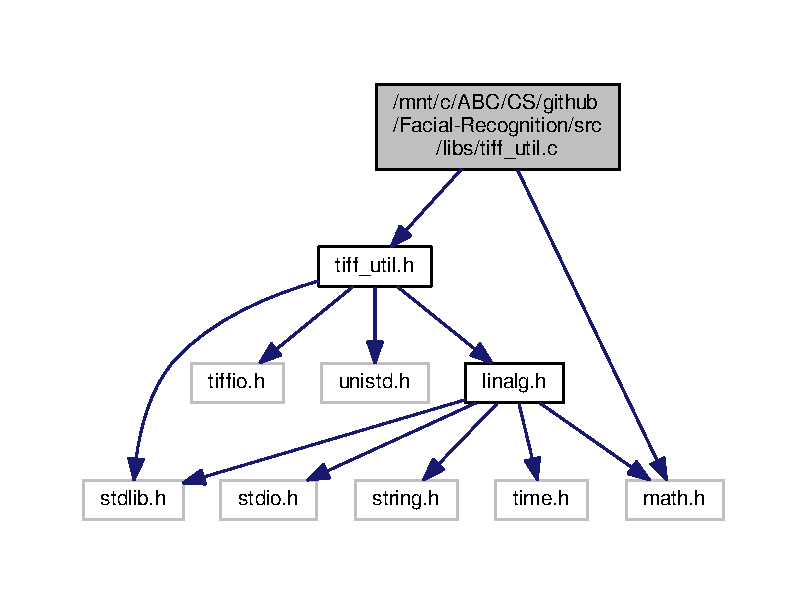
\includegraphics[width=350pt]{tiff__util_8c__incl}
\end{center}
\end{figure}
\subsection*{Functions}
\begin{DoxyCompactItemize}
\item 
\hyperlink{linalg_8h_a07a01529159cc35e78c1f7731ac7bda6}{vector} $\ast$ \hyperlink{tiff__util_8c_a62e9f072f6cc2973ba744946e6a4c5c3}{tiff\-\_\-to\-\_\-vec} (char $\ast$filename)
\begin{DoxyCompactList}\small\item\em Converts tiff to vector this function will take a T\-I\-F\-F filename and return a vector$\ast$ with every element corresponding to pixel. \end{DoxyCompactList}\item 
T\-I\-F\-F $\ast$ \hyperlink{tiff__util_8c_aa0f92f2f91378e3700ee3eb5802444b5}{vec\-\_\-to\-\_\-tiff} (char $\ast$filename, \hyperlink{linalg_8h_a07a01529159cc35e78c1f7731ac7bda6}{vector} $\ast$vec)
\begin{DoxyCompactList}\small\item\em Converts vector to tiff this function will take a vector and return a T\-I\-F\-F$\ast$ with every element corresponding to pixel. \end{DoxyCompactList}\end{DoxyCompactItemize}


\subsection{Detailed Description}
File containing common libtiff wrapper functions. Minhyuk Park \begin{DoxyDate}{Date}
9 Nov 2017 
\end{DoxyDate}


\subsection{Function Documentation}
\hypertarget{tiff__util_8c_a62e9f072f6cc2973ba744946e6a4c5c3}{\index{tiff\-\_\-util.\-c@{tiff\-\_\-util.\-c}!tiff\-\_\-to\-\_\-vec@{tiff\-\_\-to\-\_\-vec}}
\index{tiff\-\_\-to\-\_\-vec@{tiff\-\_\-to\-\_\-vec}!tiff_util.c@{tiff\-\_\-util.\-c}}
\subsubsection[{tiff\-\_\-to\-\_\-vec}]{\setlength{\rightskip}{0pt plus 5cm}{\bf vector}$\ast$ tiff\-\_\-to\-\_\-vec (
\begin{DoxyParamCaption}
\item[{char $\ast$}]{filename}
\end{DoxyParamCaption}
)}}\label{tiff__util_8c_a62e9f072f6cc2973ba744946e6a4c5c3}


Converts tiff to vector this function will take a T\-I\-F\-F filename and return a vector$\ast$ with every element corresponding to pixel. 

\begin{DoxyReturn}{Returns}
vector$\ast$ newly malloced representing the image 
\end{DoxyReturn}

\begin{DoxyParams}{Parameters}
{\em filename} & char$\ast$ the input filename \\
\hline
\end{DoxyParams}


References \-\_\-vector\-::padding, V\-E\-C, and vector\-\_\-create().


\begin{DoxyCode}
11                                     \{
12     TIFF* image = TIFFOpen(filename, \textcolor{stringliteral}{"r"});
13     uint32 width;
14     uint32 height;
15     TIFFGetField(image, TIFFTAG\_IMAGEWIDTH, &width);
16     TIFFGetField(image, TIFFTAG\_IMAGELENGTH, &height);
17 
18     uint32 num\_pixels = width * height;
19     uint32 * raster=(uint32*) \_TIFFmalloc(num\_pixels * \textcolor{keyword}{sizeof}(uint32));
20     \hyperlink{struct__vector}{vector}* retvec = \hyperlink{linalg_8c_a7040be230e99648e77b0932600bf55ef}{vector\_create}(num\_pixels);
21 
22     TIFFReadRGBAImage(image, width, height, raster, 0);
23 
24     \textcolor{keywordflow}{for}(\textcolor{keywordtype}{size\_t} i = 0; i < num\_pixels; i ++) \{
25         \hyperlink{linalg_8h_a03e904294c904b01194a25323fc2f6ec}{VEC}(retvec, i) = *(raster + i);
26     \}
27     \_TIFFfree(raster);
28 
29     retvec->\hyperlink{struct__vector_a4165a40cc39bfd874677299c943b290f}{padding} = width;
30     TIFFClose(image);
31     \textcolor{keywordflow}{return} retvec;
32 \}
\end{DoxyCode}
\hypertarget{tiff__util_8c_aa0f92f2f91378e3700ee3eb5802444b5}{\index{tiff\-\_\-util.\-c@{tiff\-\_\-util.\-c}!vec\-\_\-to\-\_\-tiff@{vec\-\_\-to\-\_\-tiff}}
\index{vec\-\_\-to\-\_\-tiff@{vec\-\_\-to\-\_\-tiff}!tiff_util.c@{tiff\-\_\-util.\-c}}
\subsubsection[{vec\-\_\-to\-\_\-tiff}]{\setlength{\rightskip}{0pt plus 5cm}T\-I\-F\-F$\ast$ vec\-\_\-to\-\_\-tiff (
\begin{DoxyParamCaption}
\item[{char $\ast$}]{filename, }
\item[{{\bf vector} $\ast$}]{vec}
\end{DoxyParamCaption}
)}}\label{tiff__util_8c_aa0f92f2f91378e3700ee3eb5802444b5}


Converts vector to tiff this function will take a vector and return a T\-I\-F\-F$\ast$ with every element corresponding to pixel. 

\begin{DoxyReturn}{Returns}
T\-I\-F\-F$\ast$ opened tiff file stream with necessary data written to from the vector 
\end{DoxyReturn}

\begin{DoxyParams}{Parameters}
{\em filename} & char$\ast$ the output filename \\
\hline
{\em vec} & vector$\ast$ vector representing the image \\
\hline
\end{DoxyParams}


References \-\_\-vector\-::padding, \-\_\-vector\-::size, and V\-E\-C.


\begin{DoxyCode}
35                                                \{
36     TIFF* rettiff = TIFFOpen(filename, \textcolor{stringliteral}{"w"});
37     uint32 width = vec->\hyperlink{struct__vector_a4165a40cc39bfd874677299c943b290f}{padding};
38     uint32 height = vec->\hyperlink{struct__vector_a1ed8dca78f3e589deb8dad9b53aec3fa}{size} / vec->\hyperlink{struct__vector_a4165a40cc39bfd874677299c943b290f}{padding};
39 
40     \textcolor{keywordtype}{char}* image\_char = malloc(vec->\hyperlink{struct__vector_a1ed8dca78f3e589deb8dad9b53aec3fa}{size} * 4); \textcolor{comment}{// 4 since RGBA}
41 
42     \textcolor{keywordflow}{for}(\textcolor{keywordtype}{size\_t} i = 0; i < vec->\hyperlink{struct__vector_a1ed8dca78f3e589deb8dad9b53aec3fa}{size}; i ++) \{
43         image\_char[4 * i] = (char)TIFFGetR((uint32)\hyperlink{linalg_8h_a03e904294c904b01194a25323fc2f6ec}{VEC}(vec, i));
44         image\_char[4 * i + 1] = (char)TIFFGetG((uint32)\hyperlink{linalg_8h_a03e904294c904b01194a25323fc2f6ec}{VEC}(vec, i));
45         image\_char[4 * i + 2] = (char)TIFFGetB((uint32)\hyperlink{linalg_8h_a03e904294c904b01194a25323fc2f6ec}{VEC}(vec, i));
46         image\_char[4 * i + 3] = (char)TIFFGetA((uint32)\hyperlink{linalg_8h_a03e904294c904b01194a25323fc2f6ec}{VEC}(vec, i));
47     \}
48     TIFFSetField (rettiff, TIFFTAG\_IMAGEWIDTH, width);
49     TIFFSetField(rettiff, TIFFTAG\_IMAGELENGTH, height);
50     TIFFSetField(rettiff, TIFFTAG\_SAMPLESPERPIXEL, 4);
51     TIFFSetField(rettiff, TIFFTAG\_BITSPERSAMPLE, 8);
52     TIFFSetField(rettiff, TIFFTAG\_ORIENTATION, ORIENTATION\_TOPLEFT);
53     TIFFSetField(rettiff, TIFFTAG\_PLANARCONFIG, PLANARCONFIG\_CONTIG);
54     TIFFSetField(rettiff, TIFFTAG\_PHOTOMETRIC, PHOTOMETRIC\_RGB);
55 
56     tsize\_t linebytes = 4 * width;
57     \textcolor{keywordtype}{unsigned} \textcolor{keywordtype}{char}* buf = NULL;
58 
59     \textcolor{keywordflow}{if} (TIFFScanlineSize(rettiff) == linebytes) \{
60         buf =(\textcolor{keywordtype}{unsigned} \textcolor{keywordtype}{char}*)\_TIFFmalloc(linebytes);
61     \} \textcolor{keywordflow}{else} \{
62         buf = (\textcolor{keywordtype}{unsigned} \textcolor{keywordtype}{char}*)\_TIFFmalloc(TIFFScanlineSize(rettiff));
63     \}
64 
65     TIFFSetField(rettiff, TIFFTAG\_ROWSPERSTRIP, TIFFDefaultStripSize(rettiff, width * 4));
66 
67     \textcolor{keywordflow}{for} (uint32 i = 0; i < height; i++)
68     \{
69         memcpy(buf, &image\_char[(height - i - 1) * linebytes], linebytes);
70         \textcolor{keywordflow}{if} (TIFFWriteScanline(rettiff, buf, i, 0) < 0) \{
71             \textcolor{keywordflow}{break};
72         \}
73     \}
74     \_TIFFfree(buf);
75     free(image\_char);
76     \textcolor{keywordflow}{return} rettiff;
77 \}\end{DoxyCode}

\hypertarget{tiff__util_8h}{\section{/mnt/c/\-A\-B\-C/\-C\-S/github/\-Facial-\/\-Recognition/src/libs/tiff\-\_\-util.h File Reference}
\label{tiff__util_8h}\index{/mnt/c/\-A\-B\-C/\-C\-S/github/\-Facial-\/\-Recognition/src/libs/tiff\-\_\-util.\-h@{/mnt/c/\-A\-B\-C/\-C\-S/github/\-Facial-\/\-Recognition/src/libs/tiff\-\_\-util.\-h}}
}


File containing common libtiff wrapper functions.  


{\ttfamily \#include $<$stdlib.\-h$>$}\\*
{\ttfamily \#include $<$tiffio.\-h$>$}\\*
{\ttfamily \#include $<$unistd.\-h$>$}\\*
{\ttfamily \#include \char`\"{}linalg.\-h\char`\"{}}\\*
Include dependency graph for tiff\-\_\-util.\-h\-:
\nopagebreak
\begin{figure}[H]
\begin{center}
\leavevmode
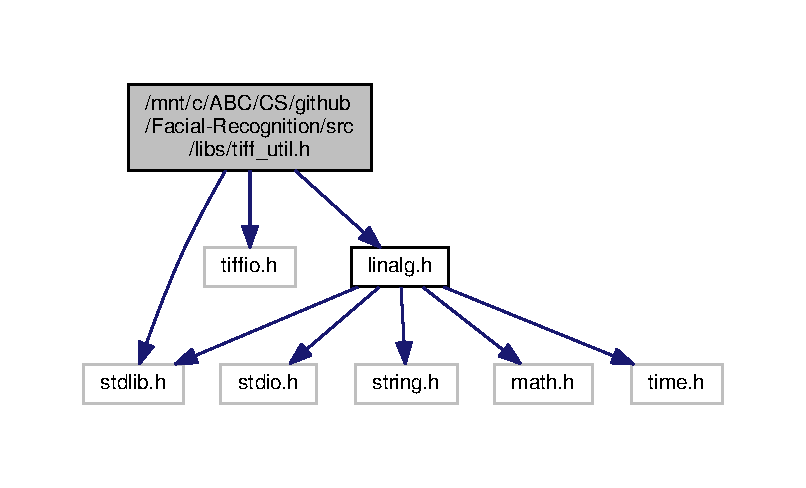
\includegraphics[width=350pt]{tiff__util_8h__incl}
\end{center}
\end{figure}
This graph shows which files directly or indirectly include this file\-:
\nopagebreak
\begin{figure}[H]
\begin{center}
\leavevmode
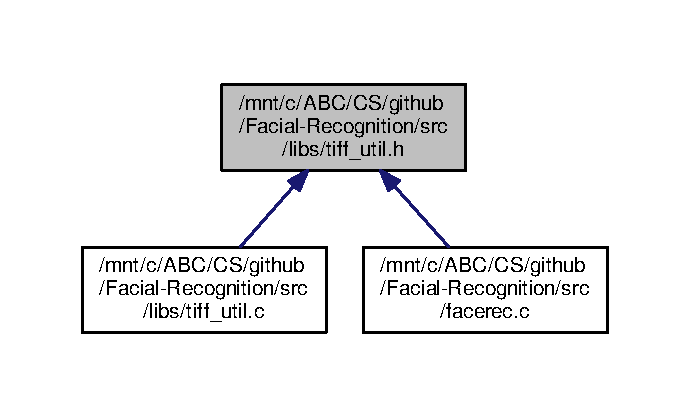
\includegraphics[width=350pt]{tiff__util_8h__dep__incl}
\end{center}
\end{figure}
\subsection*{Functions}
\begin{DoxyCompactItemize}
\item 
\hyperlink{linalg_8h_a07a01529159cc35e78c1f7731ac7bda6}{vector} $\ast$ \hyperlink{tiff__util_8h_a62e9f072f6cc2973ba744946e6a4c5c3}{tiff\-\_\-to\-\_\-vec} (char $\ast$filename)
\begin{DoxyCompactList}\small\item\em Converts tiff to vector this function will take a T\-I\-F\-F filename and return a vector$\ast$ with every element corresponding to pixel. \end{DoxyCompactList}\item 
T\-I\-F\-F $\ast$ \hyperlink{tiff__util_8h_a7ee652a16a67e21b91157392a3565ae8}{vec\-\_\-to\-\_\-tiff} (char $\ast$filename, \hyperlink{linalg_8h_a07a01529159cc35e78c1f7731ac7bda6}{vector} $\ast$vec, size\-\_\-t width, size\-\_\-t height)
\begin{DoxyCompactList}\small\item\em Converts vector to tiff this function will take a vector and return a T\-I\-F\-F$\ast$ with every element corresponding to pixel. \end{DoxyCompactList}\item 
F\-I\-L\-E $\ast$ \hyperlink{tiff__util_8h_a20075269ff8a00284dd35725029d4428}{get\-\_\-all\-\_\-tiff} (char $\ast$path, int $\ast$num\-\_\-files)
\begin{DoxyCompactList}\small\item\em Recursively earches the path for all files of .tiff type the search relies on being able to run the commands find and ls. \end{DoxyCompactList}\item 
\hyperlink{linalg_8h_a07a01529159cc35e78c1f7731ac7bda6}{vector} $\ast$ \hyperlink{tiff__util_8h_a8f8b0a0f74bb3416dd0214aa0a68130e}{tiff\-\_\-stream\-\_\-to\-\_\-vec} (F\-I\-L\-E $\ast$stream)
\begin{DoxyCompactList}\small\item\em Converts F\-I\-L\-E$\ast$ tiff stream into a vector the images are appended row-\/wise. \end{DoxyCompactList}\end{DoxyCompactItemize}


\subsection{Detailed Description}
File containing common libtiff wrapper functions. Minhyuk Park \begin{DoxyDate}{Date}
9 Nov 2017 
\end{DoxyDate}


\subsection{Function Documentation}
\hypertarget{tiff__util_8h_a20075269ff8a00284dd35725029d4428}{\index{tiff\-\_\-util.\-h@{tiff\-\_\-util.\-h}!get\-\_\-all\-\_\-tiff@{get\-\_\-all\-\_\-tiff}}
\index{get\-\_\-all\-\_\-tiff@{get\-\_\-all\-\_\-tiff}!tiff_util.h@{tiff\-\_\-util.\-h}}
\subsubsection[{get\-\_\-all\-\_\-tiff}]{\setlength{\rightskip}{0pt plus 5cm}F\-I\-L\-E$\ast$ get\-\_\-all\-\_\-tiff (
\begin{DoxyParamCaption}
\item[{char $\ast$}]{path, }
\item[{int $\ast$}]{num\-\_\-files}
\end{DoxyParamCaption}
)}}\label{tiff__util_8h_a20075269ff8a00284dd35725029d4428}


Recursively earches the path for all files of .tiff type the search relies on being able to run the commands find and ls. 

\begin{DoxyReturn}{Returns}
F\-I\-L\-E$\ast$ the stream containing all the files separated by new line characters 
\end{DoxyReturn}

\begin{DoxyParams}{Parameters}
{\em path} & char$\ast$ the path containing the files \\
\hline
{\em num\-\_\-files} & int$\ast$ outputs the number of files read \\
\hline
\end{DoxyParams}

\begin{DoxyCode}
77                                                \{
78     \textcolor{keywordtype}{char}* command = malloc(strlen(path) + 100);
79     sprintf(command, \textcolor{stringliteral}{"%s%s%s"}, \textcolor{stringliteral}{"find "}, path, \textcolor{stringliteral}{"*.tiff -type f -exec ls \{\} \(\backslash\)\(\backslash\);"});
80      
81     
82     printf(\textcolor{stringliteral}{"%s\(\backslash\)n"}, command);
83     FILE* retval = popen(command, \textcolor{stringliteral}{"r"});
84 
85     sprintf(command, \textcolor{stringliteral}{"%s%s%s"}, \textcolor{stringliteral}{"find "}, path, \textcolor{stringliteral}{"*.tiff -type f -exec ls \{\} \(\backslash\)\(\backslash\); | wc -l"});
86     
87     printf(\textcolor{stringliteral}{"%s\(\backslash\)n"}, command);
88     FILE* num\_files\_fp = popen(command, \textcolor{stringliteral}{"r"});
89     \textcolor{keywordflow}{if}(fgets(command, \textcolor{keyword}{sizeof}(command), num\_files\_fp) != NULL) \{
90         *num\_files = atoi(command);
91     \}
92     pclose(num\_files\_fp);
93     free(command);
94     \textcolor{keywordflow}{return} retval;
95 \}
\end{DoxyCode}
\hypertarget{tiff__util_8h_a8f8b0a0f74bb3416dd0214aa0a68130e}{\index{tiff\-\_\-util.\-h@{tiff\-\_\-util.\-h}!tiff\-\_\-stream\-\_\-to\-\_\-vec@{tiff\-\_\-stream\-\_\-to\-\_\-vec}}
\index{tiff\-\_\-stream\-\_\-to\-\_\-vec@{tiff\-\_\-stream\-\_\-to\-\_\-vec}!tiff_util.h@{tiff\-\_\-util.\-h}}
\subsubsection[{tiff\-\_\-stream\-\_\-to\-\_\-vec}]{\setlength{\rightskip}{0pt plus 5cm}{\bf vector}$\ast$ tiff\-\_\-stream\-\_\-to\-\_\-vec (
\begin{DoxyParamCaption}
\item[{F\-I\-L\-E $\ast$}]{stream}
\end{DoxyParamCaption}
)}}\label{tiff__util_8h_a8f8b0a0f74bb3416dd0214aa0a68130e}


Converts F\-I\-L\-E$\ast$ tiff stream into a vector the images are appended row-\/wise. 

\begin{DoxyReturn}{Returns}
vector$\ast$ newly malloced vector$\ast$ containing all the images from the stream 
\end{DoxyReturn}

\begin{DoxyParams}{Parameters}
{\em stream} & F\-I\-L\-E$\ast$ returned from \hyperlink{tiff__util_8h_a20075269ff8a00284dd35725029d4428}{get\-\_\-all\-\_\-tiff()} \\
\hline
\end{DoxyParams}


References tiff\-\_\-to\-\_\-vec(), and vec\-\_\-append().


\begin{DoxyCode}
98                                          \{
99     \textcolor{keywordtype}{char}* image\_filename;
100     \textcolor{keywordtype}{char} buffer[4096];
101 
102     \hyperlink{struct__vector}{vector}* cumulative\_image = NULL;
103     \textcolor{keywordflow}{while}(fgets(buffer, \textcolor{keyword}{sizeof}(buffer), stream) != NULL) \{
104         image\_filename = malloc(100);
105         strcpy(image\_filename, buffer);
106         image\_filename[strlen(image\_filename) - 1] = \textcolor{charliteral}{'\(\backslash\)0'};
107         \textcolor{keywordflow}{if}(cumulative\_image == NULL) \{
108             cumulative\_image = \hyperlink{tiff__util_8c_a62e9f072f6cc2973ba744946e6a4c5c3}{tiff\_to\_vec}(image\_filename);
109         \} \textcolor{keywordflow}{else} \{
110             \hyperlink{linalg_8c_adbfad21fe7e851455d625173e67b8504}{vec\_append}(&cumulative\_image, \hyperlink{tiff__util_8c_a62e9f072f6cc2973ba744946e6a4c5c3}{tiff\_to\_vec}(image\_filename));
111         \}
112         free(image\_filename);
113     \}
114     \textcolor{keywordflow}{return} cumulative\_image;
115 \}\end{DoxyCode}
\hypertarget{tiff__util_8h_a62e9f072f6cc2973ba744946e6a4c5c3}{\index{tiff\-\_\-util.\-h@{tiff\-\_\-util.\-h}!tiff\-\_\-to\-\_\-vec@{tiff\-\_\-to\-\_\-vec}}
\index{tiff\-\_\-to\-\_\-vec@{tiff\-\_\-to\-\_\-vec}!tiff_util.h@{tiff\-\_\-util.\-h}}
\subsubsection[{tiff\-\_\-to\-\_\-vec}]{\setlength{\rightskip}{0pt plus 5cm}{\bf vector}$\ast$ tiff\-\_\-to\-\_\-vec (
\begin{DoxyParamCaption}
\item[{char $\ast$}]{filename}
\end{DoxyParamCaption}
)}}\label{tiff__util_8h_a62e9f072f6cc2973ba744946e6a4c5c3}


Converts tiff to vector this function will take a T\-I\-F\-F filename and return a vector$\ast$ with every element corresponding to pixel. 

\begin{DoxyReturn}{Returns}
vector$\ast$ newly malloced representing the image 
\end{DoxyReturn}

\begin{DoxyParams}{Parameters}
{\em filename} & char$\ast$ the input filename \\
\hline
\end{DoxyParams}


References \-\_\-vector\-::padding, V\-E\-C, and vector\-\_\-create().



Referenced by tiff\-\_\-stream\-\_\-to\-\_\-vec().


\begin{DoxyCode}
11                                     \{
12     TIFF* image = TIFFOpen(filename, \textcolor{stringliteral}{"r"});
13     uint32 width;
14     uint32 height;
15     TIFFGetField(image, TIFFTAG\_IMAGEWIDTH, &width);
16     TIFFGetField(image, TIFFTAG\_IMAGELENGTH, &height);
17 
18     uint32 num\_pixels = width * height;
19     uint32 * raster=(uint32*) \_TIFFmalloc(num\_pixels * \textcolor{keyword}{sizeof}(uint32));
20     \hyperlink{struct__vector}{vector}* retvec = \hyperlink{linalg_8c_a7040be230e99648e77b0932600bf55ef}{vector\_create}(num\_pixels);
21 
22     TIFFReadRGBAImage(image, width, height, raster, 0);
23 
24     \textcolor{keywordflow}{for}(\textcolor{keywordtype}{size\_t} i = 0; i < num\_pixels; i ++) \{
25         \hyperlink{linalg_8h_a03e904294c904b01194a25323fc2f6ec}{VEC}(retvec, i) = *(raster + i);
26     \}
27     \_TIFFfree(raster);
28 
29     retvec->\hyperlink{struct__vector_a4165a40cc39bfd874677299c943b290f}{padding} = width;
30     TIFFClose(image);
31     \textcolor{keywordflow}{return} retvec;
32 \}
\end{DoxyCode}
\hypertarget{tiff__util_8h_a7ee652a16a67e21b91157392a3565ae8}{\index{tiff\-\_\-util.\-h@{tiff\-\_\-util.\-h}!vec\-\_\-to\-\_\-tiff@{vec\-\_\-to\-\_\-tiff}}
\index{vec\-\_\-to\-\_\-tiff@{vec\-\_\-to\-\_\-tiff}!tiff_util.h@{tiff\-\_\-util.\-h}}
\subsubsection[{vec\-\_\-to\-\_\-tiff}]{\setlength{\rightskip}{0pt plus 5cm}T\-I\-F\-F$\ast$ vec\-\_\-to\-\_\-tiff (
\begin{DoxyParamCaption}
\item[{char $\ast$}]{filename, }
\item[{{\bf vector} $\ast$}]{vec, }
\item[{size\-\_\-t}]{width, }
\item[{size\-\_\-t}]{height}
\end{DoxyParamCaption}
)}}\label{tiff__util_8h_a7ee652a16a67e21b91157392a3565ae8}


Converts vector to tiff this function will take a vector and return a T\-I\-F\-F$\ast$ with every element corresponding to pixel. 

\begin{DoxyReturn}{Returns}
T\-I\-F\-F$\ast$ opened tiff file stream with necessary data written to from the vector 
\end{DoxyReturn}

\begin{DoxyParams}{Parameters}
{\em filename} & char$\ast$ the output filename \\
\hline
{\em vec} & vector$\ast$ vector representing the image \\
\hline
{\em width} & size\-\_\-t width of the image \\
\hline
{\em height} & size\-\_\-t height of the image \\
\hline
\end{DoxyParams}


References \-\_\-vector\-::size, and V\-E\-C.


\begin{DoxyCode}
35                                                                             \{
36     TIFF* rettiff = TIFFOpen(filename, \textcolor{stringliteral}{"w"});
37 
38     \textcolor{keywordtype}{char}* image\_char = malloc(vec->\hyperlink{struct__vector_a1ed8dca78f3e589deb8dad9b53aec3fa}{size} * 4); \textcolor{comment}{// 4 since RGBA}
39 
40     \textcolor{keywordflow}{for}(\textcolor{keywordtype}{size\_t} i = 0; i < vec->\hyperlink{struct__vector_a1ed8dca78f3e589deb8dad9b53aec3fa}{size}; i ++) \{
41         image\_char[4 * i] = (char)TIFFGetR((uint32)\hyperlink{linalg_8h_a03e904294c904b01194a25323fc2f6ec}{VEC}(vec, i));
42         image\_char[4 * i + 1] = (char)TIFFGetG((uint32)\hyperlink{linalg_8h_a03e904294c904b01194a25323fc2f6ec}{VEC}(vec, i));
43         image\_char[4 * i + 2] = (char)TIFFGetB((uint32)\hyperlink{linalg_8h_a03e904294c904b01194a25323fc2f6ec}{VEC}(vec, i));
44         image\_char[4 * i + 3] = (char)TIFFGetA((uint32)\hyperlink{linalg_8h_a03e904294c904b01194a25323fc2f6ec}{VEC}(vec, i));
45     \}
46     TIFFSetField (rettiff, TIFFTAG\_IMAGEWIDTH, width);
47     TIFFSetField(rettiff, TIFFTAG\_IMAGELENGTH, height);
48     TIFFSetField(rettiff, TIFFTAG\_SAMPLESPERPIXEL, 4);
49     TIFFSetField(rettiff, TIFFTAG\_BITSPERSAMPLE, 8);
50     TIFFSetField(rettiff, TIFFTAG\_ORIENTATION, ORIENTATION\_TOPLEFT);
51     TIFFSetField(rettiff, TIFFTAG\_PLANARCONFIG, PLANARCONFIG\_CONTIG);
52     TIFFSetField(rettiff, TIFFTAG\_PHOTOMETRIC, PHOTOMETRIC\_RGB);
53 
54     tsize\_t linebytes = 4 * width;
55     \textcolor{keywordtype}{unsigned} \textcolor{keywordtype}{char}* buf = NULL;
56 
57     \textcolor{keywordflow}{if} (TIFFScanlineSize(rettiff) == linebytes) \{
58         buf =(\textcolor{keywordtype}{unsigned} \textcolor{keywordtype}{char}*)\_TIFFmalloc(linebytes);
59     \} \textcolor{keywordflow}{else} \{
60         buf = (\textcolor{keywordtype}{unsigned} \textcolor{keywordtype}{char}*)\_TIFFmalloc(TIFFScanlineSize(rettiff));
61     \}
62 
63     TIFFSetField(rettiff, TIFFTAG\_ROWSPERSTRIP, TIFFDefaultStripSize(rettiff, width * 4));
64 
65     \textcolor{keywordflow}{for} (uint32 i = 0; i < height; i++) \{
66         memcpy(buf, &image\_char[(height - i - 1) * linebytes], linebytes);
67         \textcolor{keywordflow}{if} (TIFFWriteScanline(rettiff, buf, i, 0) < 0) \{
68             \textcolor{keywordflow}{break};
69         \}
70     \}
71     \_TIFFfree(buf);
72     free(image\_char);
73     \textcolor{keywordflow}{return} rettiff;
74 \}
\end{DoxyCode}

%--- End generated contents ---

% Index
\newpage
\phantomsection
\addcontentsline{toc}{chapter}{Index}
\printindex

\end{document}
